\documentclass[12pt,a4paper]{article}
\usepackage[spanish,es-tabla]{babel}
\usepackage[utf8]{inputenc}
\usepackage[T1]{fontenc}
\usepackage{graphicx}
\graphicspath{{Imagenes/}}
\usepackage[colorlinks=true, urlcolor=black, linkcolor=black]{hyperref}
\usepackage{amsmath,amssymb,mathtools}
\usepackage{siunitx}
\usepackage{hyperref}
\usepackage{csquotes}
\usepackage{titling}
\usepackage[font=footnotesize]{caption}
\usepackage{float}
\usepackage[spanish]{babel}
\usepackage[utf8]{inputenc}
\usepackage{graphicx}
\usepackage{geometry}
\geometry{margin=2.5cm}
\usepackage{booktabs}
\usepackage{tabularx}
\usepackage{sectsty} % <-- AÑADIR ESTE PAQUETE

\sectionfont{\LARGE}
\subsectionfont{\Large}
\subsubsectionfont{\large}
\numberwithin{figure}{section}
\numberwithin{equation}{section}
\begin{document}

% === Carátula ===
\begin{titlepage}
\begin{center}

% --- Escudo ---

\includegraphics[width=6cm]{Escudo.png}\\[1.5cm] % 
\textit{Facultad de Ciencias Exactas, Físicas y Naturales\\
Universidad Nacional de Córdoba}\\
[2.0cm]
% --- Subtítulo ---
{\LARGE \textbf{Amplificadores  Integrados Lineales}}\\[2.0cm]
{\large Cátedra de Síntesis de Redes Activas 
2026}\\[2.0cm]
\hrule height 1pt
\vspace{0.5cm}
\hrule height 1pt
\vspace{2cm}

% --- Autor ---
\textbf{Autor:} Ing. Oscar Puigdellibo\\[1.0cm]
\textbf{Revisado y Actualizado por:}  
Ing. Pablo A. Ferreyra \\[0.5cm] 
Profesor Titular de la Cátedra de Síntesis de Redes Activas  
Facultad de Ciencias Exactas, Físicas y Naturales  
Universidad Nacional de Córdoba\\[1cm]

\vfill


\end{center}
\end{titlepage}
\clearpage


%\maketitle
\tableofcontents
\clearpage

\begin{thebibliography}{99}
\setlength{\itemsep}{0.25em}
\setlength{\parskip}{0pt}
\setlength{\parsep}{0pt}
\subsection*{Textos}
\bibitem{millman}
J.~Millman and A.~Grabel,
``Microelectrónica,''
\emph{McGraw-Hill},
Nueva York, NY, USA, 1987.

\bibitem{herpy}
M.~Herpy,
``Analog Integrated Circuits,''
\emph{John Wiley \& Sons},
Nueva York, NY, USA, 1980.

\bibitem{frederiksen}
T.~M. Frederiksen,
``Intuitive IC Op Amps,''
\emph{National Semiconductor Corp.},
Santa Clara, CA, USA, 1984.

\bibitem{rashid}
M.~H. Rashid,
``Circuitos Microelectrónicos: Análisis y Diseño,''
\emph{Thomson Editores},
México, 2000.

\bibitem{tobey}
G.~E. Tobey, J.~G. Graeme, and L.~P. Huelsman,
``Operational Amplifiers: Design and Applications,''
\emph{McGraw-Hill},
Nueva York, NY, USA, 1971.
\subsection*{Notas Técnicas}
\bibitem{wong}
J.~Wong and A.~García,
``Precision Transducer Interfaces,''
\emph{Analog Devices},
Amplifiers Applications Guide, 1992.

\bibitem{kester}
W.~Kester, S.~Wurcer, and C.~Kitchin,
``High Impedance, Low Current Applications,''
\emph{Analog Devices},
Amplifiers Applications Guide, 1992.

\bibitem{burr_ab090}
``Op Amp Performance Análisis,''
\emph{Burr-Brown},
AB-090.

\bibitem{burr_ab075}
``Photodiode Monitoring with Operational Amplifiers,''
\emph{Burr Brown},
AB-075.

\bibitem{national_oa25}
``Stability Analisis of  Current Feedback Amplifiers,''
\emph{National Semiconductors},
OA25, May 1995.

\bibitem{intersil_an9420}
``Current Feedback Amplifiers-Theory and Applications,''
\emph{Intersil},
AN9420.1, April 1995.

\bibitem{national_oa07}
``Current Feedback  OP. Amp – Applications Circuits Guide,''
\emph{National Semiconductors},
OA 07, May 1988.

\bibitem{ti_opa684}
``OPA-684- Current Feedback Amplifiers- (Applications),''
\emph{Texas Instrument},
SBOS219A.

\bibitem{burr_ab091}
``Voltage –Feedback Amplifiers vs Current Feedback Amplifiers,''
\emph{Burr Brown},
AB-091.

\bibitem{burr_ab193}
``The Current Feedback Op-Amp a High Speed Building Block,''
\emph{Burr-Brown},
AB -193.
\bibitem{burr_ab183}
``New Ultra High –Speed Circuits Techniques with Analog ICs,''
\emph{Burr-Brown},
AB- 183.

\bibitem{burr_ab180}
``Ultra High Speed ICs,''
\emph{Burr Brown},
AB-180.

\bibitem{national_1996}
``National Linear Seminar-1996,''
\emph{National Semiconductors}.

\bibitem{dualibe}
C.~F. Dualibe,
``GMC,''
\emph{Edición Interna}.
\end{thebibliography}
\section*{Introducción}
Este texto tratará el análisis y diseño de circuitos con amplificadores lineales integrados. El capítulo I y II están dedicados al amplificador operacional 
clásico, modernamente identificado por los fabricantes como realimentado por 
tensión, (Voltage Feedback Amplifier), para diferenciarlo de otros tipos. \\
Únicamente se analizaran las aplicaciones de las configuraciones realimentadas, 
utilizando  en el análisis las técnicas y conclusiones de este tipo de sistemas. \\
En el  capítulo. 
I, se tratará el amplificador ideal a los efectos de familiarizase  
con técnicas operativas clásicas y definir magnitudes que serán referencias. 
Para el  estudio del capítulo II, que se centrará en el amplificador operacional 
real, con función de transferencia de un solo polo (Internamente compensado), 
donde se analizarán las desviaciones producidas por sus características reales, 
profundizando aquellas que se refieren a la respuesta en frecuencia del conjunto que son generalmente el punto crítico en la síntesis de amplificadores de 
banda ancha. En el capítulo III se estudiará otro tipo de amplificador de muy 
alta ganancia y velocidad, denominado  realimentado por corriente, (CFA) 
mientras que el IV, lo hará con los amplificadores de transconductancia, 
(O.T.A), en sus dos variantes (tecnología VFA y CFA). El capítulo V y parte del 
VI tratan temas generales respecto del modelado de la respuesta en frecuencia 
de redes activas  (Realimentadas o Directas), cuyas conclusiones serán de 
aplicación en la síntesis de amplificadores en lo que resta del texto.
\newpage
\section{Amplificador ideal realimentado por tensión (VFA)}
\subsection*{Introducción}
El modelo asumido en la Figura~\ref{fig:1.1} describe con bastante exactitud el comportamiento con pequeña señal de un A.O.\ clásico. Es importante destacar el orden de magnitud de los parámetros involucrados en el modelo asumido. Así, la impedancia de entrada de modo diferencial ($Z_{id}$) es muy elevada, siendo su componente resistiva superior al M$\Omega$ y la capacitiva apenas unos pocos picofaradios; de igual manera la impedancia de modo común ($Z_c$), cuyos valores son mayores a aquella en uno o dos órdenes de magnitud. En cambio, la impedancia de salida es muy baja (decenas de $\Omega$). El generador controlado de salida ($A(s)$) tiene dos componentes: la de modo diferencial $A_d(s)$, muy elevada (típico 100 dB), y la de modo común muy baja, definida generalmente a través de la relación de rechazo de modo común ($RRMC=A_d/A_c$).
\begin{figure}[H]
    \centering
    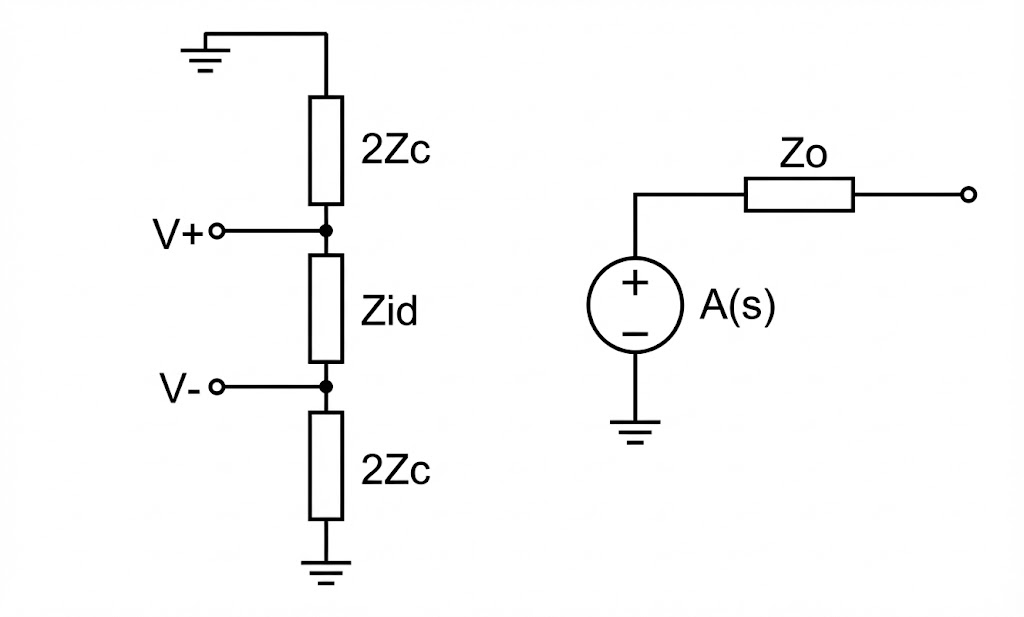
\includegraphics[width=0.5\linewidth]{Imagenes/1.1.png}
    \caption{Modelo del Amplificador  Operacional Real.}
    \label{fig:1.1}
\end{figure}
En general, interesa evaluar los efectos de primer orden que las características reales imponen sobre el comportamiento del amplificador. Si bien ciertos efectos críticos en una aplicación pueden resultar irrelevantes en otra, es posible asumir un modelo real simplificado, como se observa en la Figura~\ref{fig:1.2}a, que permita evaluar al menos los parámetros típicos; este análisis se abordará en el capítulo siguiente. Por otro lado, la Figura~\ref{fig:1.2}b presenta el modelo lineal de pequeña señal idealizado, el cual será utilizado en el desarrollo subsiguiente.
\begin{figure}[H]
    \centering
    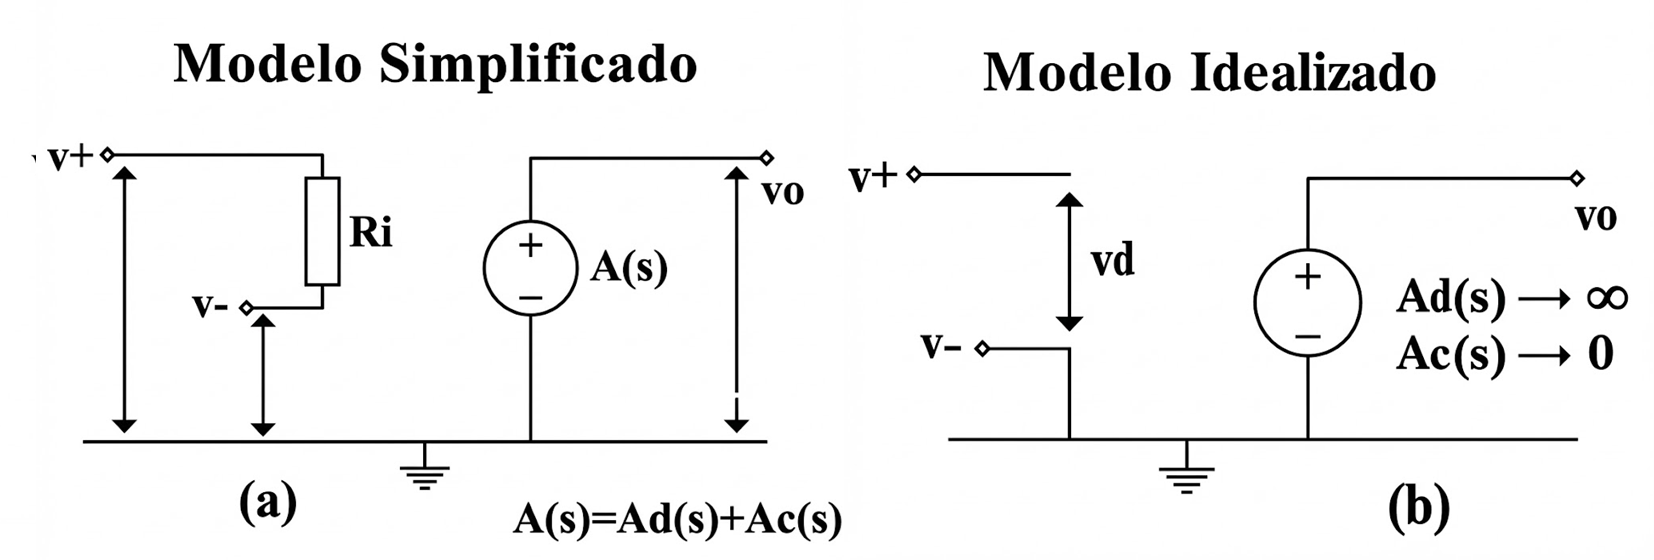
\includegraphics[width=0.85\linewidth]{Imagenes/1.2.png}
    \caption{Modelos del amplificador operacional}
    \label{fig:1.2}
\end{figure}
La figura ~\ref{fig:1.3}a muestra la estructura clásica de utilización del amplificador operacional, con la red de realimentación conectada. Esta es generalmente un cuadripolo pasivo (R-C) con un terminal común ~\ref{fig:1.3}b.
\begin{figure}[H]
    \centering
    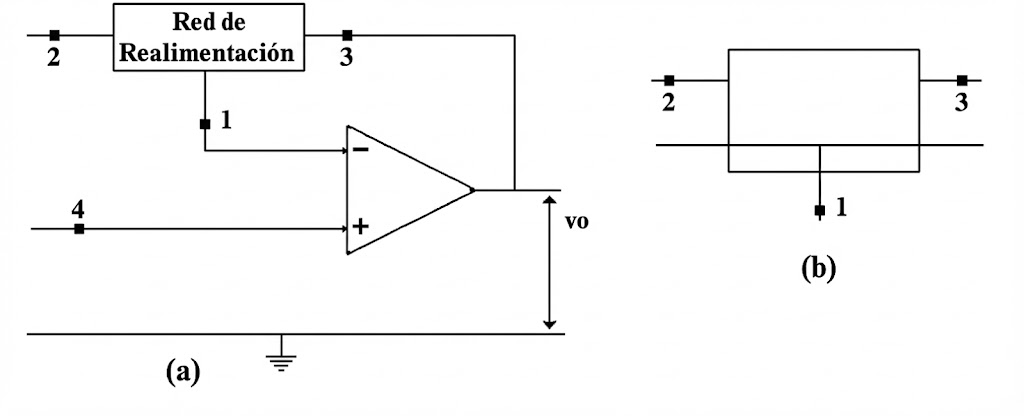
\includegraphics[width=0.85\linewidth]{Imagenes/1.3.png}
    \caption{Realimentación de un amplificador operacional}
    \label{fig:1.3}
\end{figure}
Dependiendo de si la señal excita el terminal (2), el (4) o ambos simultáneamente, se obtienen configuraciones inversoras, no inversoras o diferenciales, respectivamente. La utilización del modelo idealizado simplifica notablemente el análisis del circuito. Por ejemplo, considerar una impedancia de entrada infinita trae consigo las siguientes implicaciones:
\begin{figure}[H]
    \centering
    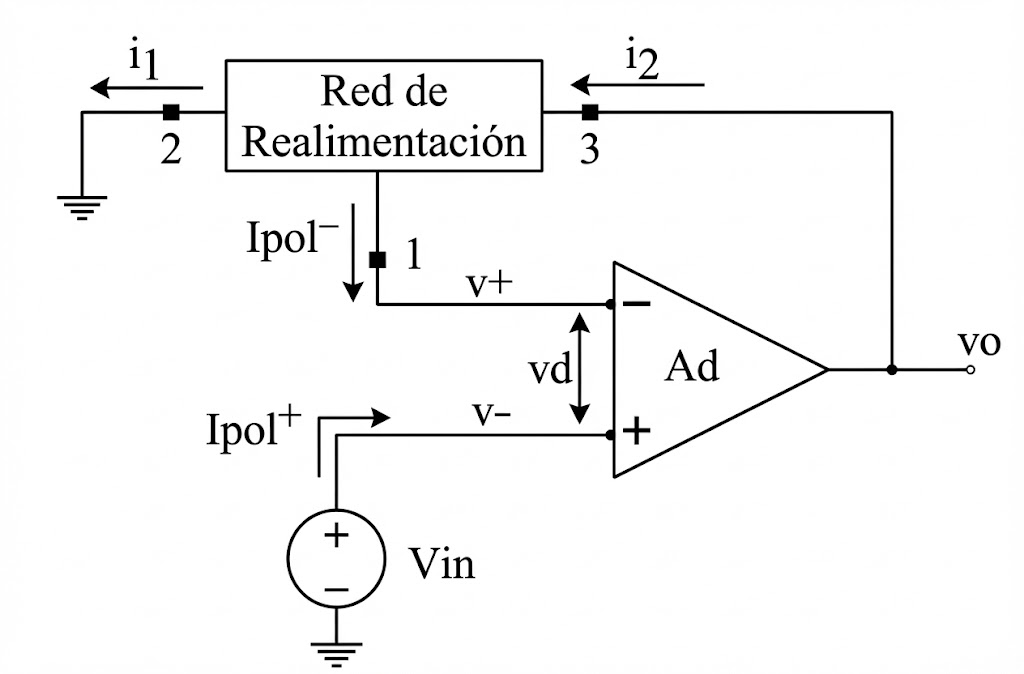
\includegraphics[width=0.5\linewidth]{Imagenes/1.4.png}
    \caption{Realimentación de un amplificador operacional}
    \label{fig:1.4}
\end{figure}
\vspace{-1.5em}
\begin{equation}
    Z_{id} \to \infty \implies I_{pol}^{-} = 0 \implies i_1 = i_2
    \label{eq:1.1}
\end{equation}

Además, si se considera una ganancia de modo diferencial infinita ($A_d \to \infty$), la única posibilidad de obtener una tensión de salida finita (según $v_o = A_d \cdot v_d$) es asegurando una tensión diferencial de entrada nula. Este hecho solo es posible retornando una fracción ($K$) de la señal de salida al terminal inversor con la fase apropiada (realimentación negativa), lo que conduce a:
\begin{equation}
    A_d \to \infty \implies v_d = (v^+ - v^-) \to 0 \implies v^+ = v^-
    \label{eq:1.2}
\end{equation}

La asunción hecha se traduce en un ``cortocircuito virtual'' a la entrada del amplificador. Si, sumadas a las conclusiones obtenidas, se consideran además la ganancia de modo común y la impedancia de salida nulas, la mayoría de las configuraciones básicas con A.O.\ se resuelven por simple inspección.
\subsection{Aplicaciones Lineales}
En la mayoría de las configuraciones, la red de realimentación es simplemente un divisor resistivo que ajusta la cantidad de realimentación introducida a la entrada inversora ($k \cdot v_o$), tal como muestra la Figura~\ref{fig:1.5} para los circuitos denominados inversor y no inversor. Para el primero de ellos, las conclusiones \eqref{eq:1.1} y \eqref{eq:1.2} llevan a:
\begin{equation}
    v^+ = v^- = 0 \quad \text{e} \quad i_2 = i_1 \implies \frac{v_o}{R_2} = -\frac{v_{in}}{R_1}
    \label{eq:1.3}
\end{equation}
\begin{figure}[H]
    \centering
    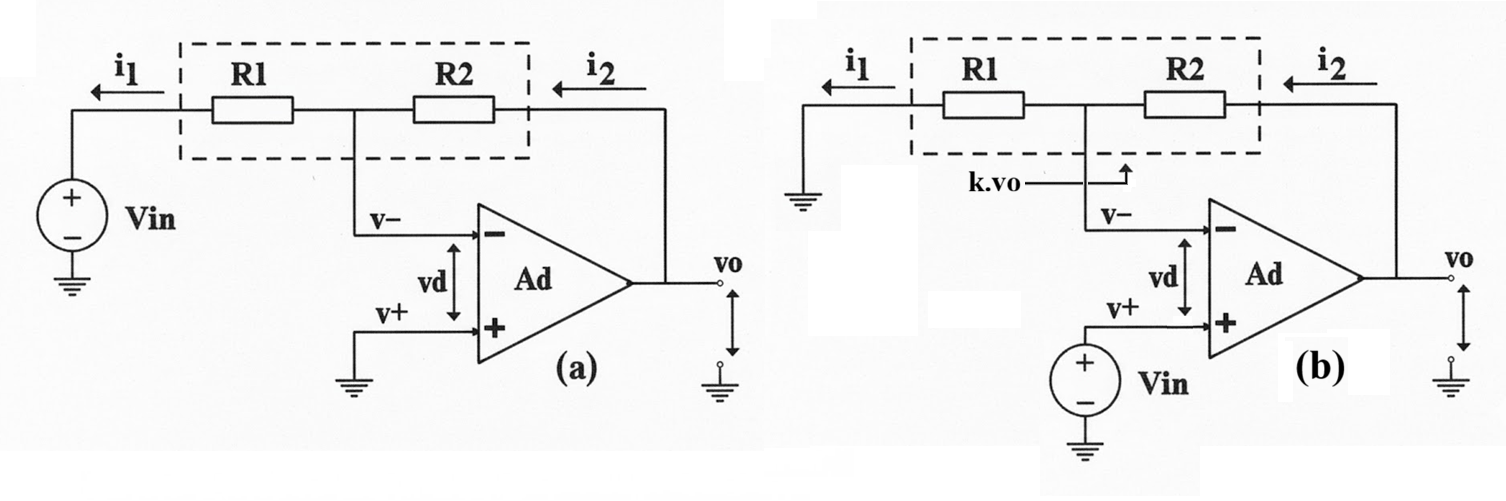
\includegraphics[width=0.95\linewidth]{Imagenes/1.5.png}
    \caption{Amplificador inversor}
    \label{fig:1.5}
\end{figure}
Luego:
\begin{equation}
    A_{vfi} = \frac{v_o}{v_{in}} = -\frac{R_2}{R_1} \qquad A_{vfi} = \text{Ganancia de tensión ideal.}
    \label{eq:1.4}
\end{equation}

Teniendo en cuenta que:
\begin{equation}
    K = \frac{R_1}{R_1 + R_2} \implies A_{vfi} = \left( 1 - \frac{1}{K} \right)
    \label{eq:1.5}
\end{equation}

De igual manera en el circuito no inversor:
\begin{equation}
    i_1 = i_2 \implies \frac{v_o - v^+}{R_2} = \frac{v^-}{R_1}
    \label{eq:1.6}
\end{equation}

\begin{equation}
    v^+ = v^- = v_{in} \implies A_{vfi} = \frac{R_1 + R_2}{R_1} = 1 + \frac{R_2}{R_1} = \frac{1}{K}
    \label{eq:1.7}
\end{equation}
La figura ~\ref{fig:1.6} muestra una configuración que esta excitada en los dos terminales en la que se demuestra que la tensión de salida es proporcional al modo diferencial de las señales de entrada.
\begin{figure}[H]
    \centering
    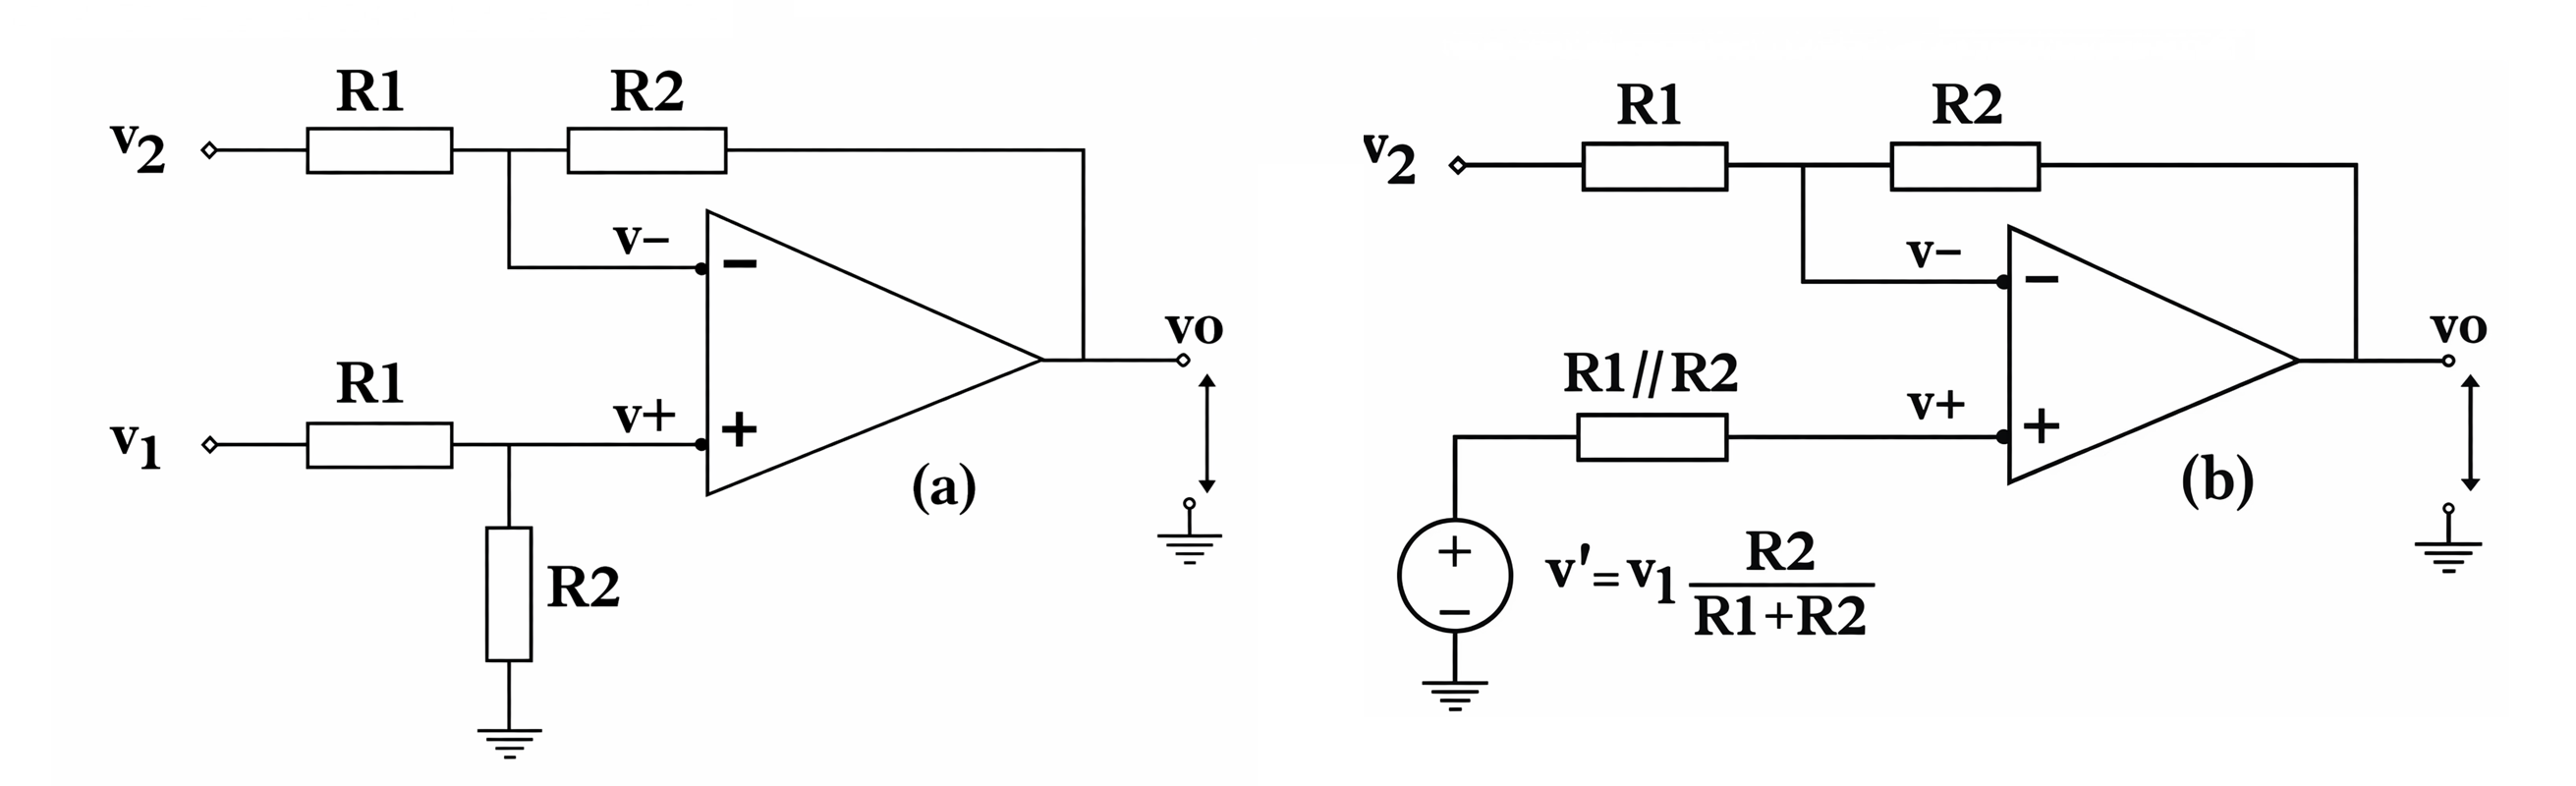
\includegraphics[width=0.95\linewidth]{Imagenes/1.6.png}
    \caption{Modo diferencial}
    \label{fig:1.6}
\end{figure}
En efecto, utilizando superposición queda una configuración inversora al pasivar $V_1$, y no inversora al hacerlo con $V_2$; luego, utilizando las conclusiones anteriores \eqref{eq:1.4} y \eqref{eq:1.7} se obtiene:

\[
v_0 = \left[ -\frac{R_2}{R_1} \cdot v_2 \right]_{V_1 = 0} + \left[ v' \cdot \left( 1 + \frac{R_2}{R_1} \right) \right]_{V_2 = 0}
\]

La que luego de operarla lleva a: 
\begin{equation}
    v_0 = (v_1 - v_2) \frac{R_2}{R_1} \implies A_{vfi} = \frac{v_0}{v_1 - v_2} = \frac{R_2}{R_1}
    \label{eq:1.8}
\end{equation}
\vspace{1em} % Espacio opcional antes del bloque
\hrule height 1.5pt % Línea gruesa superior
\vspace{2pt}
\noindent {\large \textbf{Problema.}}
\vspace{4pt}
\hrule height 1pt % Línea inferior
\vspace{1.5em}

Utilizando superposición, demuestre que la tensión de salida del diferencial de la figura es:

\[
v_o = (v_2 - v_1) + v_X
\]
\vspace{-2em}
\begin{figure}[H]
    \centering
    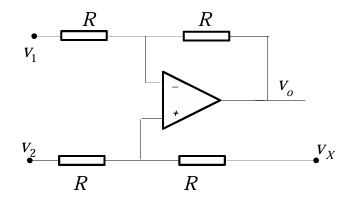
\includegraphics[width=0.5\linewidth]{Imagenes/1.E.png}
\end{figure}
\hrule height 1.5pt % Línea gruesa superior
\vspace{2pt}
Para generar funciones de filtros (pasa bajos, pasa banda, etc.), la red de realimentación está compuesta por resistores y capacitores. Aquellos circuitos que realizan funciones de primer grado (un polo o un cero real) también pueden analizarse por simple inspección. Por ejemplo, el que muestra la Figura~\ref{fig:1.7} es un filtro pasa alto inversor de grado uno.
\begin{figure}[H]
    \centering
    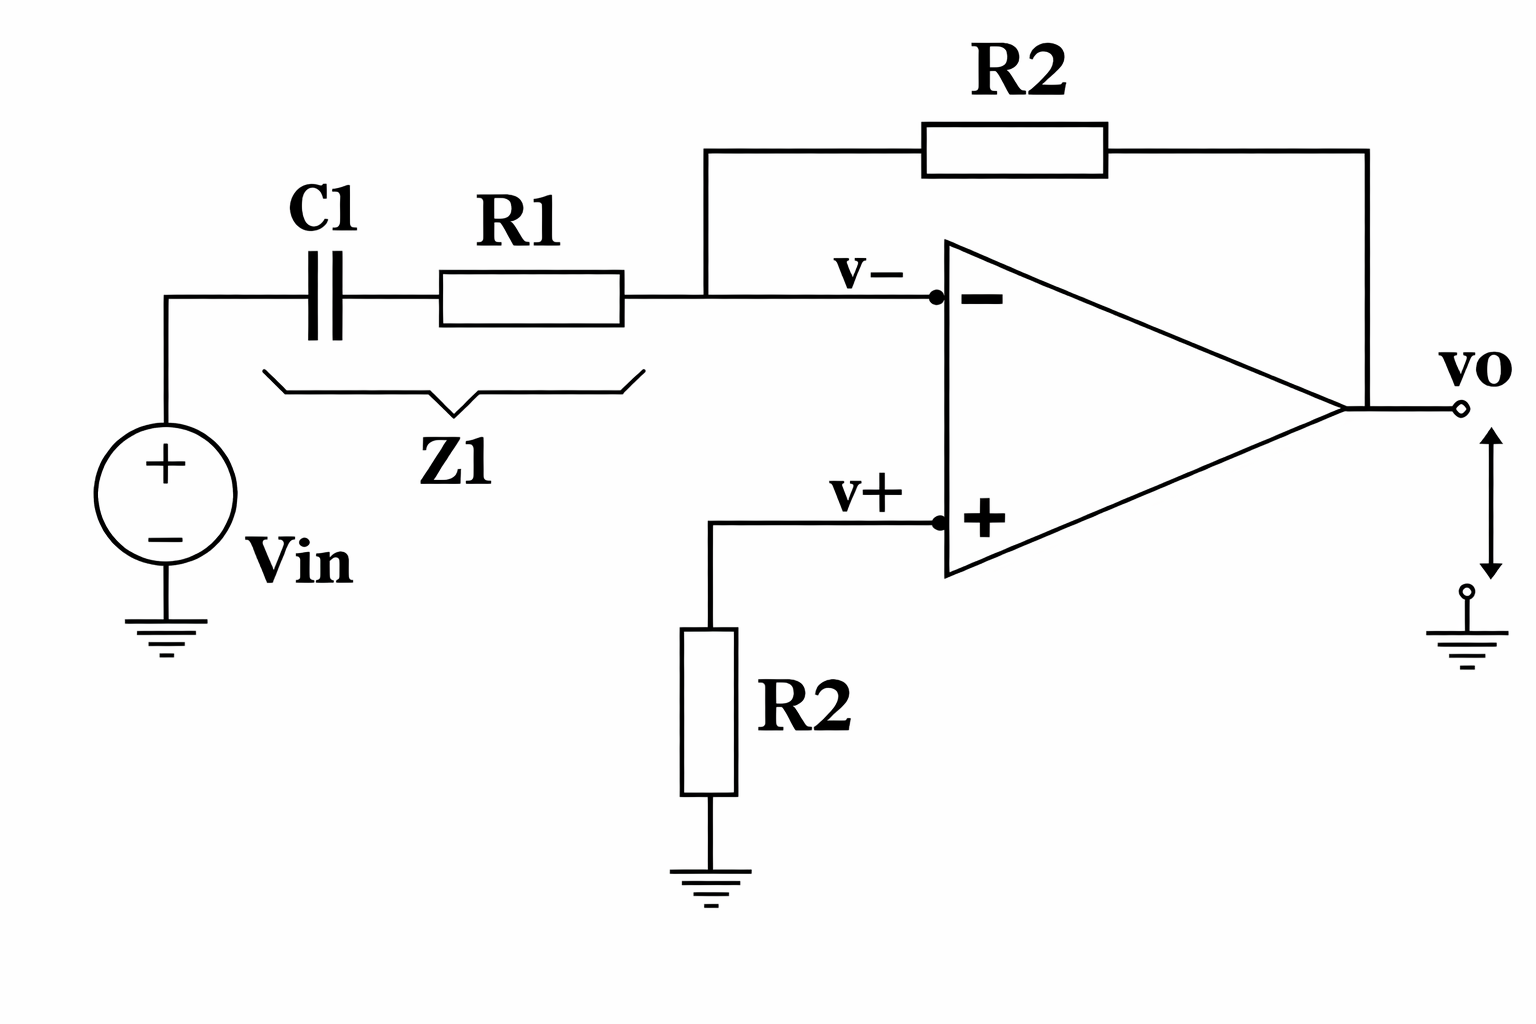
\includegraphics[width=0.5\linewidth]{Imagenes/1.7.png}
    \caption{Filtro pasa alto}
    \label{fig:1.7}
\end{figure}
Tratándose de una configuración inversora, su ganancia es:

\begin{align}
    A_{vf}(s) &= -\frac{R_2}{Z_1} = -\frac{R_2}{R_1 + \dfrac{1}{s \cdot C_1}} = -\frac{s \cdot C_1 \cdot R_2}{1 + s \cdot C_1 \cdot R_1} \notag \\
    \notag \\
    A_{vf}(s) &= -\frac{R_2}{R_1} \cdot \frac{s}{s + a} = -A_{vf}(\infty) \cdot \frac{s}{s + a} \label{eq:1.9} \\
    A_{vf}(\infty) &= \frac{R_2}{R_1} \to \text{(Asíntota de alta frecuencia)} \notag
\end{align}

Es interesante comparar la respuesta del circuito activo de la Figura~\ref{fig:1.7} con la de un filtro pasivo equivalente. El circuito pasivo en cuestión se muestra en la Figura~\ref{fig:1.8}, y su F.T.\ es la siguiente:

\begin{nointerlineskip}
\begin{minipage}{0.5\textwidth}
    \begin{align*}
        A_v(s) &= \frac{v_0}{v_{in}} = \frac{s}{s + \dfrac{1}{C_1 \cdot R_1}} = \frac{s}{s + a} \\
        A_{vf}(\infty) &= 1
    \end{align*}
\end{minipage}
\begin{minipage}{0.5\textwidth}
    \centering
    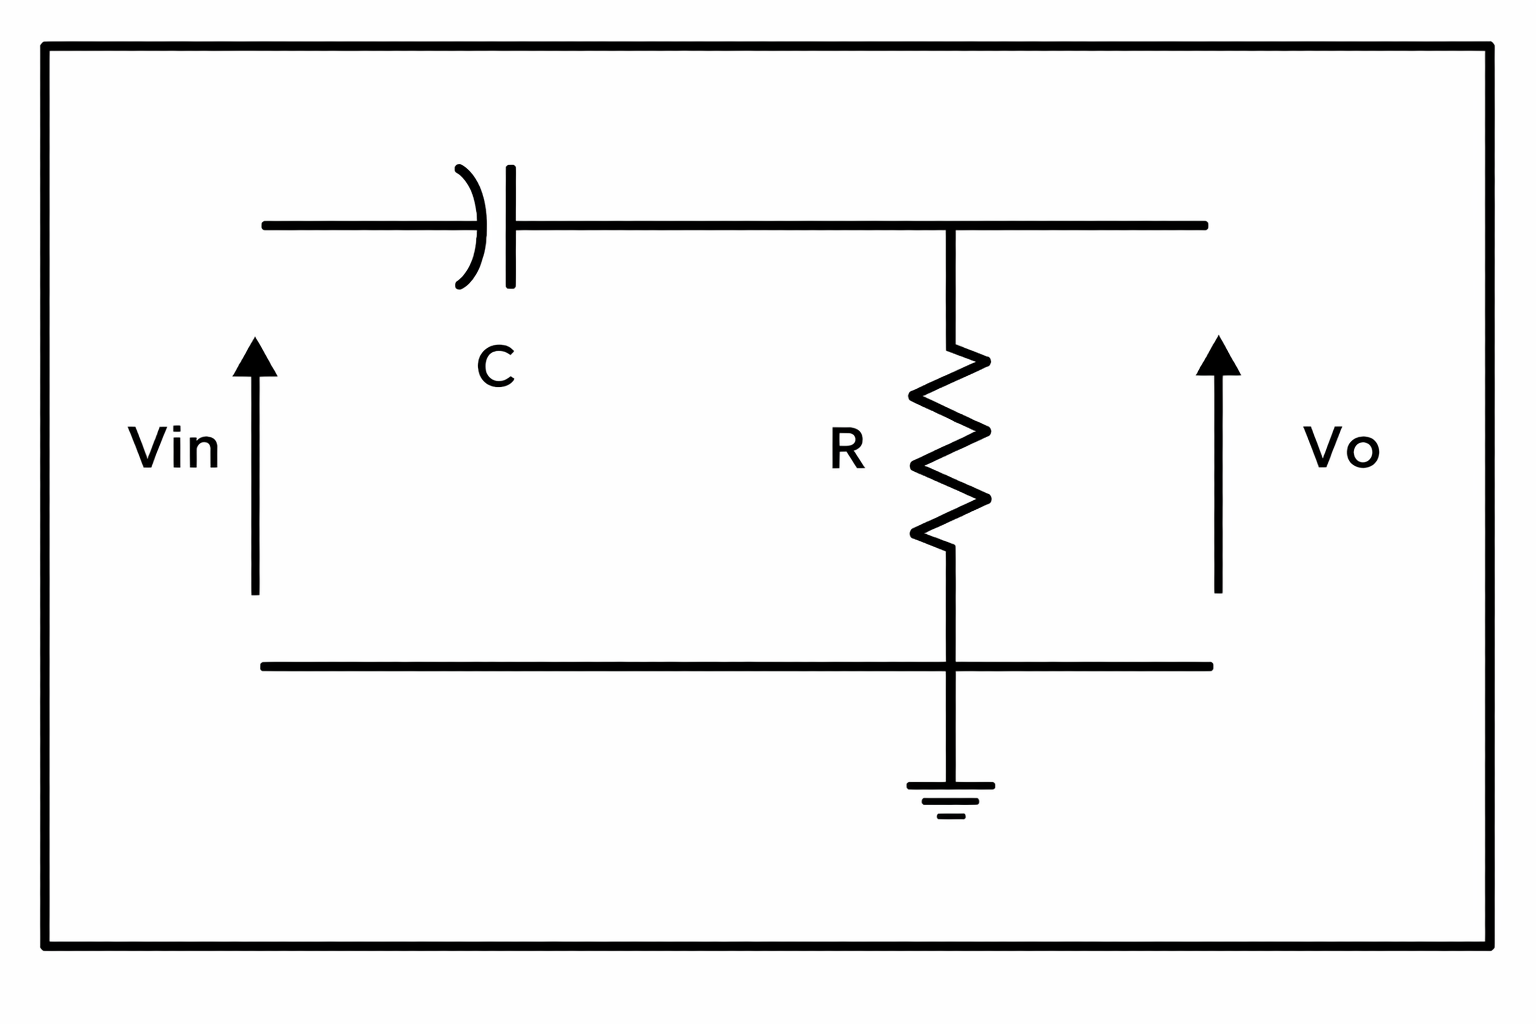
\includegraphics[width=0.7\linewidth]{Imagenes/1.8.png}
    \captionof{figure}{Filtro RC pasivo}
    \label{fig:1.8}
\end{minipage}
\end{nointerlineskip}

Comparando las funciones de transferencia anteriores, se aprecia la ganancia adicional que aporta el filtro activo en la banda de paso ($A_{vf}(\infty) = R_2/R_1 > 1$), frente a la máxima que puede otorgar su homónimo pasivo, que es la unidad. En el diagrama de la Figura~\ref{fig:1.9} se aprecian ambas respuestas en módulo.
\begin{figure}[H]
    \centering
    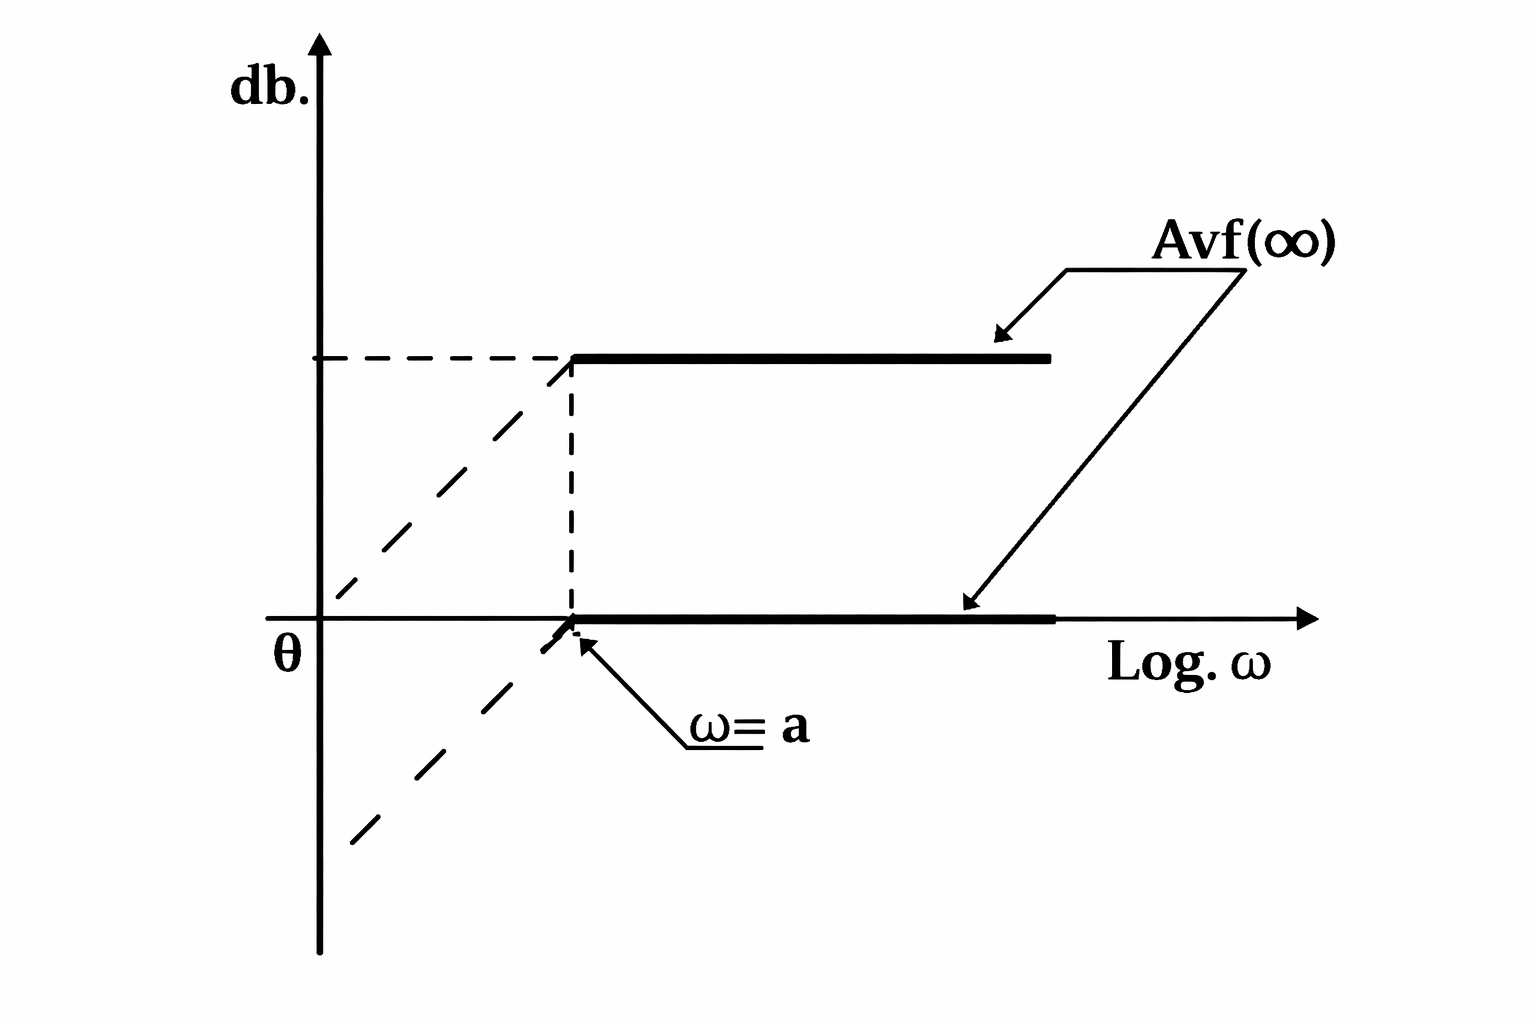
\includegraphics[width=0.5\linewidth]{Imagenes/1.9.png}
    \caption{Respuesta de bode del filtro}
    \label{fig:1.9}
\end{figure}
\subsubsection{Fuentes de corriente}
La Figura~\ref{fig:1.10} muestra una configuración amplificadora que tiene un lazo de realimentación negativa ($R_2$) y otro positivo ($R_1$). Tiene la característica de presentar impedancia negativa en determinadas secciones del mismo (NIC). Esta propiedad se deduce para la impedancia vista hacia la entrada no inversora ($Z^+$). En efecto, teniendo en cuenta que en condiciones ideales las tensiones en ambas resistencias de realimentación son iguales, se obtiene:

\begin{equation}
    \text{Si } v^- = v^+ \implies I_1 \cdot R_1 = -I_2 \cdot R_2 \implies I_2 = I_3 = -\left( \frac{R_1}{R_2} \right) \cdot I_1
    \label{eq:1.10}
\end{equation}

Luego:
\begin{equation}
    Z^+ \cdot I_1 = R_3 \cdot I_3 \implies Z^+ = \left( \frac{I_3}{I_1} \right) \cdot R_3 = -\left( \frac{R_1}{R_2} \right) \cdot R_3
    \label{eq:1.11}
\end{equation}

Intercambiando en la Figura~\ref{fig:1.10} la excitación con $R_3$, se obtiene para la impedancia vista desde la inversora una expresión equivalente:

\begin{equation*}
    Z^- = -\left( \frac{R_2}{R_1} \right) \cdot R_3
\end{equation*}

Ambas muestran una resistencia negativa cuyo valor es una combinación lineal de las conectadas.

Debido a que en el circuito hay realimentación de ambos signos, puede hacerse inestable en el caso de que la neta sea positiva. Esto ocurriría, por ejemplo, en el esquema de la Figura~\ref{fig:1.10} si el nodo no inversor es excitado por una fuente de corriente ideal, debido a que:

\[
K^+ = 1 > K^- = \frac{R_3}{(R_2 + R_3)}
\]

Para revertir esta situación, es necesario que la fuente de excitación tenga una resistencia asociada ($R_4$) de un valor máximo dado por la siguiente relación:

\begin{equation}
    R_4 \le R_3 \cdot \frac{R_1}{R_2}
    \label{eq:1.12}
\end{equation}
\begin{figure}[H]
    \centering
    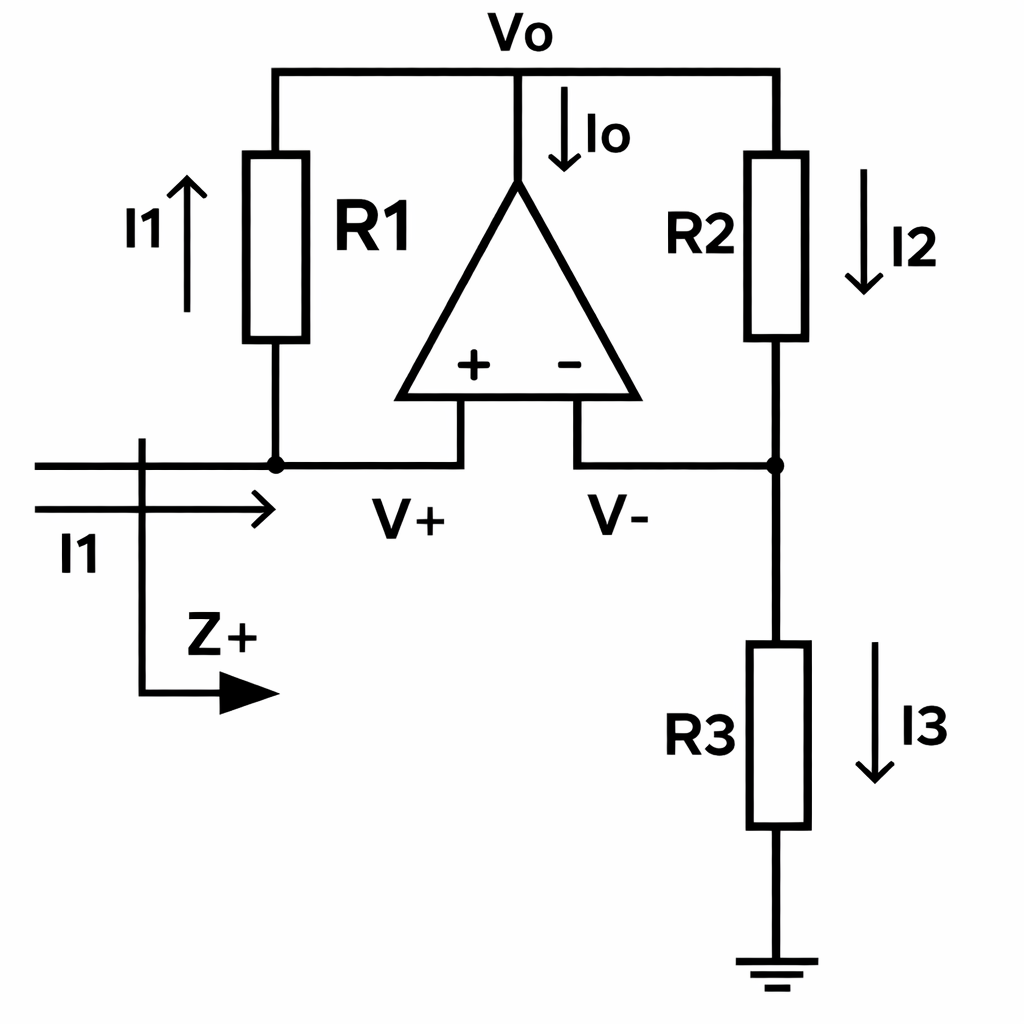
\includegraphics[width=0.5\linewidth]{Imagenes/1.10.png}
    \caption{Conversor a  Inmitancia  Negativa }
    \label{fig:1.10}
\end{figure}
Esta propiedad de convertir una inmitancia real en negativa posee variadas aplicaciones; por ejemplo, permite cancelar el efecto de una resistencia asociada externamente al terminal en cuestión. La Figura~\ref{fig:1.11}a muestra una aplicación que consiste en una fuente de corriente ($I_L$) de impedancia interna infinita controlada por tensión ($V_{in}$), circuito conocido como la bomba de corriente de Howland (desarrollada por B. Howland, M.I.T.).
\begin{figure}[H]
    \centering
    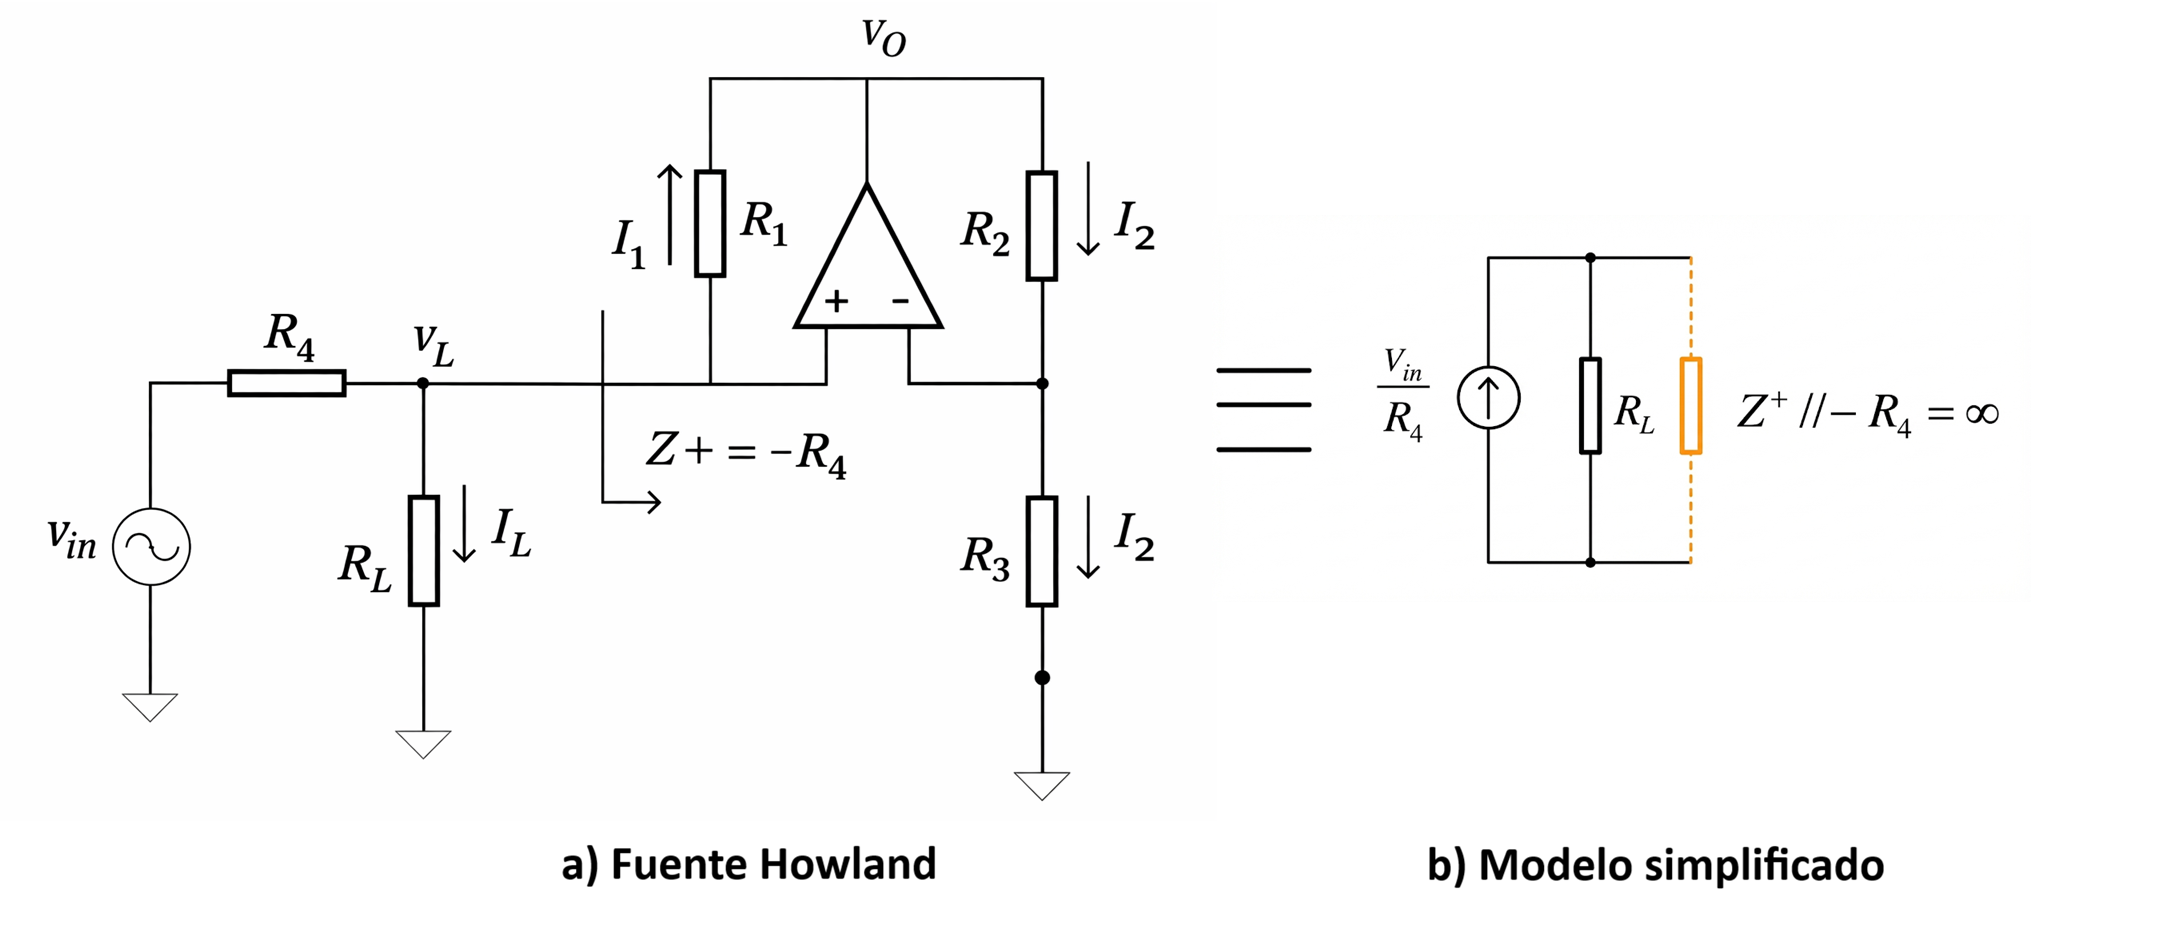
\includegraphics[width=0.95\linewidth]{Imagenes/1.11.png}
    \caption{Simplificación de la fuente Howland}
    \label{fig:1.11}
\end{figure}
Del circuito reducido \eqref{eq:1.11}b, se deduce que si se ajustan adecuadamente los valores dados en \eqref{eq:1.11} se cumple la siguiente relación:

\[
Z^+ = -R_4
\]

Resultando la impedancia vista por la carga de valor infinito, en consecuencia es:
\begin{equation}
    I_L = \frac{V_{in}}{R_4}
    \label{eq:1.13}
\end{equation}

Para ajustar el diseño se deben tener en cuenta las siguientes consideraciones. Por ejemplo, debido a que la tensión de salida del amplificador resulta proporcional a la resistencia de carga \eqref{eq:1.14} y teniendo presente que aquella es inferior a la de alimentación del operacional, la ganancia no inversora que muestra la ecuación de referencia debe bajar, en la medida que aumenta el rango de carga ($R_L$). Esto obliga a reducir $R_2/R_3$ para no exceder $V_{omax}$.

\begin{equation}
    v_o = V^+ \cdot \left( 1 + \frac{R_2}{R_3} \right) = R_L \cdot I_L \cdot \left( 1 + \frac{R_2}{R_3} \right) = \text{Cte.} \cdot R_L \implies R_{Lmax} = \frac{V_{omax}}{\text{Cte.}}
    \label{eq:1.14}
\end{equation}

En consecuencia, un criterio de diseño sería: conocida $V_{omax}$ y la tensión a generar, $V_{Lmax}$, se puede definir la ganancia no inversora máxima y luego con \eqref{eq:1.11} calcular $R_1$.

\[
\frac{V_{omax}}{I_L \cdot R_{Lmax}} \le 1 + \frac{R_2}{R_3} \quad \to \quad R_1 \le R_4 \cdot \frac{R_2}{R_3} \qquad \text{\small (ATENCIÓN: POSIBLE ERROR!)}
\]

Debido a que en un caso de aplicación práctica se deben conectar resistencias comerciales, existirán desviaciones en las relaciones arriba asumidas. En efecto, si se evalúa la impedancia vista por la resistencia de carga en el circuito de la Fig.~1.11b, admitiendo una desviación $\Delta\alpha$ entre los parámetros de ajuste de las relaciones anteriores, se obtiene utilizando \eqref{eq:1.11}:

\begin{equation}
    Z_O = R_4 \, // \, Z^+ = \frac{(1 + \Delta\alpha) \cdot R_4}{\Delta\alpha}
    \label{eq:1.15}
\end{equation}

La anterior muestra que la impedancia interna de la fuente de corriente deja de ser infinita a menos que se corrija la desviación modificando la resistencia adecuada elegida entre las cuatro involucradas.
El esquema (a) de la Figura~\ref{fig:1.12} muestra una fuente de corriente controlada por el modo diferencial de entrada. Dicho esquema puede interpretarse según (b), con el lazo de realimentación positiva abierto y considerando que la impedancia vista desde la sección indicada es mucho mayor que la de carga.
\begin{figure}[H]
    \centering
    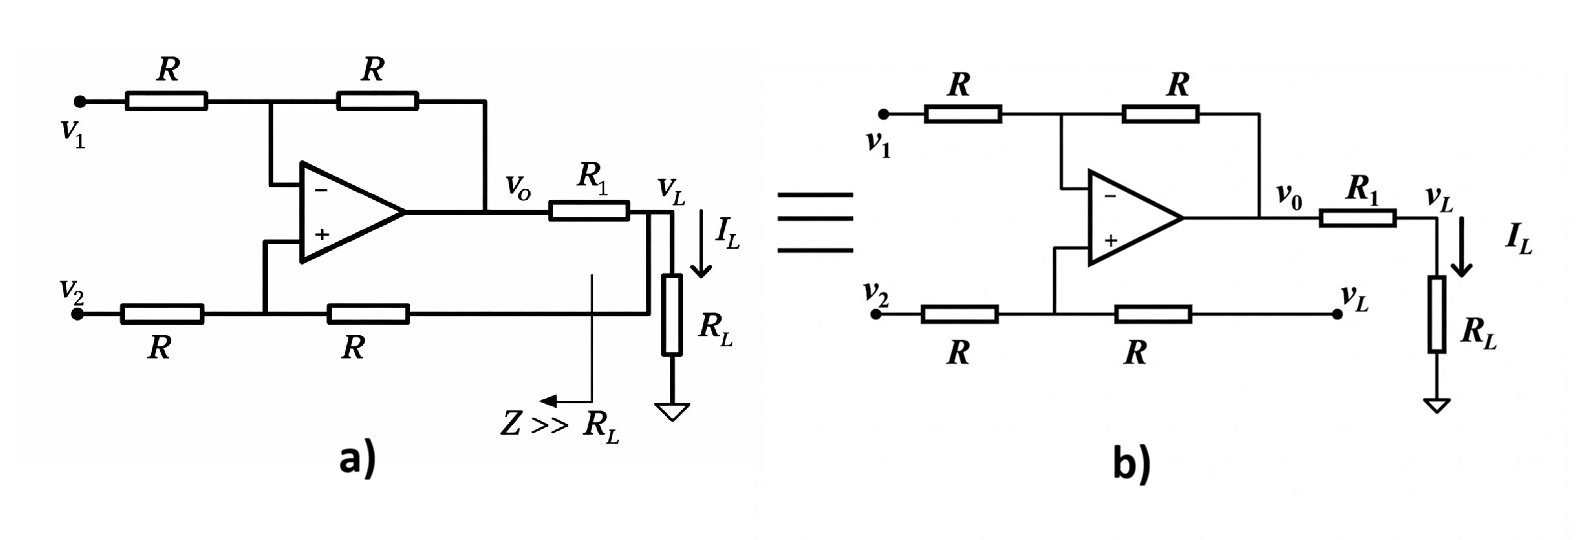
\includegraphics[width=0.85\linewidth]{Imagenes/1.12.png}
    \caption{Fuente de corriente en modo diferencial.}
    \label{fig:1.12}
\end{figure}
Del esquema (b), teniendo presente la conclusión del circuito presentado en E.1, se deducen las siguientes relaciones:

\[
I_L = \frac{v_o - v_L}{R_1} \quad \text{y} \quad v_L = v_o \frac{R_L}{R_1 + R_L} \quad \text{además} \quad v_o = (v_2 - v_1) + v_L
\]

Eliminando $v_o$ de las anteriores se obtiene finalmente:
\begin{equation}
    I_L = \frac{v_2 - v_1}{R_1} = \frac{V_d}{R_1}
\end{equation}

La carga máxima admitida, ($R_{Lmax}$), en operación lineal, de igual manera que en el caso anterior está relacionada con la excursión máxima permitida del AO. En efecto, conocido el modo diferencial máximo aplicado y la corriente de carga requerida, se cumple:

\begin{equation}
    v_{omax} = I_L (R_1 + R_{Lmax})
\end{equation}

Otro parámetro importante del comportamiento de la fuente de corriente es su impedancia interna que puede ser evaluada en el esquema equivalente dado a continuación. En este y en términos ideales se explicita únicamente el lazo que realimenta positivamente al amplificador no inversor de ganancia 2.
\begin{figure}[H]
    \centering
    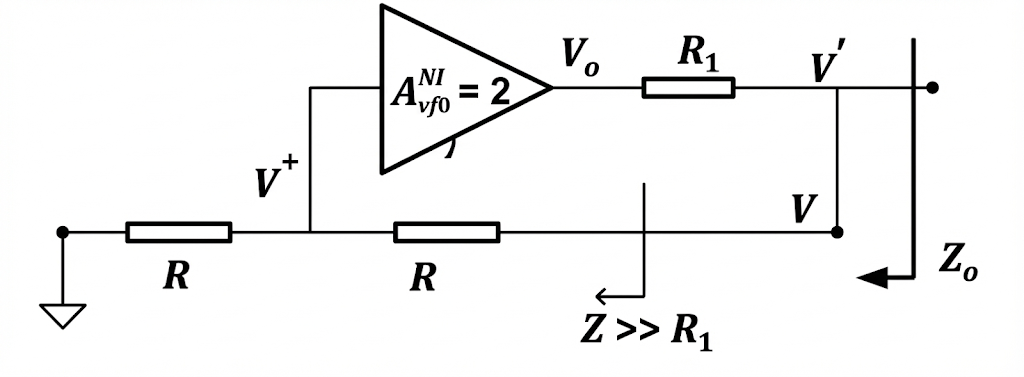
\includegraphics[width=0.5\linewidth]{Imagenes/1.13.png}
    \caption{Impedancia interna}
    \label{fig:1.13}
\end{figure}
Abriendo el lazo en la línea de puntos se deduce, a partir de la expresión de Blackman:

\begin{equation}
    Z_O = R \cdot \frac{1 - T_{CC}}{1 - T_{CA}} \qquad R = \text{Impedancia de sistema muerto, } (v = 0) = R_1
\end{equation}

\[
T_{CC} = \frac{v'}{v} = 0 \quad \text{Debido a que no hay retorno de lazo en la sección de interés } (v' = 0).
\]

En cambio, a sección abierta resulta:

\begin{equation}
    T_{CA} = \frac{v'}{v} = \frac{v^+}{v} \cdot \frac{v'}{v^+} = \frac{1}{2} A_{vfi}^{NI} = +1 \qquad \text{Luego} \qquad Z_0 = \frac{R_1}{1 - 1} = \infty
\end{equation}

Obviamente resulta infinita idealizando el AO; no obstante, en el caso real es finita y de valor muy elevado.
\subsection{Aplicaciones no lineales}
\subsubsection{Amplificador logarítmico}
Obviamente, cuando en la red de realimentación intervienen elementos no lineales activos o pasivos, las relaciones de transferencia resultan no lineales (la salida no es una réplica escalada de la entrada). En términos generales (caso lineal y no lineal), se puede demostrar que cuando en el lazo de realimentación negativa se introduce un bloque funcional definido como $A_f = I_o / V_o$ (Figura~\ref{fig:1.14}), la salida del amplificador realimentado realiza la función inversa, siempre que la función realimentada ($A_f$) no tenga discontinuidades en el rango de operación.
\begin{figure}[H]
    \centering
    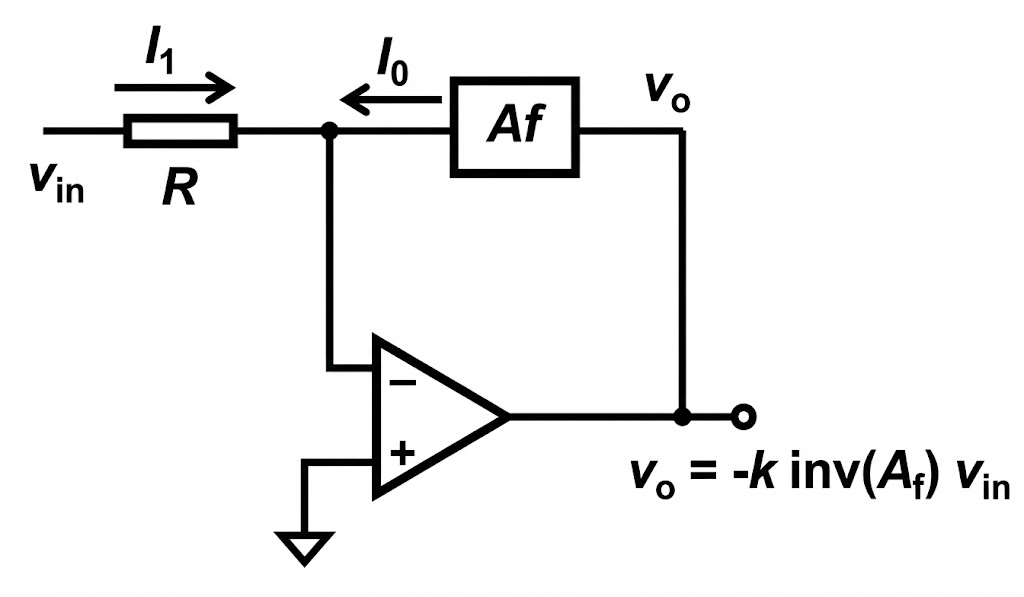
\includegraphics[width=0.5\linewidth]{Imagenes/1.14.png}
    \caption{Amplificador logaritmico}
    \label{fig:1.14}
\end{figure}
Dos casos no lineales típicos son el amplificador logarítmico y los rectificadores de precisión. El primero de ellos se muestra en la Figura~\ref{fig:1.15}, en la cual la tensión de salida se corresponde con la de una junta P-N directamente polarizada (base-emisor). Siendo la relación tensión-corriente exponencial ($I_C \approx I_{S} \cdot e^{k \cdot V_{be}}$), la tensión de salida debería tener una relación inversa (logarítmica) con la corriente inyectada al nudo inversor.
\begin{figure}[H]
    \centering
    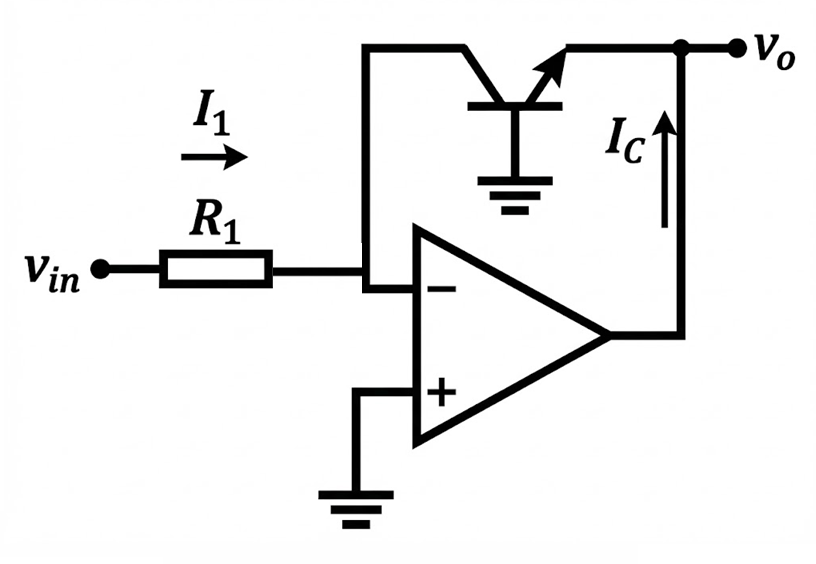
\includegraphics[width=0.5\linewidth]{Imagenes/1.15.png}
    \caption{Modelo de Ebbers-Moll}
    \label{fig:1.15}
\end{figure}
En efecto, el modelo de Ebers-Moll describe el comportamiento de la corriente de colector de un transistor bipolar en términos de la ecuación diódica de Shockley, según la siguiente expresión:

\begin{equation}
    I_C = \alpha_F \cdot I_{ES} \cdot (e^{\frac{V_{BE}}{V_t}} - 1) - I_{CS} \cdot (e^{\frac{V_{BC}}{V_t}} - 1)
    \label{eq:1.16}
\end{equation}

Donde: $V_t = \dfrac{K \cdot T}{q} \cong 26 \text{ mV}$ (T = 300 °K)

Si en el circuito de la Figura 1.13 se cumple que: $A_d \to \infty \implies v_d \to 0 \implies V_{CB} = 0$, la anterior resulta:

\begin{equation}
    I_C = \alpha_F \cdot I_{ES} \cdot (e^{\frac{V_{BE}}{V_t}} - 1) = I_{C0} \cdot (e^{\frac{V_{BE}}{V_t}} - 1)
    \label{eq:1.17}
\end{equation}

$I_{C0} = \text{corriente de saturación inversa de la junta base emisor.}$

Si la junta base emisor es polarizada directamente con tensiones $V_{BE} > 4V_t \cong 100 \text{ mV}$, se puede tomar la corriente de colector en forma simplificada:

\begin{equation}
    I_C \cong I_{C0} \cdot (e^{\frac{V_{BE}}{V_t}})
    \label{eq:1.18}
\end{equation}

Los transistores de señal siguen muy ajustadamente esta ley dentro de un rango de valores de corrientes de colector del orden de 6 décadas (ej: 100 pA $\to$ 100 $\mu$A).

Finalmente, combinando la anterior con las relaciones de corriente del esquema de referencia, se obtiene la siguiente relación logarítmica:

\begin{equation}
    I_1 = \frac{V_{in}}{R_1} = I_C \implies V_o = -V_{BE} = -V_t \cdot \ln \left( \frac{V_{in}}{R_1 \cdot I_{C0}} \right)
    \label{eq:1.19}
\end{equation}

Generalmente, esta salida es invertida por un amplificador de ganancia unitaria.
Es importante analizar los órdenes de magnitud involucrados en la expresión anterior. Por ejemplo, debido a que el valor máximo de la señal de entrada generalmente no supera los diez voltios y el mínimo está limitado por la tensión de offset del amplificador (del orden de los milivolt), el rango dinámico típico de la señal de entrada es de 4 décadas (80 dB). Esto resulta aproximadamente en una excursión de la tensión de salida de:

\[
\Delta V_o \cong 26 \text{ mV} \cdot \ln(10000) = 240 \text{ mV}
\]

Este efecto de compresión de la señal de entrada visto desde la salida es una de las características relevantes del amplificador y es utilizada ampliamente en compresión de datos de señales de video.

Debido a que la expresión \eqref{eq:1.18} es válida siempre y cuando la junta base-emisor tenga polarización directa, la tensión de entrada debe ser siempre positiva, $V_{in} \ge 0$ (Amplificador Logarítmico de un cuadrante).

La relación de transferencia encontrada, vista en un gráfico de escala semi-logarítmica (en base 10), es una línea recta (Fig. 1.16), cuya pendiente es de aproximadamente 60 mV por cada década de variación de la magnitud de la señal de entrada.

\begin{equation}
    \Delta V_o = V_t \cdot \frac{\log(\Delta V_{in})}{\log(e)} = \frac{V_t}{\log(e)} \cdot \log(\Delta V_{in}) \cong 60 \text{ mV} \cdot \log(\Delta V_{in})
\end{equation}
\begin{figure}[H]
    \centering
    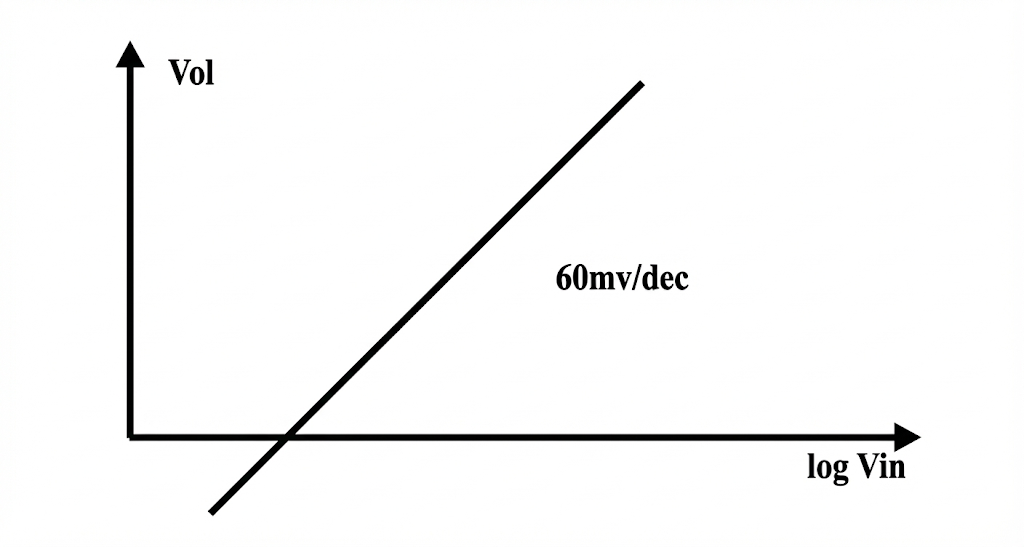
\includegraphics[width=0.5\linewidth]{Imagenes/1.16.png}
    \caption{Relación de transferencia}
    \label{fig:1.16}
\end{figure}
La abscisa al origen de dicha recta es:

\begin{equation}
    V_{in} = I_{C0} \cdot R_1
\end{equation}

La dependencia directa de la pendiente de la relación de transferencia con la temperatura absoluta a través del parámetro $V_t$ y la deriva del cruce por cero debido a la corriente de saturación inversa ($I_{C0}$) ---la cual aproximadamente se duplica cada 10 °C--- se transforman en el talón de Aquiles de esta configuración. 

Ambos problemas tienen variadas soluciones circuitales; una de ellas se muestra en el diagrama en bloques de la Figura~\ref{fig:1.17}, en la que un segundo amplificador logarítmico, idéntico a su homólogo y con ambos transistores térmicamente apareados, es excitado por una tensión muy estable ($V_{ref}$). Su salida ataca la entrada inversora de un amplificador diferencial de ganancia $A$, tal que la relación de transferencia total resulta:

\begin{equation}
    V_o = A \cdot V_t \cdot \ln \left( \frac{V_{in}}{V_{ref}} \right) = A \cdot V_t \cdot \frac{\log \left( \frac{V_{in}}{V_{ref}} \right)}{\log(e)}
    \label{eq:1.20}
\end{equation}

\begin{figure}[H]
    \centering
    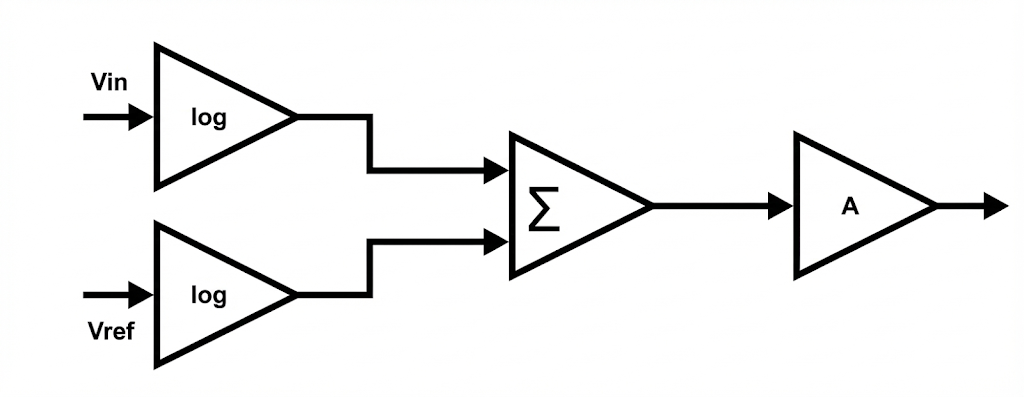
\includegraphics[width=0.5\linewidth]{Imagenes/1.17.png}
    \caption{}
    \label{fig:1.17}
\end{figure}
Esta última muestra que la tensión de cruce queda definida por la tensión de referencia y, además, si la ganancia del amplificador lineal ($A$) se hace dependiente de la temperatura de modo que compense el efecto de $V_t$, también se estabiliza la pendiente ($V_y$).

Intercambiando las posiciones de la resistencia y el transistor mostradas en la Fig.~1.15, se realiza la función inversa (exponencial) Fig.~1.18. En efecto, con los mismos argumentos utilizados en el amplificador logarítmico, se deduce para la tensión de salida la siguiente expresión:

\begin{equation}
    V_o = -I_C \cdot R_2 = -R_2 \cdot I_S \cdot e^{\frac{V_{in}}{V_t}} = V'_{ref} \cdot e^{\frac{V_{in}}{V_t}} \label{eq:1.21}
\end{equation}
\begin{figure}[H]
    \centering
    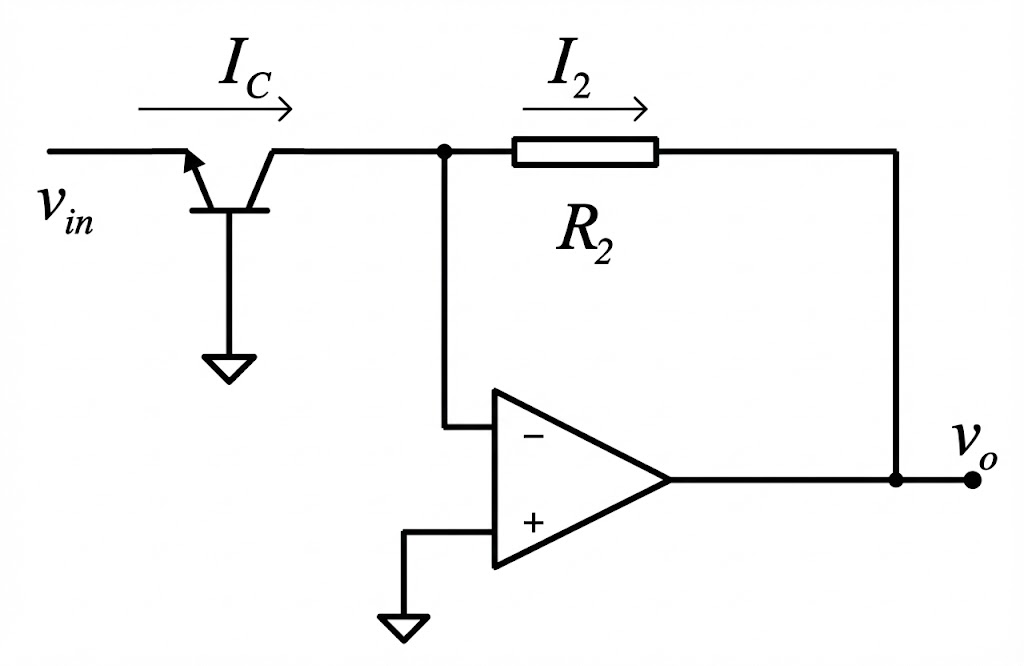
\includegraphics[width=0.5\linewidth]{Imagenes/1.18.png}
    \caption{}
    \label{fig:1.18}
\end{figure}
La relación exponencial de la tensión de salida respecto de la señal de entrada muestra la característica expansora de este amplificador, esto se aprecia mas claramente en una gráfica logarítmica donde la relación de transferencia vuelve a ser una línea recta de pendiente 0.433 $dec/Vt$..

\begin{equation}
\log(V_{0e}) = V_{ref} + \left(\frac{V'_{in}}{Vt}\right).\log(e) \tag{1.22}
\end{equation}

Si la señal de entrada de este amplificador ($V'_{in}$), es la de salida del logarítmico compensado dada en (1.20), ($V'_{in}= V_{0L}$), a partir de la anterior se deduce que la señal de salida ($V_{0e}$), recupera la de entrada ($V_{in}$), a menos de una constante. En efecto en el \underline{log} se verifica que:

\[
V_{0L} = -Vt.Ln\left(\frac{V_{in}}{V_{ref}}\right) \Rightarrow V_{in} = -R_{1}.I_{S}.e^{\left(\frac{V_{0L}}{Vt}\right)}
\]

Comparando la anterior con (1.21) se obtiene para $V'_{in} = V_{0L}$
Una fuente de tensión independiente real, puesta en el lazo, en serie con el generador controlado de salida del O.A., tiene un efecto nulo sobre la tensión de salida en condiciones de operación ideales.

La Figura \ref{fig:1.19}a, muestra un amplificador ideal, excitado por el generador $v_1$ con resistencia interna $r$ que está inserta en el lazo. Para demostrar lo afirmado se analizará en forma independiente el efecto sobre $v_o$ producido por la tensión ($v_1$) y el de $r$ sobre la impedancia vista desde la salida ($r_{of}$).

La \ref{fig:1.19}b muestra el circuito en lazo abierto para evaluar el primero a través de la GLC producida por $v_1$ utilizando la fórmula de Black y para calcular $r_{of}$ mediante la respectiva de Blackman.
\begin{equation}
V_{in} = \left(\frac{R_{1}}{R_{2}}\right).V_{0e} \tag{1.23}
\end{equation}
\subsubsection{Rectificador de precisión}
\begin{figure}[H]
    \centering
    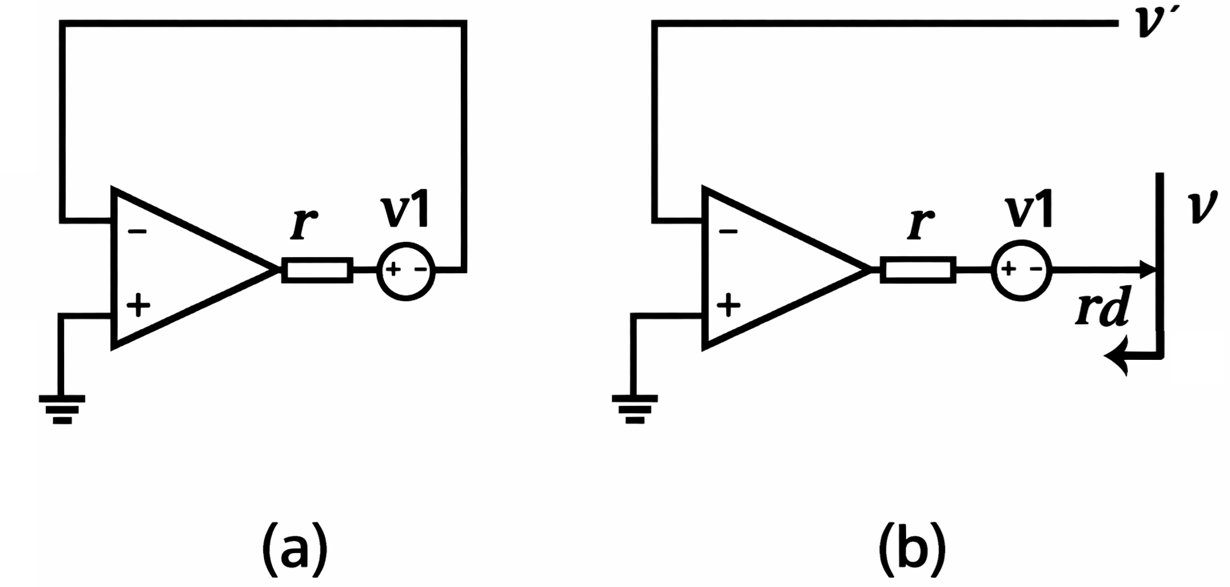
\includegraphics[width=0.5\linewidth]{Imagenes/1.19.png}
    \caption{Realimentacion del amplificador}
    \label{fig:1.19}
\end{figure}
Para el primer caso se deducen las siguientes relaciones para el cálculo de GLC.

\[
\left. G_{LA} \right|_{v=0} = \frac{v_0}{v_1} = -1 \quad \text{y} \quad \left. T \right|_{v_1=0} = \frac{v_0}{v} = -A_d
\]

Luego la ganancia de lazo cerrado es

\begin{equation}
\left. A_{vf} \right|_{A_d \to \infty} = \frac{v_o}{v_1} = \frac{G_{LA}}{(1 - T)} = \frac{-1}{1 + A_d} = 0 \tag{1.24}
\end{equation}

Para el cálculo de la impedancia se deben conocer la del sistema muerto ($r_o$) y las ganancias de lazo con la sección de interés en cortocircuito ($T_{cc}$) y en sección abierta ($T_{ca}$), con los generadores independientes pasivados.

De la figura \ref{fig:1.19}b se deduce además que la impedancia de sistema muerto ($v' = v_I = 0$) es igual a la resistencia interna del generador $v_1$.

\[
r_0 = r
\]

Es fácil ver que la ganancia de lazo, con la sección en cortocircuito es nula

En efecto si: $v_o = 0 \implies T_{cc} = \frac{v'}{v} = 0$
Para el primer caso se deducen las siguientes relaciones para el cálculo de GLC.

\[
\left. G_{LA} \right|_{v=0} = \frac{v_0}{v_1} = -1 \quad \text{y} \quad \left. T \right|_{v_1=0} = \frac{v_0}{v} = -A_d
\]

Luego la ganancia de lazo cerrado es

\begin{equation}
\left. A_{vf} \right|_{A_d \to \infty} = \frac{v_o}{v_1} = \frac{G_{LA}}{(1 - T)} = \frac{-1}{1 + A_d} = 0 \tag{1.24}
\end{equation}

Para el cálculo de la impedancia se deben conocer la del sistema muerto ($r_o$) y las ganancias de lazo con la sección de interés en cortocircuito ($T_{cc}$) y en sección abierta ($T_{ca}$), con los generadores independientes pasivados.

De la \ref{fig:1.19}b se deduce además que la impedancia de sistema muerto ($v' = v_I = 0$) es igual a la resistencia interna del generador $v_1$.

\[
r_0 = r
\]

Es fácil ver que la ganancia de lazo, con la sección en cortocircuito es nula

\[
\text{En efecto si: } v_o = 0 \implies T_{cc} = \frac{v'}{v} = 0
\]

En cambio con la sección en circuito abierto aquella resulta:

\[
T_{ca} = \frac{v'}{v} = -A_d
\]

Finalmente la impedancia en lazo cerrado es:

\begin{equation}
\left. r_{0f} \right|_{A_d \to \infty} = \frac{r_0}{1 - T_{ca}} = \frac{r_0}{1 + A_d} = 0 \tag{1.25}
\end{equation}

Las conclusiones anteriores permiten afirmar, que un diodo puesto en el lazo como indica la \ref{fig:1.20}a, tiene un comportamiento cuasi ideal, permitiendo en consecuencia rectificar con precisión señales del orden de las decenas de microvoltios.
\begin{figure}[H]
    \centering
    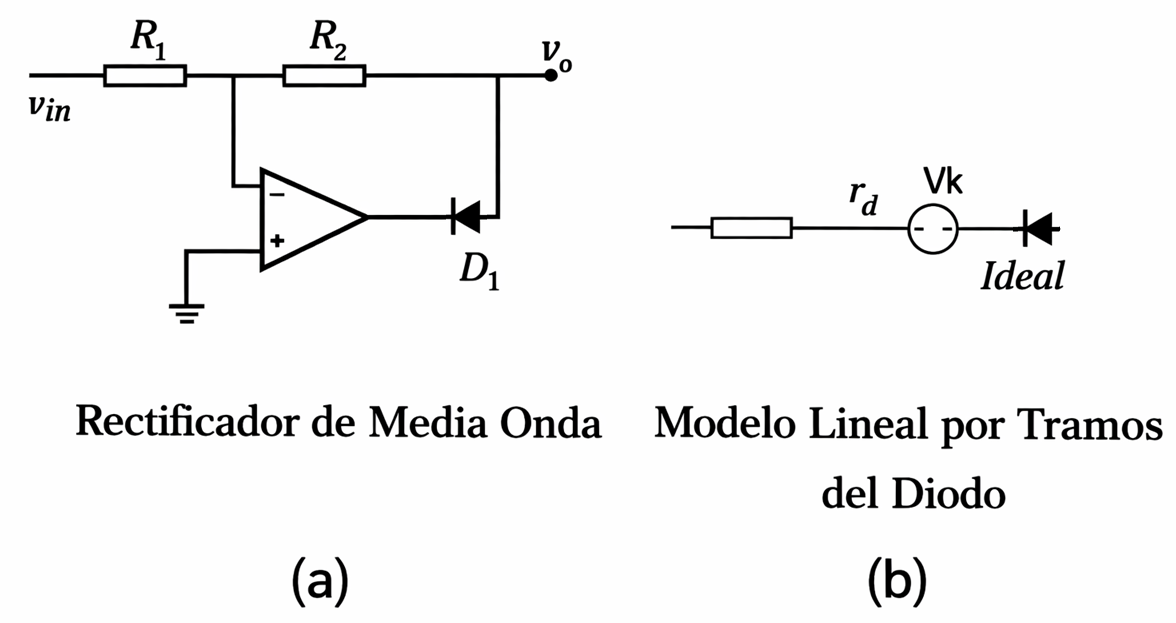
\includegraphics[width=0.5\linewidth]{Imagenes/1.20.png}
    \caption{Modelo lineal del rectificador}
    \label{fig:1.20}
\end{figure}
En efecto si el diodo real es reemplazado por el modelo lineal por tramos de \ref{fig:1.20}b y polarizando directamente el diodo ideal ($v_{in} > 0$), tanto la tensión de codo ($V_K$), como la resistencia dinámica ($r_d$) son reducidas por la ganancia de lazo, según (1.24) y (1.25), tal que en condiciones ideales son anuladas, resultando en consecuencia válido para el semiciclo positivo de la señal.

En cambio en el semiciclo negativo de esta última, el diodo queda polarizado inversamente abriendo el lazo de realimentación respectiva y la salida satura hacia la tensión de alimentación de la barra positiva.

Para evitar esto, se conecta un segundo diodo $D_2$ (\ref{fig:1.21}), que enclava la excursión a $-0.7V$ aproximadamente. Es obvio que invirtiendo la conexión de los diodos de \ref{fig:1.21}, el circuito rectificaría el semiciclo negativo de la señal de entrada.
\begin{figure}[H]
    \centering
    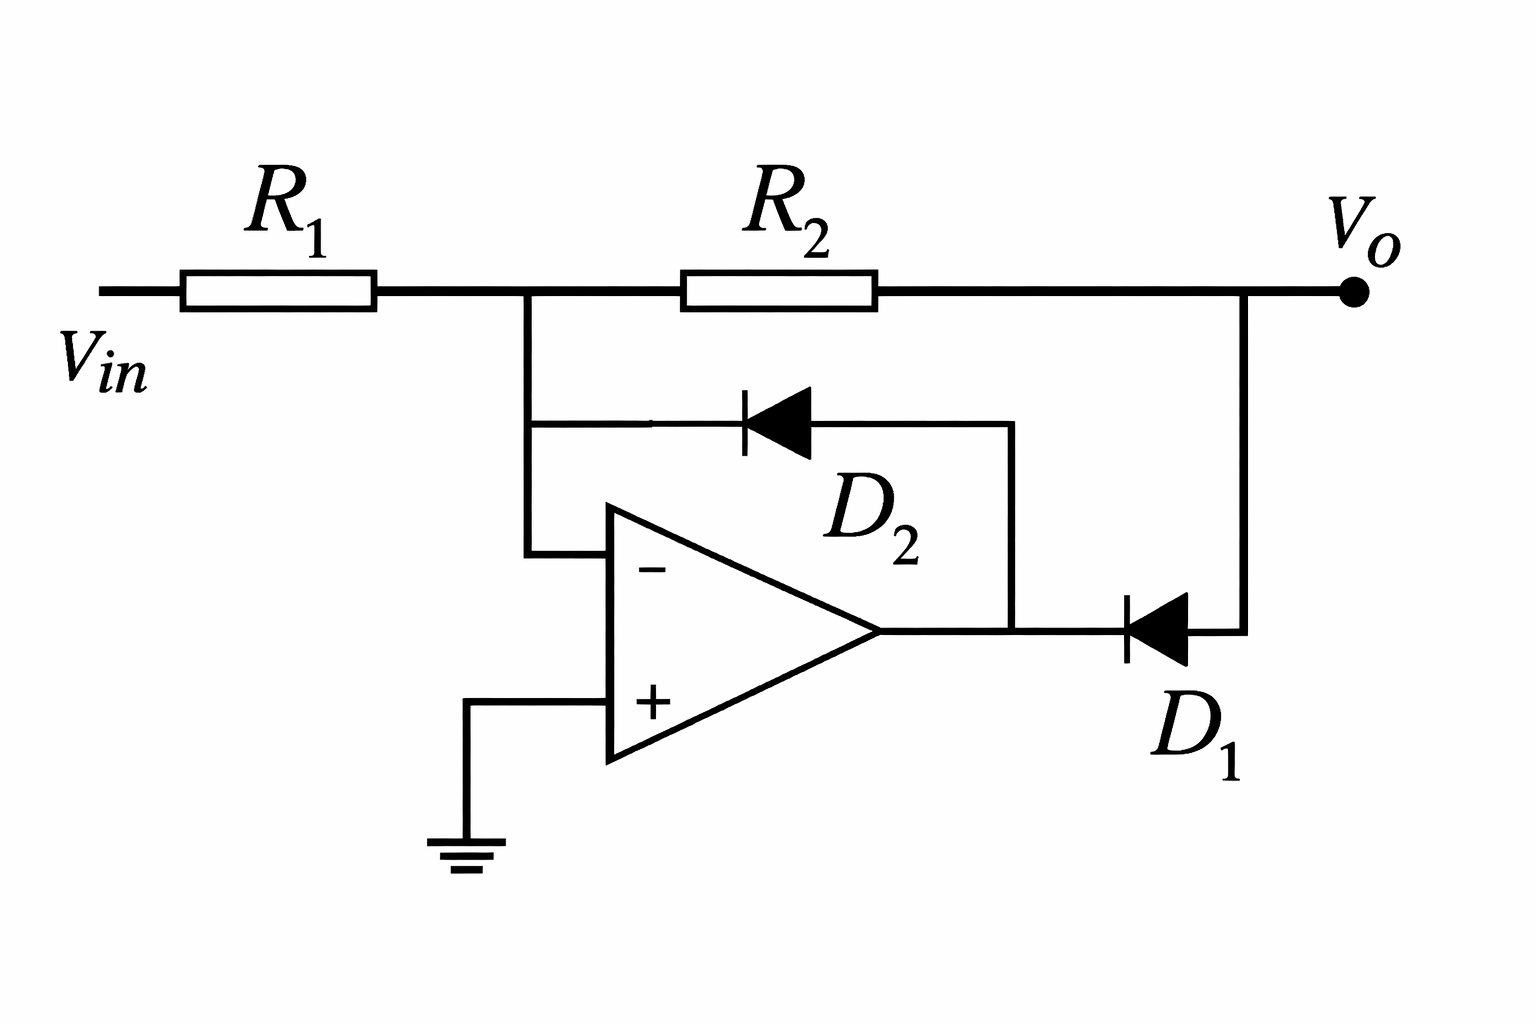
\includegraphics[width=0.5\linewidth]{Imagenes/1.21.png}
    \caption{ Circuito con Enclavamiento }
    \label{fig:1.21}
\end{figure}
No obstante el ejemplo que se analiza a continuación corresponde a una aplicación lineal es oportuno destacar que los conceptos anteriores son aplicables también al diodo base emisor del transistor $Q_n$ y $Q_p$ dentro del lazo de los circuitos de \ref{fig:1.22}.

En efecto, (a) configura una fuente de corriente unipolar controlada por tensión que alimenta la carga $R_L$. El conjunto opera como un amplificador separador (Buffer) con la disponibilidad de corriente de salida del A.O, multiplicada por la ganancia del transistor ($h_{FE}$).

En (b) la conexión configura un amplificador de simetría complementaria en el que debido al comportamiento ideal de las juntas, se elimina la distorsión de cruce, (Clase B ideal), e igual que el caso anterior se aumenta la capacidad de suministro de corriente del A.O a la carga, (Booster de Corriente).

Del esquema (a) se deduce el siguiente valor de la corriente en la carga.

\[
I_L = I_C = \frac{V_{in}}{R_L} \qquad \text{para } v_{in} > 0
\]

De igual manera en (b) para ambas polaridades de la señal de entrada.
\begin{figure}[H]
    \centering
    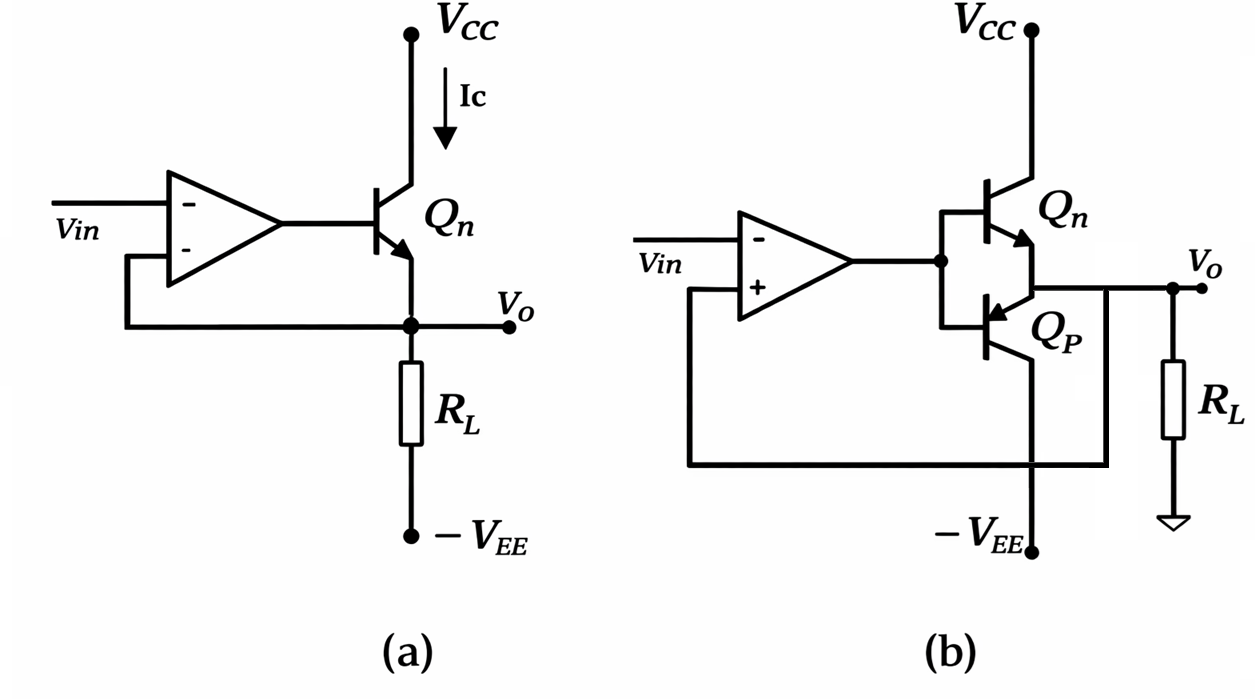
\includegraphics[width=0.5\linewidth]{Imagenes/1.22.png}
    \caption{}
    \label{fig:1.22}
\end{figure}
\subsection{Problemas unidad 1}
\textbf{P.1.1} Calcular las impedancias vistas por el generador de señal y la carga ($z_{in}$, $z_o$), en las configuraciones básicas de \ref{fig:1.5} y \ref{fig:1.6}

\textbf{P.1.2} En el esquema adjunto, el fotodiodo convenientemente iluminado se comporta como una fuente de corriente operando en cortocircuito. El amplificador convierte la corriente del fotodiodo en una tensión proporcional de salida. Deducir la relación de transferencia ideal ($v_o/I_f$) y la impedancia vista por el generador de señal. Considere $r_d = \infty$ y $c_d = 0$.
\begin{figure}[H]
    \centering
    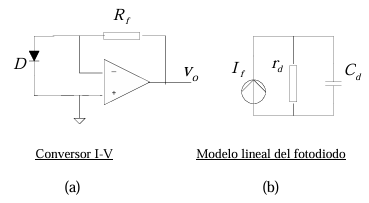
\includegraphics[width=0.5\linewidth]{Imagenes/1.23.png}
    \caption{}
    \label{fig:1.23}
\end{figure}
\textbf{P 1.3} El amplificador diferencial tiene extensa aplicación en acondicionadores de señales analógicas (Instrumentación). Los esquemas siguientes muestran algunas configuraciones típicas y en referencia a ellas desarrollar los siguientes ítems:

\textbf{Config. a)} Encontrar las siguientes relaciones:

\[
v_{o1} = f(v_1, v_2), \quad v_{o2} = f(v_1, v_2), \quad (v_{o2} - v_{o1}) = f(v_1, v_2), \quad \frac{v_{o2} + v_{o1}}{2} = f(v_1, v_2)
\]

\begin{figure}[H]
    \centering
    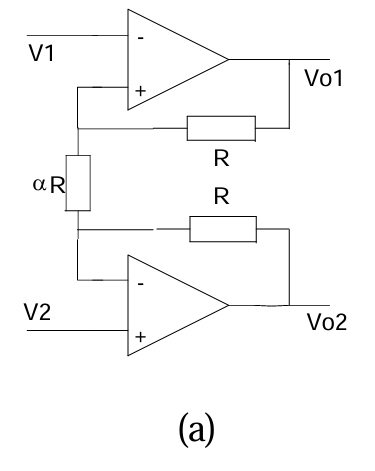
\includegraphics[width=0.5\linewidth]{Imagenes/1.24.png}
    \caption{}
    \label{fig:1.24}
\end{figure}
\textbf{Config. b y c .)} Deducir la ganancia de modo diferencial ($v_o / (v_2 - v_1)$).
\begin{figure}[H]
    \centering
    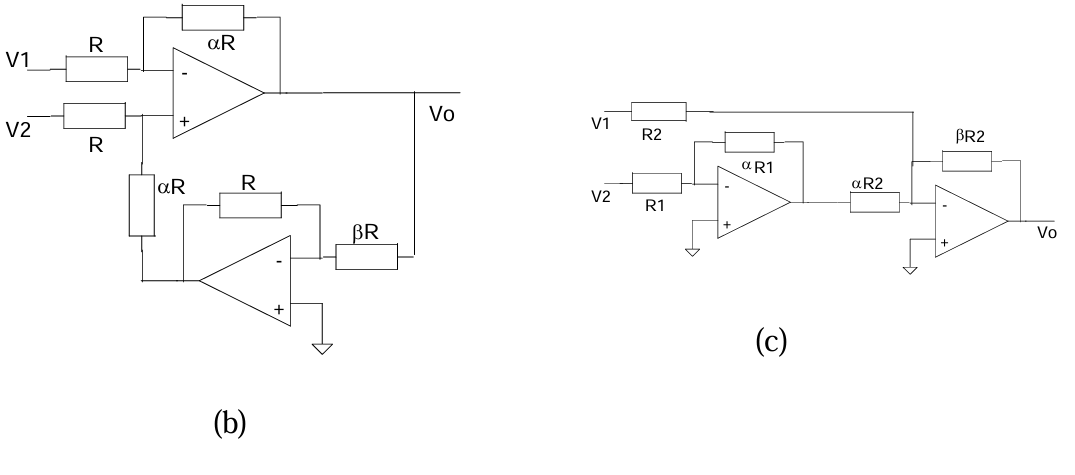
\includegraphics[width=0.85\linewidth]{Imagenes/1.25.png}
    \caption{}
    \label{fig:1.25}
\end{figure}
\textbf{P1.4} Calcular la ganancia de modo diferencial de la configuración resultante de conectar el amplificador de \ref{fig:P1.3}a como excitador del de \ref{fig:1.6}.

\textbf{P.1.5.} Diseñar un amplificador de corriente alterna (\ref{fig:1.7}), con las siguientes características: Ganancia en la banda de paso $(v_o /v_{in}) = -2$, frecuencia de corte en bajas frecuencias $f_L = 1\text{kHz}$.

\textbf{P.1.6.} Diseñar un conversor I-V (\ref{fig:P1.2}) cuyo fondo de escala debe ser de $10\text{V}$ cuando es excitado por un fotodiodo que opera en modo fotovoltaico ($V_d=0$) y debe convertir la corriente mínima de $30\text{pA}$ en $30\mu\text{V}$.

\textbf{P.1.7} Determinadas aplicaciones exigen valores de la resistencia de realimentación muy elevadas penalizando severamente su operación. El resultado del problema 1.6, es un ejemplo. Una solución frecuente y práctica es simular la alta impedancia de realimentación requerida, mediante un cuadripolo como el indicado en \ref{fig:P1.7}. Se pide:

\begin{enumerate}
    \item[a)] Deducir la relación de transferencia, $(V_o / I_f)$, del conversor con el reemplazo indicado en la figura respectiva.
    \item[b)] Calcular un juego de valores de las resistencias donde ninguna supere los $100\text{k}\Omega$, para simular el valor calculado en P1.6.
\end{enumerate}
\begin{figure}[H]
    \centering
    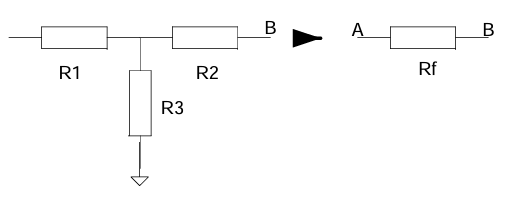
\includegraphics[width=0.5\linewidth]{Imagenes/1.26.png}
    \caption{}
    \label{fig:1.24}
\end{figure}
\textbf{P.1.8.} La fuente de corriente controlada por tensión de \ref{fig:1.11} utiliza el AO-LM324 alimentado por $\pm 10\text{V}$ con los siguientes valores de componentes: $R_1 = R_2 = 10\text{k}\Omega$, $R_3 = R_4 = 600\Omega$, $R_L = 10\text{k}\Omega$, $V_{in} = 25\text{mV}$.

Calcular la tensión en la carga ($R_L$), a la salida del amplificador ($V_o$) y las corrientes circulantes en todas las resistencias para los siguientes valores de la impedancia de carga: $R_L = 0\Omega$; $5\text{k}\Omega$ y $R_{Lmax}$.

Comente los resultados.

\textbf{P.1.9} Si en el problema anterior, el amplificador estuviere alimentado con tensión partida ($\pm 12\text{V}$). ¿Cuál sería el valor de resistencia de carga máxima admitida? Explique.

\textbf{P.1.10} El circuito involucrado en P.1.9 puede funcionar como Óhmetro. Explique.

\textbf{P.1.11} El circuito de la figura es un rectificador de media onda de precisión. Graficar la función de transferencia $V_{out}=f(V_{in})$. En base a lo demostrado en la sección 1.3, considere ideales los diodos.

Sugerencia: analizar separadamente para $V_{in} > 0$ y $V_{in} < 0$.
\begin{figure}[H]
    \centering
    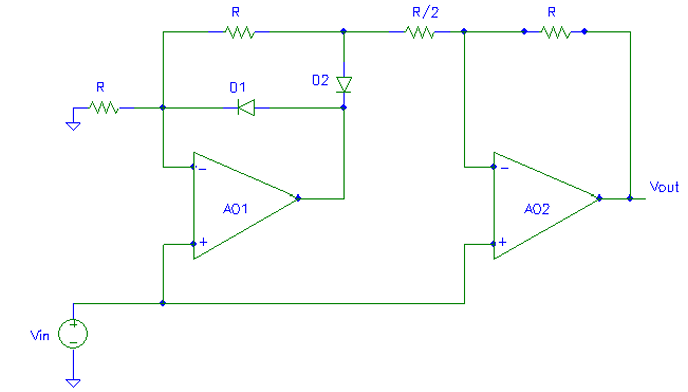
\includegraphics[width=0.5\linewidth]{Imagenes/1.27.png}
    \caption{}
    \label{fig:1.27}
\end{figure}
\textbf{P1.12} Repita el análisis de P1.11, excitando el nodo inversor de $AO_1$, a través de la resistencia $R$.

\textbf{P 1.13} Repita el análisis de P1.12, con el agregado de una resistencia de valor $R$ conectada entre el terminal positivo del generador de señal y la entrada inversora de $AO_2$.

\textbf{P1.14.} El circuito de la figura, opera con ganancia variable por tramos. $AO_1$ es un amplificador operacional ideal. $Z_1$ y $Z_2$ son diodos Zener de $5\text{V}$, $Z_3$ y $Z_4$ de $8\text{V}$. Graficar $V_{out}$ vs $V_{in}$, cuando esta última varía entre $V_{SS}$ y $V_{CC}$. Indicar en el diagrama las coordenadas de los puntos singulares.
\begin{figure}[H]
    \centering
    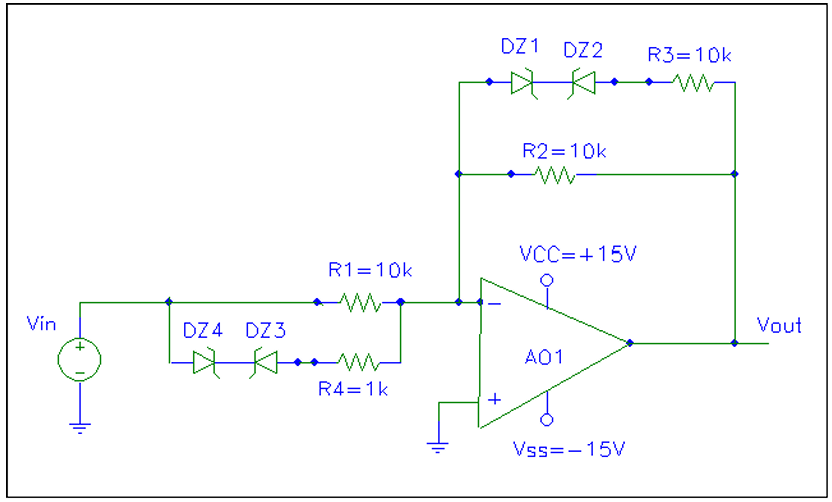
\includegraphics[width=0.5\linewidth]{Imagenes/1.28.png}
    \caption{Enter Caption}
    \label{fig:1.28}
\end{figure}
\newpage
\section{Amplificador real realimentado por tensión}
\subsection*{Introducción}
Los errores miden las desviaciones o rango de incerteza en la determinación de una medida. En el caso de los amplificadores las magnitudes involucradas son señales de tensión, corriente o sus relaciones y las desviaciones respectivas pueden ser expresadas en términos absolutos, (Ej: mV), o relativa al valor máximo que entregaría el amplificador ideal.

No obstante estos conceptos generales, cada sistema adopta modalidades particulares de expresión, por caso si el amplificador evaluado forma parte de una cadena de procesamiento de señal que termina siendo digital es atinente expresar la desviación total de aquel, en número de bits, permitiendo de esta manera coordinar adecuadamente la interfase analógica--digital.

La metodología que se utiliza para analizar y evaluar los efectos de las características reales del amplificador sobre su respuesta, consiste en ponerlos en evidencia de uno en uno idealizando las restantes. Con este procedimiento se evaluarán los errores o desviaciones respecto del comportamiento ideal del conjunto. Por razones didácticas y de uso, es de práctica usual clasificar los errores en estáticos y dinámicos. Los primeros afectan el comportamiento en continua y los segundos están relacionados fundamentalmente con la respuesta en frecuencia.
\subsection{Errores en continua}

Se puede asumir como relevantes a los producidos por las corrientes de polarización ($I_{pol}$), el desajuste de las tensiones de entrada ($V_{OS}$), la ganancia de modo diferencial finita ($A_d$) y la de modo común no nula ($A_c$).

Es necesario aclarar que la expresiones de los efectos de estas magnitudes a la salida (desviaciones) serán particulares para la los amplificadores que se toman como ejemplos, otras estructuras amplificadoras, obviamente propagaran los errores a la salida con expresiones diferentes.

\subsubsection{Efecto de las Corrientes de Polarización de Entrada (Ipol).}

Considerando que las corrientes de polarización no son nulas, la suma de corrientes en el nodo inversor, \ref{fig:2.1} resulta:

\[
i_2 - I_{pol}^- = i_1
\]

De la que se desprende que para minimizar las desviaciones debe ser:

\begin{equation}
i_2 = \frac{v_o - v^-}{R_2} >> I_{pol}^- \tag{2.1}
\end{equation}
\begin{figure}[H]
    \centering
    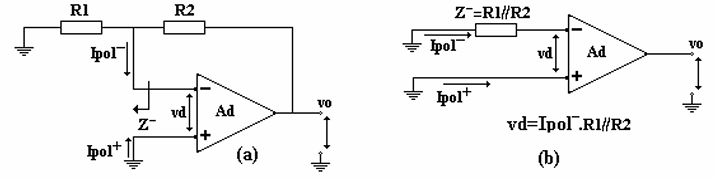
\includegraphics[width=0.5\linewidth]{Imagenes/2.1.png}
    \caption{Corrientes de polarización}
    \label{fig:2.1}
\end{figure}
Es fácil ver en esta última que el desbalance de las impedancias que cargan a ambas, se traduce en un modo diferencial de tensión a la entrada del amplificador que se puede corregir obviamente balanceando aquellas según se muestra en la \ref{fig:2.2}.
\begin{figure}[H]
    \centering
    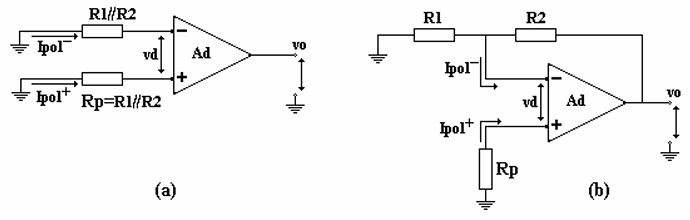
\includegraphics[width=0.5\linewidth]{Imagenes/2.2.png}
    \caption{Corrientes de polarización}
    \label{fig:2.2}
\end{figure}
\noindent La corrección mostrada arriba, anularía la desviación siempre y cuando las corrientes de polarización sean iguales, pero esto no ocurre en la realidad siendo la máxima diferencia el valor $I_{OS}$ ( desajuste de corrientes de entrada), se puede intuir entonces, que la desviación con la solución propuesta será en el peor de los casos proporcional a aquella.

\[
\Delta v_0 \propto I_{pol}^+ - I_{pol}^- = I_{os}
\]

En efecto, de Figura 11b se deduce por superposición.

\[
\Delta v_0 = \Delta v_0 \Big|_{I_{pol}^+ = 0} + \Delta v_0 \Big|_{I_{pol}^- = 0}
\]

\begin{equation} \tag{2.2}
\Delta v_0 = -I_{pol}^- \cdot R_2 + (I_{pol}^+ \cdot R_p) \cdot \left( 1 + \frac{R_2}{R_1} \right)
\end{equation}

\begin{equation} \tag{2.3}
\Delta v_0 = I_{pol}^+ \cdot R_2 - I_{pol}^- \cdot R_2 = \pm I_{os} \cdot R_2
\end{equation}

La desviación mostrada en esta última vuelve a poner en evidencia la proporcionalidad comentada entre la desviación y el valor de la resistencia de realimentación ($R_2$).l
\subsubsection{ Efecto de la Tensión de Desajuste de Entrada (VOS)}
El error producido por el desajuste de la tensión de entrada ($V_{OS}$), se puede evaluar en forma directa reduciendo su efecto a la salida a una señal de modo diferencial equivalente conectada a la entrada según se muestra en la \ref{fig:2.3}, donde el A.O. excitado por el se considera ideal.
\begin{figure}[H]
    \centering
    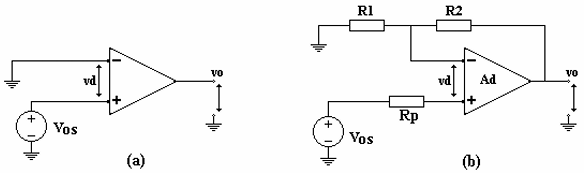
\includegraphics[width=0.5\linewidth]{Imagenes/2.3.png}
    \caption{Tensión de desajuste}
    \label{fig:2.3}
\end{figure}
\noindent En consecuencia tiene la ganancia de un configuración No Inversora Ideal.

\begin{equation} \tag{2.4}
\Delta v_0 = \pm v_{os} \left( 1 + \frac{R_2}{R_1} \right)
\end{equation}

El error total producido por los parámetros analizados, en el peor de los casos puede actuar en el mismo sentido generando un error total:

\begin{equation} \tag{2.5}
\Delta v_0 = \pm \left[ I_{os} \cdot R_2 + v_{os} \left( 1 + \frac{R_2}{R_1} \right) \right]
\end{equation}

El término que dominara en la expresión anterior, depende de la tecnología utilizada y de la calidad del amplificador. En términos generales en aquellos de tecnología (Bi-Fet) o (MOS), es mucho mas importante el producido por la tensión de offset, aunque en tecnología bipolar de precisión pueden ser muy reducido los dos.

Un problema adicional que se presenta es la dependencia de ambos parámetros con la temperatura, esto genera una deriva térmica en la tensión de salida que estará dada:

\begin{equation} \tag{2.6}
\frac{dv_0}{dT} = R_2 \cdot \frac{dI_{os}}{dT} + \frac{dv_{os}}{dT} \cdot \left( 1 + \frac{R_2}{R_1} \right)
\end{equation}

\noindent La manera típica de compensar el efecto de las corrientes de polarización es evitando que, $I_{pol}$, circule por $R_2$ excitando el nodo inversor con una fuente de corriente de igual valor. Figura 2.4, obviamente para evitar la deriva el coeficiente térmico de la corriente de compensación deberá ser igual al de la corriente de polarización, además de estar acoplada térmicamente al amplificador.
\begin{figure}[H]
    \centering
    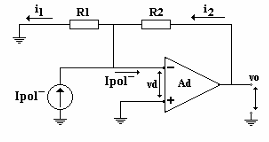
\includegraphics[width=0.5\linewidth]{Imagenes/2.4.png}
    \caption{Tensión de desajuste de entrada}
    \label{fig:2.4}
\end{figure}
\subsubsection{Efecto de la Ganancia de Lazo Abierto  (Ad, Ac)}

\noindent Se denominan de esta manera a las desviaciones de la ganancia de lazo cerrado respecto de su valor ideal, producidas por la ganancia de modo diferencial finita y de modo común no nula.

Para poner en evidencia estos errores, conocidos también como \textit{de ganancia de lazo abierto}, es necesario desarrollar las expresiones de respuesta a partir de la expresión clásica de la ganancia de lazo cerrado del amplificador realimentado (Black ).

\begin{equation} \tag{2.7}
A_{vf}(s) = \frac{A_v(s)}{1 - T(s)}
\end{equation}

\noindent $A_v(s)=$ ganancia de lazo abierto (GLA). \\
$T(s)=$ ganancia de lazo (GL).

\vspace{0.3cm}

Las expresiones anteriores de carácter general pueden ser evaluadas en el circuito de figura 2.5b, del que se deducen las siguientes relaciones particulares para la configuración no inversora.
\begin{figure}[H]
    \centering
    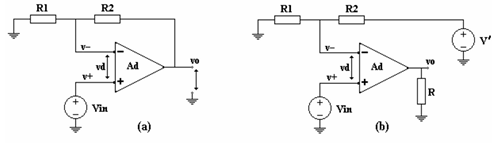
\includegraphics[width=0.5\linewidth]{Imagenes/2.5.png}
    \caption{Ganancia de lazo abierto}
    \label{fig:2.5}
\end{figure}
\noindent En efecto, considerando la ganancia de modo diferencial finita y la de modo común nula, se deduce GLA:

\begin{equation} \tag{2.8}
A_v(s) = \frac{v_0}{v_{in}} \Bigg|_{v'=0} = \frac{v_0}{v_d} \cdot \frac{v_d}{v_{in}} = A_d(s)
\end{equation}

La ganancia de bucle será:

\begin{equation} \tag{2.9}
T(s) = \frac{v_0}{v'} \Bigg|_{v_{in}=0} = \frac{v_0}{v_d} \cdot \frac{v_d}{v'} = -A_d(s) \cdot \frac{R_1}{R_1 + R_2} = -A_d(s) \cdot K
\end{equation}

En base a las relaciones expuestas del amplificador realimentado con ganancia de modo diferencial finita y a los efectos de evaluar los errores producidos, expresaremos la ganancia de lazo cerrado en una forma genérica. Así para el circuito no inversor aquella se puede expresar a partir de (1.7) de la siguiente manera:

\begin{equation} \tag{2.10}
A_{vf}(s) = \frac{A_d(s)}{1 + K \cdot A_d(s)} = \frac{1/K}{1 + \frac{1}{K \cdot A_d(s)}} = \frac{A_{vfi}}{1 - \frac{1}{T(s)}}
\end{equation}

Donde

\[
A_{vfi} = 1 + \frac{R_2}{R_1} \quad \rightarrow \quad GLC \text{ (No inversor ideal)}
\]

Expresando en los mismos términos la correspondiente a una configuración inversora, se obtiene a partir de figura 2.6
\begin{figure}[H]
    \centering
    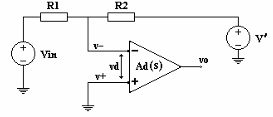
\includegraphics[width=0.5\linewidth]{Imagenes/2.6.png}
    \caption{}
    \label{fig:2.6}
\end{figure}
\noindent Ganancia de lazo abierto:

\begin{equation} \tag{2.11}
A_v(s)\big|_{v'=0} = \frac{v_0}{v_d} \cdot \frac{v_d}{v_{in}} = -A_d(s) \cdot \frac{R_2}{R_1 + R_2} = -A_d(s) \cdot (1 - K)
\end{equation}

En cambio la ganancia de lazo, (independiente del terminal en que se aplica la señal), es igual a la obtenida para la configuración no inversora.

\[
T(s)\big|_{v_{in}=0} = \frac{v_0}{v'} = -A_d(s) \cdot \frac{R_1}{R_1 + R_2} = -A_d(s) \cdot K
\]

Finalmente, GLC resulta a frecuencia cero:

\begin{equation} \tag{2.12}
A_{vf}(0) = \frac{-A_d(s) (1-k)}{1 + K \cdot A_d(s)} = \frac{ \left( 1 - \frac{1}{K} \right) }{ 1 + \frac{1}{K \cdot A_d(s)} } = \frac{A_{vfi}(0)}{1 - \frac{1}{T(0)}}
\end{equation}

El último término de (2.10) y (2.12) son formalmente iguales y se puede demostrar que otras configuraciones mostraran funciones de transferencia en lazo cerrado idénticas, además si la red de realimentación es dependiente de la frecuencia ($K(s)$) resultará la ganancia de lazo cerrado ideal también dependiente de aquella ($A_{vfi}(s)$). De manera que la expresión en cuestión puede ser asumida como alternativa general de representación de la ganancia de lazo cerrado de un amplificador realimentado, en la que además se aprecia claramente que el segundo término del denominador es el causante de la desviación del valor real de la ganancia respecto de su valor ideal. La Figura 2.7 muestra en términos de módulos, las relaciones de respuesta en frecuencia de aquella, en la que se indican los dos tipos de errores que se definen debido a la ganancia de lazo abierto finita, error de ganancia en continua $\epsilon_{G(0)}$ y dinámico $\epsilon_{G(\omega)}$.
\begin{figure}[H]
    \centering
    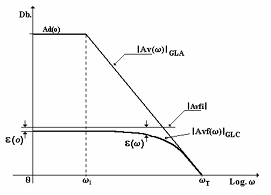
\includegraphics[width=0.5\linewidth]{Imagenes/2.7.png}
    \caption{}
    \label{fig:2.7}
\end{figure}
\noindent Ambos errores se evalúan a partir de la expresión generalizada de GLC, resultando a frecuencia cero según la expresión siguiente.

\begin{equation} \tag{2.13}
\varepsilon_{G(0)} = \frac{1}{T_0}
\end{equation}

En efecto esto se demostrará a continuación. Recordando que la ganancia de lazo ($T$) es negativa y mucho mayor que uno particularmente a frecuencia cero, se puede usar la siguiente aproximación de (2.12):

\begin{equation} \tag{2.14}
\frac{1}{1 + \varepsilon_{G(0)}} \cong 1 - \varepsilon_{G(0)}
\end{equation}

Que permite expresar aquella como:

\[
A_{vf}(0) = A_{vfi}(0) \cdot (1 - \varepsilon_{G(0)})
\]

\[
\varepsilon_{G(Ad)} = \frac{1}{T_0} = \frac{(A_{vfi}(0) - A_{vf}(0))}{A_{vfi}(0)} = \frac{\Delta A_{vf}(0)}{A_{vfi}(0)}
\]

La anterior define a $\varepsilon_{G(0)}$ , como error relativo al ideal producido por la ganancia de lazo finita, que puede ser expresado en términos absolutos según se muestra a continuación

\begin{equation} \tag{2.15}
\varepsilon_{G(Ad)} = \frac{(v_{0i} - v_{0r})}{v_{0i}} = \frac{\Delta v_0}{v_{0i}} \quad \rightarrow \quad \Delta v_0 = \varepsilon_{G(Ad)} \cdot v_{0i} \quad \text{[Volts]}
\end{equation}
\noindent De esta última se deduce, en condiciones de excitación para máxima excursión de salida (Fondo de escala, F.E), la siguiente expresión para la desviación absoluta producida por la ganancia de modo diferencial finita.

\begin{equation} \tag{2.16}
\Delta v_0 = \varepsilon_{G(Ad)} \cdot v_{0|_{\max}}
\end{equation}

Con respecto al efecto producido por la ganancia de modo común no nula, es necesario resaltar que en las configuraciones inversoras es despreciable, ya que el modo común aplicado en esta a la entrada del Amp. Op es prácticamente cero debido a que el potencial de ambas entradas es virtualmente el de tierra. En cambio por la misma razón en las configuraciones no inversoras y diferenciales en general, el modo común aplicado es el valor de la tensión en la entrada no inversora ($V^+$).

En consecuencia se analizará el error de esta última en una configuración básica. La manera clásica de ponerlo en evidencia es convertirlo en una señal de modo diferencial equivalente reducida a la entrada ($v_{ind}$), tal que amplificada por la ganancia de modo diferencial ($Ad$), produzca una tensión de salida ($v_{od}$), igual a la que produciría la de modo común ($Ac$) con la señal de modo común($v_{inc}$).

Esto es:

\begin{equation} \tag{2.17}
v_{od} = A_d \cdot v_{ind} = v_{oc} = A_c \cdot v_{inc}
\end{equation}

\noindent De la anterior se concluye que el modo diferencial equivalente vale:

\[
v_{ind} = \frac{V_{inc}}{\left( \frac{A_d}{A_c} \right)}
\]

Recordando que la relación de rechazo de modo común (RRMC) se define como la relación de las ganancias de modo diferencial y común, la anterior se puede expresar en esos términos.

\begin{equation} \tag{2.18}
v_{ind} = \frac{V_{inc}}{RRMC}
\end{equation}

A partir de esta conclusión se puede modelar al AO, exento de ganancia de modo común, Fig. 2.8, excitado por el modo diferencial equivalente.
\begin{figure}[H]
    \centering
    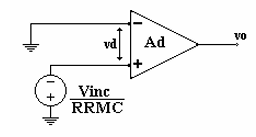
\includegraphics[width=0.5\linewidth]{Imagenes/2.8.png}
    \caption{}
    \label{fig:2.8}
\end{figure}
\noindent Si se realimenta el amplificador anterior, idealizando la ganancia de modo diferencial, que a pesar de ser un contrasentido, (haría la RRMC=$\infty$), permite poner en evidencia únicamente el efecto de la ganancia de modo común.
\begin{figure}[H]
    \centering
    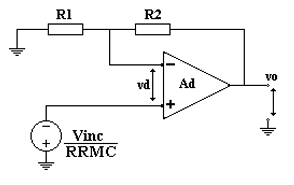
\includegraphics[width=0.5\linewidth]{Imagenes/2.9.png}
    \caption{}
    \label{fig:2.9}
\end{figure}
\noindent En efecto de la anterior se deduce para $Ad = \infty$

\begin{equation} \tag{2.19}
\Delta v_0 = \frac{v_{inc}}{RRMC} \left( 1 + \frac{R_2}{R_1} \right)
\end{equation}

\[
\Delta A_{vf} = \frac{\Delta v_0}{v_{inc}} = \frac{A_{vfi}}{RRMC}
\]

El error relativo resulta

\begin{equation} \tag{2.20}
\frac{\Delta A_{vf}(0)}{A_{vfi}(0)} = \frac{1}{RRMC} = \varepsilon_{G(Ac)}
\end{equation}

Finalmente el error producido por ambas ganancias reales a frecuencia cero es:

\begin{equation} \tag{2.21}
\varepsilon_{G(0)} = \varepsilon_{Ad} + \varepsilon_{Ac} = \frac{1}{T_0} + \frac{1}{\text{RRMC}}
\end{equation}

Cuya desviación absoluta es:

\begin{equation} \tag{2.22}
\Delta v_0 = \varepsilon_{Ad0} \cdot v_{0\text{max}} + \varepsilon_{Ac0} \cdot v_{inc} \cdot A_{vfiN}
\end{equation}

Ambos términos de error expresados en la anterior pueden ser del mismo orden de magnitud, además presentan una significativa dispersión y dependencia con la temperatura. Esta desviación adicional puede ser evaluada en el caso de la ganancia de modo diferencial, a partir de la función sensitividad cuya expresión para grandes variaciones está aproximada en las siguientes expresiones.

\begin{equation} \tag{2.23}
S_{A_d(0)}^{A_{vf}(0)} = \frac{\frac{\Delta A_{vf}(0)}{A_{vf}(0)}}{\frac{\Delta A_d(0)}{A_d(0)}} \cong \frac{1}{1 + K \cdot A_d(0) + K \cdot \Delta A_d(0)}
\end{equation}

El error relativo adicional deducido de está será:

\begin{equation} \tag{2.24}
\varepsilon_0 (\Delta A_d) = \frac{\Delta A_d(0)}{A_d(0)} \cdot S_{A_d(0)}^{A_{vf}(0)} = \frac{\Delta A_d(0)}{A_d(0)} \cdot \left( \frac{1}{1 + K \cdot A_d(0) + K \cdot \Delta A_d(0)} \right)
\end{equation}
\subsubsection{Integración de errores}
\noindent Las desviaciones evaluadas, en el peor de los casos, afectan la salida en el mismo sentido y la desviación total ($\Delta v_{0T}$), puede ser expresada según se comentó, en voltios o en términos relativos al fondo de escala o en número de bits. En este último caso se compara al número de bits que requeriría un conversor A/D, para discriminar dentro del fondo de escala un nivel de tensión equivalente a la desviación total.

\begin{equation}
\Delta v_{0T} \leq \frac{V_{FE}}{2^n}
\end{equation}
\subsection{Respuesta en frecuencia}
\noindent La disminución de la ganancia de lazo abierto con la frecuencia, debido a la presencia de los polos del amplificador básico, adicionan errores que se denominan genéricamente dinámicos. Debido a que la definición y cuantificación de los mismos se efectúa a partir de la respuesta en frecuencia en lazo cerrado de la configuración, es necesario previamente analizar aquella en las configuraciones simples, donde se definirán conceptos y relaciones útiles para tratar formalmente los errores dinámicos relevantes. Se considerará al amplificador básico con ganancia de modo diferencial con un solo polo en la banda de utilización (2.26) y red de realimentación resistiva pura.

\begin{equation} \tag{2.26}
A_d(s) = \frac{A_d(0)}{\left( 1 + \frac{s}{\omega_1} \right)}
\end{equation}

A partir de formula de Black se deduce para la configuración no inversora, la siguiente expresión de GLC.

\begin{equation} \tag{2.27}
A_{vf}(0) = \left[ \frac{A_d(0)}{1 + K.A_d(0)} \right] \cdot \left[ \frac{1}{1 + \frac{s}{\omega_1.(1+K.A_d(0))}} \right] = \frac{A_{vf}(0)}{\left( 1 + \frac{s}{\omega_H} \right)}
\end{equation}

Donde el ancho de banda de 3db está dado por la siguiente expresión:

\begin{equation} \tag{2.28}
\omega_H = \omega_1.(1-T_0) \cong \omega_1.k.A_d(0)
\end{equation}

Tal que el producto ganancia ancho de banda resulta constante:

\begin{equation} \tag{2.29}
GBW = A_{vf}(0).\omega_H = A_d(0).\omega_1 = \omega_T
\end{equation}

La frecuencia de cruce por cero, ($\omega_T$), es un parámetro relevante para la selección del amplificador y es muy útil para la síntesis del mismo, relacionarlo con los requerimientos de ancho de banda y cantidad de realimentación del amplificador realimentado

\begin{equation} \tag{2.30}
\omega_H \cong \omega_1.k A_d(0) = \omega_T.k
\end{equation}

Las magnitudes involucradas en las expresiones anteriores se muestran en el diagrama de módulos de la Figura 2.9
\begin{figure}[H]
    \centering
    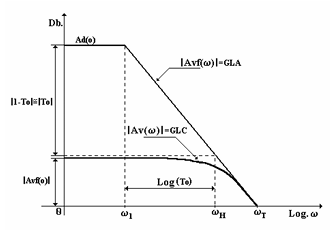
\includegraphics[width=0.5\linewidth]{Imagenes/2.10.png}
    \caption{}
    \label{fig:2.12}
\end{figure}
\noindent Repitiendo el análisis para la configuración inversora, se obtiene:

\begin{equation} \tag{2.31}
A_{vf}(s) = \frac{-A_d(s).(1-K)}{1 + K.A_d(s)} = \frac{-A_d(0).(1-K)}{1 + K.A_d(0)} \cdot \frac{1}{1 + \frac{s}{\omega_1.(1 + K.A_d(0))}}
\end{equation}

\begin{equation} \tag{2.32}
A_{vf}(s) = \frac{A_{vf}(0)}{\left( 1 + \frac{s}{\omega_H} \right)}
\end{equation}

\noindent Donde la ganancia en la banda de paso y el ancho de banda están dados por las siguientes expresiones respectivas

\begin{equation} \tag{2.33}
A_{vf}(0) = \frac{-A_d(0).(1-K)}{1 - T_0}
\end{equation}

\begin{equation} \tag{2.34}
\omega_H \cong \omega_1.k.A_d(0) = \omega_T.k
\end{equation}

\noindent Debe notarse que (2.34), repite la expresión del caso no inversor transformándose en general para amplificadores realimentados con $K$ real y función de transferencia del amplificador con un solo polo.
\begin{figure}[H]
    \centering
    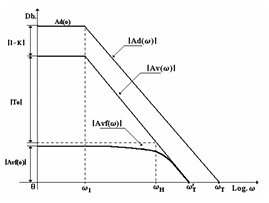
\includegraphics[width=0.5\linewidth]{Imagenes/2.11.png}
    \caption{}
    \label{fig:2.11}
\end{figure}
\noindent A partir de (2.34) debe notarse que la frecuencia de corte de 3 db, ($\omega_H$) será la misma para diferentes configuraciones siempre que tengan idéntica cantidad de realimentación, pero esto implica diferentes ganancias de lazo cerrado ($A_{vfi}=f(K)$), por caso, para los ejemplos analizados NI e IN resultaron:

\[
A_{vfi (NI)} = \frac{1}{K} \quad \text{y} \quad A_{vfi (Inv)} = - \frac{1-K}{K}
\]
Los siguientes ejemplos ilustran el tema.

\noindent \textbf{\large Ejemplo 2.1}

\vspace{0.2cm}

\noindent Demostrar que, si se implementa una configuración NI e IN, de ganancia ideal unitaria, utilizando un A.O con F de T, de un solo polo y frecuencia de cruce $\omega_T$, el inversor tiene la mitad de ancho de banda que el primero.

\vspace{0.3cm}
\hrule
\vspace{0.3cm}

\noindent En efecto:

\[
A_{vfi}\Big|_{NI} = 1 = \frac{1}{K} \Rightarrow k=1 \Rightarrow \omega_H = K.\omega_T = \omega_T
\]

\noindent En cambio para la misma ganancia en configuración inversora será :

\[
A_{vfi}\Big|_{Inv} = -1 = 1 - \frac{1}{K} \Rightarrow K = \frac{1}{2} \Rightarrow \omega_H = \frac{1}{2}.\omega_T
\]

\vspace{0.3cm}
\hrule
\vspace{0.3cm}

\noindent \textbf{\large Ejemplo 2.2}

\vspace{0.2cm}

\noindent A partir del gráfico de fig E.2.2, demostrar que la relación entre las frecuencias de cruce de la ganancia de lazo abierto NI e IN es

\[
\omega'_T = \omega_T.(1-K)
\]

\vspace{0.3cm}
\hrule
\begin{figure}[H]
    \centering
    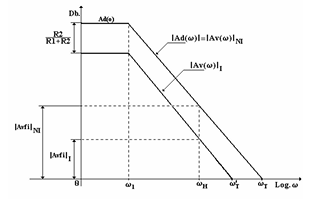
\includegraphics[width=0.5\linewidth]{Imagenes/2.12.png}
    \caption{}
    \label{fig:2.12}
\end{figure}
\noindent \textbf{\large Ejemplo 2.3}

\vspace{0.2cm}

\noindent Analizar la respuesta en frecuencia del amplificador logarítmico.

\vspace{0.3cm}
\hrule
\vspace{0.3cm}

\noindent Es útil analizar la respuesta en frecuencia de aplicaciones amplificadoras realimentadas activamente como lo es por ejemplo el amplificador logarítmico (sección 1.2), debido a que en este caso la ganancia de lazo en continua ($T_0$), puede exceder largamente la de lazo abierto del amplificador básico debido al aporte adicional puesto en el lazo, por el amplificador base común que lo realimenta. Resultando en consecuencia la ganancia de lazo cerrado menor que uno, como se aprecia en el diagrama de módulos E.2.13.

\[
\big| A_{vf}(\omega) \big|_{dB} = \big| GLA(\omega) \big|_{dB} - \big| T(\omega) \big|_{dB}
\]

\noindent En efecto la figura E.2.3.1 muestra al amplificador con el lazo abierto y el transistor reemplazado por su circuito lineal equivalente de baja frecuencia para la conexión base común, del que se deducen las siguientes expresiones.
\begin{figure}[H]
    \centering
    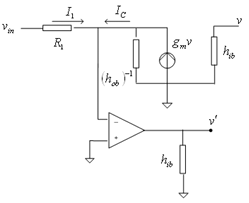
\includegraphics[width=0.5\linewidth]{Imagenes/2.13.png}
    \caption{}
    \label{fig:2.13}
\end{figure}
\[
GLA\big|_{V=0} = - \left( \frac{h_{ob}^{-1}}{R_1 + h_{ob}^{-1}} \right) . A_d(s) \cong A_d(s)
\]

\[
K\big|_{V_{in}=0} = \frac{v'}{v} = gm.R_1
\]

\[
T(s) = \frac{v'}{v} = K.GLA = \frac{-gm.R_1.A_d(0)}{ \left( 1 + \frac{s}{\omega_1} \right) }
\]

\noindent Recordando que: $gm = I_C/V_T$, la ganancia de lazo será proporcional a la corriente de colector y a través de esta de la tensión de entrada, ($I_C=V_{in}/R_1$), tal que a frecuencia cero resulta:

\[
T(0) = - \left( \frac{I_C}{V_t} \right) .R_1.A_d(0) = - \frac{V_{in}}{V_t} . A_d(0) = -K_0 . A_d(0)
\]

\noindent Tomando como ejemplo el VFA OPA627, cuyos datos relevantes son:

\[
A_d(0) = 116dB; \quad f_T = 16MHz \quad \text{y} \quad f_1 = 25Hz
\]

\noindent Para la tensión máxima de señal (10 V), la ganancia de lazo resulta aproximadamente

\[
T(0) = 168 \ dB \Rightarrow \Big| A_{vf}(0) \Big| = -52 \ dB
\]

\noindent Esta dependencia directa de la ganancia de lazo con la amplitud de la señal de entrada, se traslada también al ancho de banda.
\begin{figure}[H]
    \centering
    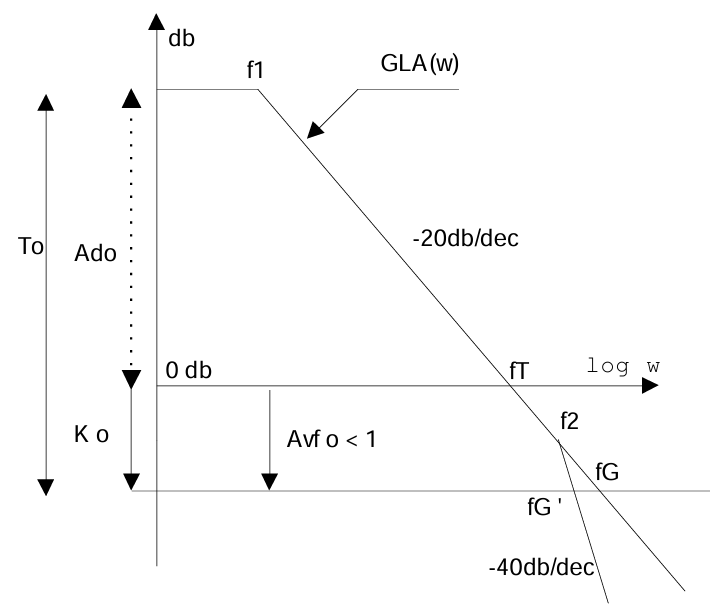
\includegraphics[width=0.5\linewidth]{Imagenes/2.14.png}
    \caption{}
    \label{fig:2.14}
\end{figure}

\[
\omega_H = K.\omega_T = \frac{V_{in}}{V_t}.\omega_T
\]

\noindent Resultando

\noindent $\omega_H = \omega_T$ para $V_{in} = V_t$ y $\omega_H > \omega_T$ para $V_{in} > V_t$

\vspace{0.3cm}

\noindent La dependencia del ancho de banda con la amplitud de la señal, es un problema en este tipo de amplificador, que se agrava sensiblemente si se tiene en cuenta que este generalmente presenta un segundo polo dentro de la década siguiente a la frecuencia de cruce (como muestra en línea de puntos la figuras E.2.3.2), tal que si la frecuencia a que la ganancia de lazo se hace unitaria ($f_{G'}$), es mayor que aquella, el amplificador se tornará inestable.

\vspace{0.5cm}
\hrule
\vspace{0.2cm}

\noindent \textbf{\large Ejemplo 2.4}

\vspace{0.2cm}

\noindent Demostrar que la frecuencia de corte del amplificador diferencial de Fig. 1.6, (Sección 1.1), responde a la expresión dada por (2.34).

\vspace{0.3cm}
\hrule
\vspace{0.3cm}

\noindent Considerando al amplificador con función de transferencia de un solo polo, $A_d(s) = \frac{A_d(0)}{\left( 1 + \frac{s}{\omega_1} \right)}$ y a partir de la expresión de Black, se calculará la ganancia de lazo cerrado desde el circuito siguiente.
\begin{figure}[H]
    \centering
    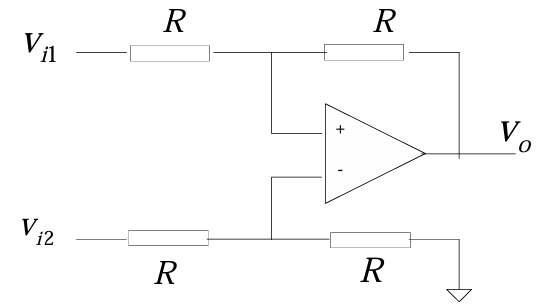
\includegraphics[width=0.5\linewidth]{Imagenes/2.15.png}
    \caption{}
    \label{fig:2.15}
\end{figure}
La ganancia de lazo abierto de cada una de las señales de excitación es:

\[
GLA_1 = \left. \frac{v_o}{v_{i1}} \right|_{v_{i2}=v'=0} = - \frac{R}{R+R} A_d(s) \qquad \text{y} \qquad GLA_2 = \left. \frac{v_o}{v_{i2}} \right|_{v_{i1}=v'=0} = \frac{R}{R+R} A_d(s)
\]

Luego la ganancia de lazo abierto global es:

\[
GLA_1 + GLA_2 = \left. \frac{v_o}{v_{i2} - v_{i1}} \right|_{v,v'=0} = \frac{R}{R+R} . A_d(s)
\]

La ganancia de lazo resulta;

\[
\text{T} = \left. \frac{v_o}{v_i'} \right|_{v_{i1}=v_{i2}=v'=0} = - \frac{R}{R+R} A_d(s) = -k . A_d(s)
\]

Finalmente se resuelve la de lazo cerrado.

\begin{equation}
GLC = \frac{v_o}{v_{i2} - v_{i1}} = \frac{k.A_d(s)}{1 + k.A_d(s)} = \frac{\frac{k.A_d(0)}{(1+s/\omega_1)}}{1 + \frac{k.A_d(0)}{(1+s/\omega_1)}} = \frac{A_{vf}(0)^{Dif1}}{\left( 1 + \frac{s}{\omega_1 . A_d(0) . k} \right)} = \frac{A_{vf}(0)^{Dif1}}{\left( 1 + \frac{s}{\omega_{H1}} \right)} \tag{E.2.4.1}
\end{equation}

En la anterior es

\begin{equation}
A_{vf}(0) = \frac{k.A_d(0)}{1 + k.A_d(0)} \cong \frac{R}{R} = 1 \qquad \text{y} \qquad f_{H1} = k . f_T = \frac{1}{2} f_T = 8 \text{ MHz} \tag{E.2.4.2}
\end{equation}
\hrule
\vspace{1.5mm}
\noindent \textbf{Ejemplo 2.5}
\vspace{1.5mm}
\hrule
\vspace{4mm}
\noindent Calcular el ancho de banda del amplificador del problema 1.3 con los valores dados en el circuito siguiente y utilizando el mismo amplificador VFA que en el ejemplo anterior.
\vspace{4mm}
\hrule
\begin{figure}[H]
    \centering
    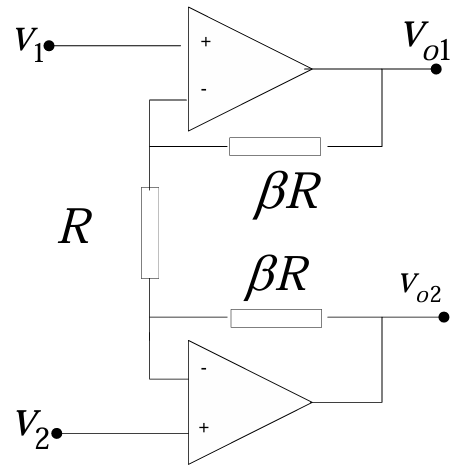
\includegraphics[width=0.5\linewidth]{Imagenes/2.16.png}
    \caption{}
    \label{fig:2.16}
\end{figure}
\noindent Utilizando superposición se deduce por inspección que la salida $v_{01}$ estará conformada por el aporte de $v_1$ con la ganancia no inversora dada por (2.27) y el de $v_2$ con la inversora dada por (2.32).

\[
v_{01} = \left( \frac{A_{vf}(0)^{NI}}{1 + \frac{s}{\omega_{H2}}} \right) v_1 + \left( \frac{A_{vf}(0)^{In}}{1 + \frac{s}{\omega_{H2}}} \right) v_2
\]

\vspace{0.8cm}

\[
v_{02} = \left( \frac{A_{vf}(0)^{NI}}{1 + \frac{s}{\omega_{H2}}} \right) v_2 + \left( \frac{A_{vf}(0)^{In}}{1 + \frac{s}{\omega_{H2}}} \right) v_1
\]

\vspace{0.3cm}

\noindent Con \quad $\omega_{H2} = \omega_1 . A_d(0) . k = \omega_T . k \quad$ y $\quad k = \frac{R}{R + \beta . R} = \frac{1}{1 + \beta}$ \hfill (E.2.51)

\vspace{0.5cm}

\noindent De las anteriores se deduce la ganancia de modo diferencial.

\begin{equation} \tag{E.2.5.2}
v_{02} - v_{01} = \left( \frac{v_2 - v_1}{1 + \frac{s}{\omega_{H2}}} \right) (A_{vf}(0)^{Dif2}) \quad \Rightarrow \quad \frac{v_{02} - v_{01}}{v_2 - v_1} = \frac{A_{vf}(0)^{Dif2}}{1 + \frac{s}{\omega_{H2}}}
\end{equation}

\vspace{0.5cm}

\noindent Finalmente \quad $\omega_{H2} = \left( \frac{1}{11} \right) . \omega_T = 0,09 . \omega_T$
\noindent \textbf{\large Ejemplo 2.6}

\vspace{0.2cm}

\noindent Analizar la respuesta en frecuencia del amplificador que resulta de conectar en cascada el amplificador diferencial del ejemplo 2.4 con el respectivo del ejemplo 2.5, configurando lo que se denomina amplificador de instrumentación.

\vspace{0.4cm}

\noindent En efecto a partir de (E.2.5.2) y (E.2.4.1) se deduce:

\begin{equation*}
\left( \frac{v_{02} - v_{01}}{v_2 - v_1} \right) \cdot \left( \frac{v_0}{v_{02} - v_{01}} \right) = \frac{A_{vf}(0)^{Dif1} \cdot A_{vf}(0)^{Dif2}}{ \left( 1 + \frac{s}{\omega_{H1}} \right) \left( 1 + \frac{s}{\omega_{H2}} \right) }
\end{equation*}

\vspace{0.4cm}

\noindent La anterior muestra una función de transferencia de dos polos, con una separación entre dos y tres octavas. Una primera aproximación manual a la frecuencia de corte de la cascada sería por polo dominante, ($\omega_H \cong \omega_{H1}$) o por suma de las constantes de tiempo respectivas.
\subsubsection{Respuesta en frecuencia}
\noindent Asumiendo el carácter complejo de la GLC dado por cualquiera de sus expresiones matemáticas, se pone en evidencia que los errores a tratar están relacionados con el módulo y fase respectivos o con ambos simultáneamente. Denominándose los dos primeros como de ganancia o \textit{distorsión de frecuencia}, y de fase o \textit{distorsión de retardo} respectivamente.

\begin{equation} \tag{2.35}
A_{vf}(\omega) = \big| A_{vf}(\omega) \big| e^{j \arg(A_{vf}(\omega))}
\end{equation}

\noindent En referencia a la figura 2.12 y asumiendo el carácter de las magnitudes involucradas, se interpreta el error dinámico en términos generales como la diferencia de la tensión de salida ideal y la real a una frecuencia determinada del amplificador realimentado.

\[
\Delta \bar{V}_o = \bar{V}_{oi} - \bar{V}_{o\omega}
\]

\noindent La anterior se expresa en términos relativos, según la siguiente

\begin{equation} \tag{2.36}
\bar{\varepsilon}_\omega = \frac{\Delta \bar{V}_o}{\bar{V}_{oi}} = \frac{\bar{A}_{vfi} - \bar{A}_{vf}(\omega)}{\bar{A}_{vfi}}
\end{equation}

\noindent Teniendo presente la expresión genérica de GLC, (2.12), la (2.36) puede ser expresada de manera compacta

\begin{equation} \tag{2.37}
\bar{\varepsilon}_\omega = \frac{\Delta \bar{V}_o}{\bar{V}_{oi}} = 1 - \frac{\bar{A}_{vf}(\omega)}{\bar{A}_{vfi}} = 1 - \bar{a}_{f(\omega)} = 1 - \frac{1}{1 - \frac{1}{T(\omega)}}
\end{equation}
\begin{figure}[H]
    \centering
    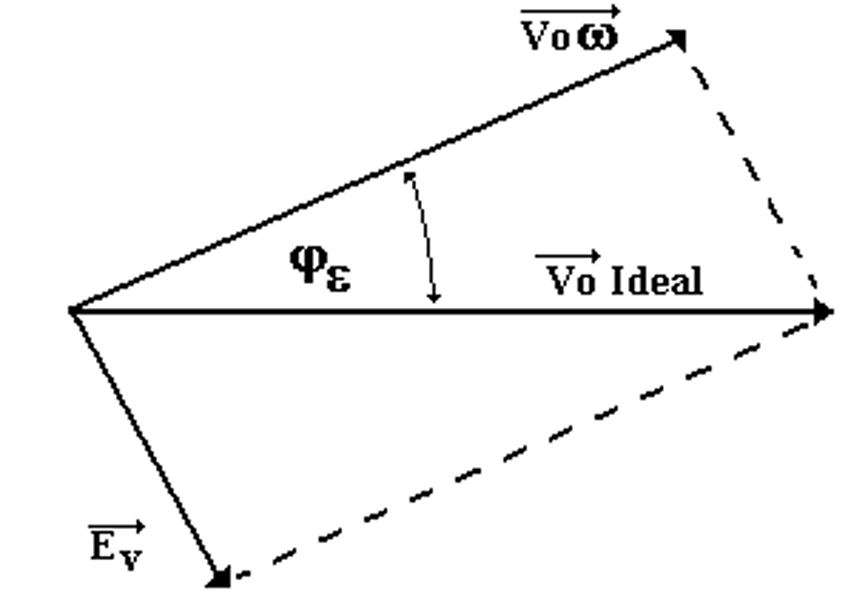
\includegraphics[width=0.5\linewidth]{Imagenes/2.17.png}
    \caption{Enter Caption}
    \label{fig:placeholder}
\end{figure}
\subsubsection{Error vectorial ($\boldsymbol{\varepsilon}_v$)}
\noindent A partir de la ecuación (2.37) se define el error vectorial como el módulo de la diferencia expresada por esta.

\begin{equation} \tag{2.38}
\varepsilon_v = \left| 1 - \frac{1}{1 - \frac{1}{T(\omega)}} \right|
\end{equation}

\noindent Se debe notar que el error vectorial puede ser significativo aun cuando los módulos respectivos no lo sean. La anterior puede expresarse de manera muy simple utilizando la aproximación (2. 14)

\begin{equation} \tag{2.39}
\varepsilon_v = \left| 1 - \frac{1}{1 - \frac{1}{T(\omega)}} \right| = \left| 1 - \left( 1 + \frac{1}{T(\omega)} \right) \right| \cong \left| \frac{1}{T(\omega)} \right|
\end{equation}

\noindent Para \quad $\big| T(\omega) \big| \gg 1$

\vspace{0.3cm}

\noindent Según la anterior el error vectorial puede leerse en decibeles desde el diagrama de módulos de fig 2.13, teniendo presente que son negativos, como corresponde cuando el argumento del logaritmo es menor que uno

\[
\varepsilon_v \big|_{dB} = 1\big|_{dB} - \big| T(\omega) \big|_{dB}
\]

\vspace{0.3cm}

\noindent La expresión (2.39) puede relacionarse con el ancho de banda de 3db ($\omega_H$) y el producto GBW del amplificador, arrojando una ecuación muy práctica para el cálculo manual.

\noindent En efecto teniendo presente que la ganancia de lazo es

\[
T(s) = -k.A_d(s) = \frac{-k.A_d(0)}{\left( 1 + \frac{s}{\omega_1} \right)}
\]

\noindent Se deduce

\begin{equation} \tag{2.40}
\varepsilon_v \cong \left| \frac{1}{T(\omega)} \right| = \left| \frac{1 + j(\omega / \omega_1)}{k.A_d(0)} \right| \cong \frac{1}{T(0)} \cdot \frac{\omega}{\omega_1} = \frac{\omega}{k.A_d(0).\omega_1} = \frac{\omega}{k.\omega_T} = \frac{\omega}{\omega_H}
\end{equation}

\noindent Para $\omega_H \gg \omega$
\begin{figure}[H]
    \centering
    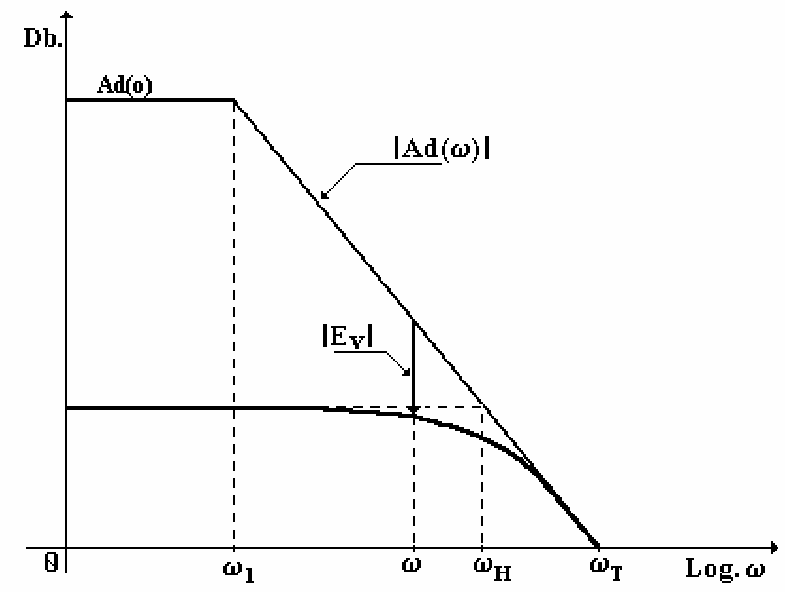
\includegraphics[width=0.5\linewidth]{Imagenes/2.18.png}
    \caption{}
    \label{fig:2.18}
\end{figure}
\subsubsection{Error de Ganancia ($\varepsilon_G(\omega)$)}
\noindent Definido también por \textit{distorsión de frecuencia}, involucra la diferencia de los módulos de los vectores expresados en la ecuación (2.37)

\begin{equation}
    \varepsilon_G = 1 - \left| \frac{1}{1 - \dfrac{1}{T(\omega)}} \right| \cong 1 - \left| 1 + \frac{1}{T(\omega)} \right| \approx 1 - \sqrt{1 + \left( \frac{\omega}{\omega_H} \right)^2} \tag{2.41}
\end{equation}

\vspace{2mm}
\noindent $T(\omega) \gg 1$
\vspace{4mm}

\noindent Al igual que en el caso del error vectorial la anterior puede llevarse a una forma más sencilla utilizando la siguiente aproximación serial para el modulo expresado en ella.

\begin{equation}
    \sqrt{1 + x} \approx 1 + \frac{x}{2} \tag{2.42}
\end{equation}

\noindent $x \ll 1$
\vspace{4mm}

\noindent La (2.41) queda expresada por

\begin{equation}
    \varepsilon_G \cong \frac{1}{2} \left( \frac{\omega}{\omega_H} \right)^2 \tag{2.43}
\end{equation}

\noindent $\omega_H \gg \omega$
\vspace{4mm}

\noindent La manera frecuente de expresar el error de ganancia es como lo muestra la siguiente

\begin{equation}
    (\varepsilon_G)_{Db} = |A_{vfl}|_{Db} - |A_{vf}(\omega)|_{Db} \tag{2.44}
\end{equation}
\noindent De la que se deriva la siguiente

\begin{equation}
|\varepsilon_G|_{Db} = 20 \cdot \log \left( \frac{|A_{vfl}|}{|A_{vf}(\omega)|} \right) \tag{2.45}
\end{equation}

\noindent En esta definición el error evaluado a la frecuencia del codo del diagrama asintótico (Fig. 2.13) es:

\begin{equation*}
\varepsilon_G \big|_{\omega_H} = 3 \text{ dB}
\end{equation*}

\noindent Es de mucha utilidad para el diseño, relacionar el error de ganancia expresado según (2.45) con el producto GBW del amplificador y la ganancia de lazo cerrado ideal.

\noindent Asumiendo que a las frecuencias del extremo superior de la banda se puede considerar:

\begin{equation}
A_{vf(0)} \cong A_{vfl} \tag{2.46}
\end{equation}

\noindent Esto equivale despreciar el error producido por la ganancia no ideal a frecuencia cero. La expresión (2.27), se puede expresar según (2.47).

\begin{equation}
A_{vf}(\omega) = \frac{A_{vf}(0)}{1 + j \dfrac{\omega}{\omega_H}} \cong \frac{A_{vfl}}{1 + j \dfrac{\omega}{\omega_H}} \tag{2.47}
\end{equation}

\noindent La relación de módulos es a partir de esta última.

\begin{equation}
\left| \frac{A_{vfl}}{A_{vf}(\omega)} \right| = \sqrt{1 + \left( \frac{\omega}{\omega_H} \right)^2} \tag{2.48}
\end{equation}

\noindent Además el error dado por (2.45), puede expresarse como:

\begin{equation}
\left| \frac{A_{vf}(\omega)}{A_{vfl}} \right| = 10^{-\frac{\varepsilon_G}{20}} \tag{2.49}
\end{equation}

\noindent Relacionando las anteriores se obtiene finalmente la siguiente:

\begin{equation}
\omega = \omega_H \cdot \sqrt{10^{\frac{\varepsilon_G}{10}} - 1} = K \cdot \omega_T \cdot \sqrt{10^{\frac{\varepsilon_G}{10}} - 1} \tag{2.50}
\end{equation}

\noindent Esta última expresión es muy útil en el proceso de síntesis ya que permite coordinar la ganancia de lazo cerrado ideal, $f(k)$, con el amplificador a utilizar $(\omega_T)$ y la distorsión de frecuencia requerida en $dB, (\varepsilon_G)$, a una frecuencia dada $(\omega)$.
\subsubsection{Errores en la Respuesta para Señales Fuertes}
Es necesario para la comprensión del problema remitirse, aunque con todas las simplificaciones 
posibles, a la estructura interna del amplificador. Por ejemplo el mostrado en Figura 2.14, que re
presenta un caso típico de amplificador VFA. La  primer etapa en configuración diferencial puede 
ser modelada por una fuente de corriente controlada por el modo diferencial de entrada de muy alta 
impedancia de salida (OTA), infinita para el caso, cargada por una de emisor común (Q5 y Q6) de 
muy alta ganancia cuya salida finalmente excita un amplificador separador de ganancia de tensión 
unitaria(Simetría Complementaria).
\begin{figure}[H]
    \centering
    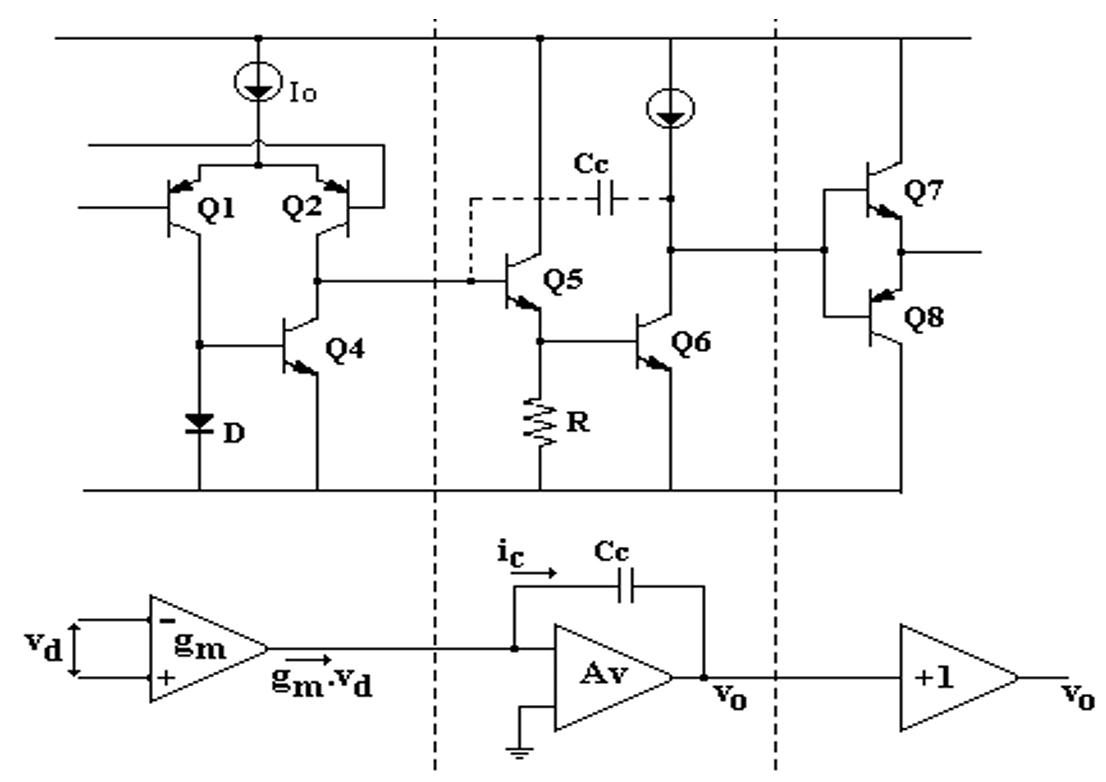
\includegraphics[width=0.5\linewidth]{Imagenes/2.19.png}
    \caption{}
    \label{fig:2.19}
\end{figure}
El amplificador descrito, sin el capacitor Cc conectado, tiene típicamente una función de transferen
cia, para el modo diferencial de entrada con tres polos en la banda de utilización (Fig 2.15).
\begin{figure}[H]
    \centering
    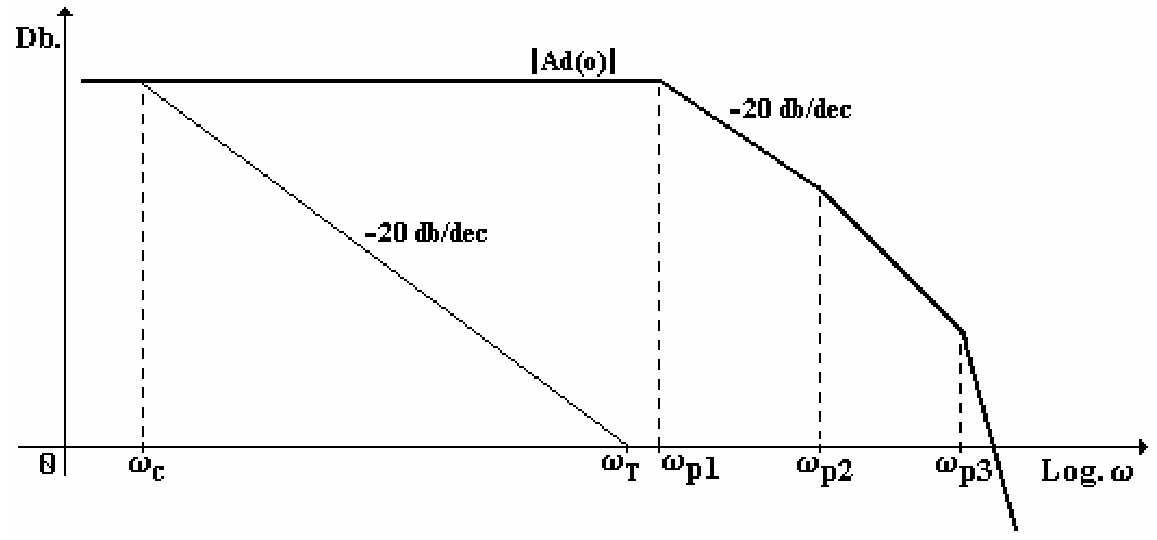
\includegraphics[width=0.5\linewidth]{Imagenes/2.20.png}
    \caption{}
    \label{fig:2.20}
\end{figure}
\noindent Si a un amplificador con este tipo de respuesta se lo realimenta suficientemente presentará problemas de estabilidad. Debido a que en aplicaciones de continua o no muy altas frecuencias, no se requiere un ancho de banda apreciable, el fabricante modifica la característica de respuesta, integrando el capacitor $C_C$ (generalmente de un valor alrededor de los 30pf), a los efectos de generar un polo dominante, ($\omega_C$ en Figura 2.15), en la función de transferencia, tal que el primer polo de la función original ($\omega_{p1}$), quede fuera de la banda de utilización ($\omega_{p1} > \omega_T$). Esta modificación de la respuesta, si bien elimina los potenciales problemas de estabilidad, reduce drásticamente la banda de utilización del mismo para señal débil, hecho que se agrava cuando el amplificador ha de trabajar con grandes excursiones de la tensión de salida. Este último efecto se analizará a continuación.
\begin{figure}[H]
    \centering
    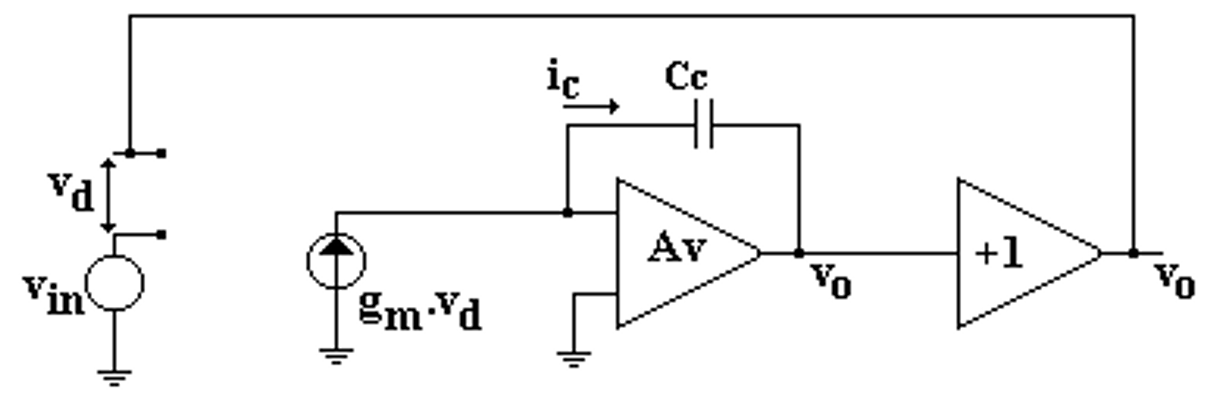
\includegraphics[width=0.5\linewidth]{Imagenes/2.21.png}
    \caption{}
    \label{fig:2.21}
\end{figure}
\noindent Si el amplificador internamente compensado se realimenta negativamente configurando por ejemplo, uno de ganancia unitaria (Buffer). Figura 2.16, se obtiene

\begin{equation} \tag{2.51}
v_0 = v_C
\end{equation}

Y la velocidad de crecimiento de la tensión de salida es

\begin{equation} \tag{2.52}
\frac{dv_0}{dt} = \frac{dv_C}{dt}
\end{equation}

La expresión anterior puede ser puesta en términos de la corriente de señal

\[
C_C \cdot \frac{dv_0}{dt} = C_C \cdot \frac{dv_C}{dt} = i_c = g_m \cdot v_d
\]

Luego

\begin{equation} \tag{2.53}
\frac{dv_0}{dt} = \frac{1}{C_C} \cdot g_m \cdot v_d
\end{equation}

\noindent La anterior muestra que la velocidad de crecimiento de la tensión de salida es proporcional a la corriente de señal disponible a la salida del diferencial, ($g_m \cdot v_d$) y esta tiene como cota superior a la correspondiente a la de polarización de esa etapa ($I_o$), evento que se alcanza cuando el modo diferencial de entrada es cercano al máximo ($v_d \text{ máx}$).

\vspace{0.3cm}

\noindent Se debe recordar que este último es de aproximadamente 100 mV para una etapa diferencial bipolar clásica y del orden del volt, para una de tecnología de efecto de campo.

\vspace{0.3cm}

\noindent Ahora bien, si en el ejemplo que se analiza la señal es débil ($v_{in} \ll v_{d \text{ máx}}$ ), a pesar del retraso de la salida respecto de la entrada (fig. 2.17a) aquella copia la entrada (operación lineal).
\begin{figure}[H]
    \centering
    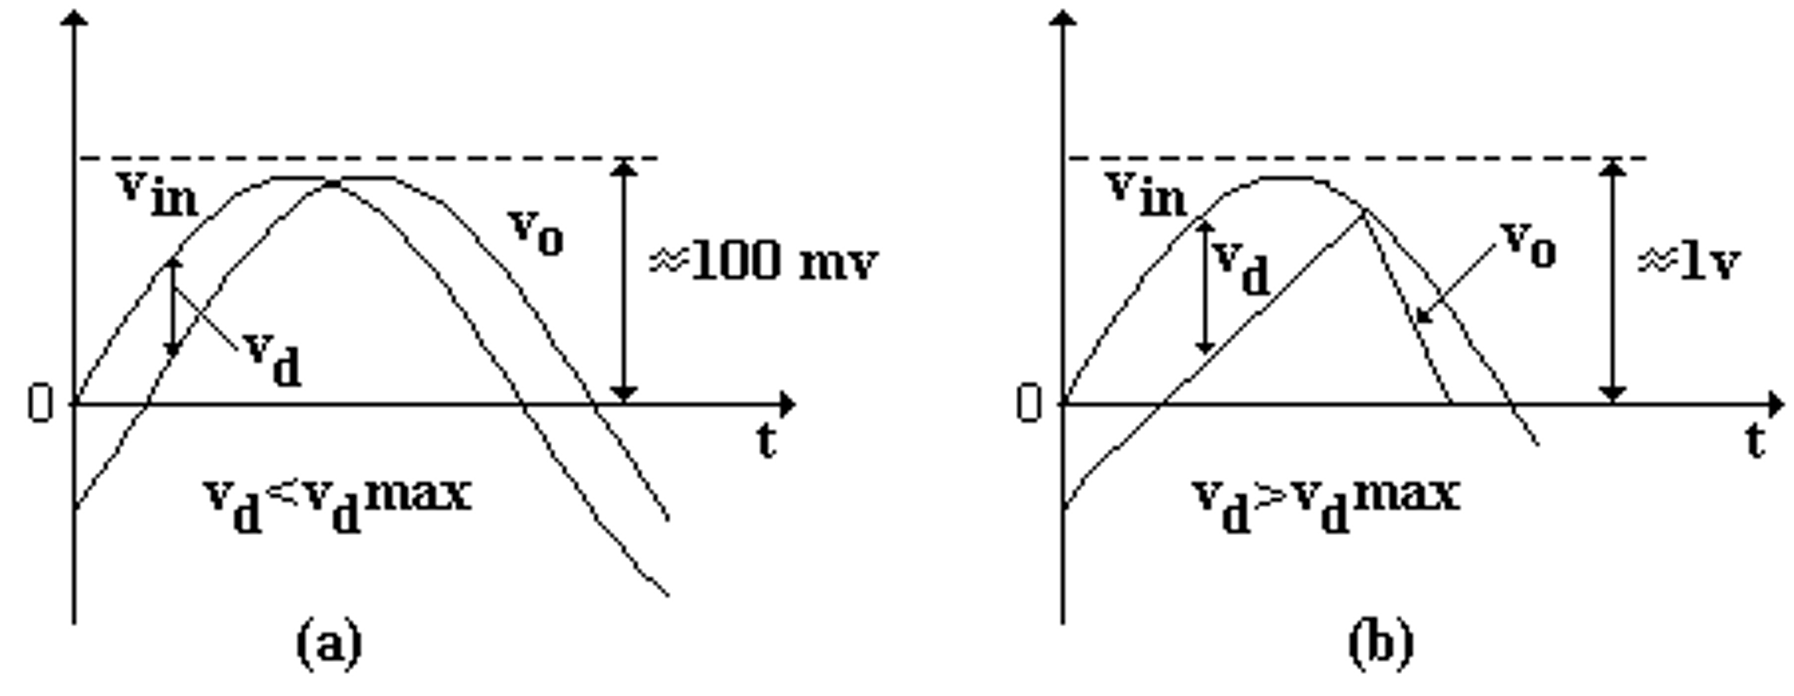
\includegraphics[width=0.5\linewidth]{Imagenes/2.22.png}
    \caption{}
    \label{fig:2.22}
\end{figure}
\noindent Pero si la señal es fuerte (Ej. $v_{in} \ge 1v$) y la velocidad de crecimiento elevada, tal que se llegue a la condición de corriente ($g_m \cdot v_d = I_0$), la tensión de salida varía linealmente ( No puede copiar la entrada, Figura 2.17b). %

\noindent En esta condición la expresión (2.53) queda %

\begin{equation} \tag{2.54}
\frac{dv_0}{dt} \bigg|_{\max} = \frac{I_0}{C_C} = Cte.
\end{equation} %

\noindent La anterior cuantifica el valor máximo que puede tener la velocidad de crecimiento de la tensión de salida, dato que es publicado por el fabricante como \textit{Slew-Rate}. %

\begin{equation} \tag{2.55}
SR = \frac{dv_0}{dt} \bigg|_{\max}
\end{equation} %

\noindent El efecto que produce esta limitación sobre una señal senoidal que ha excedido la condición comentada, se muestra en Figura 2.18. 
\begin{figure}[H]
    \centering
    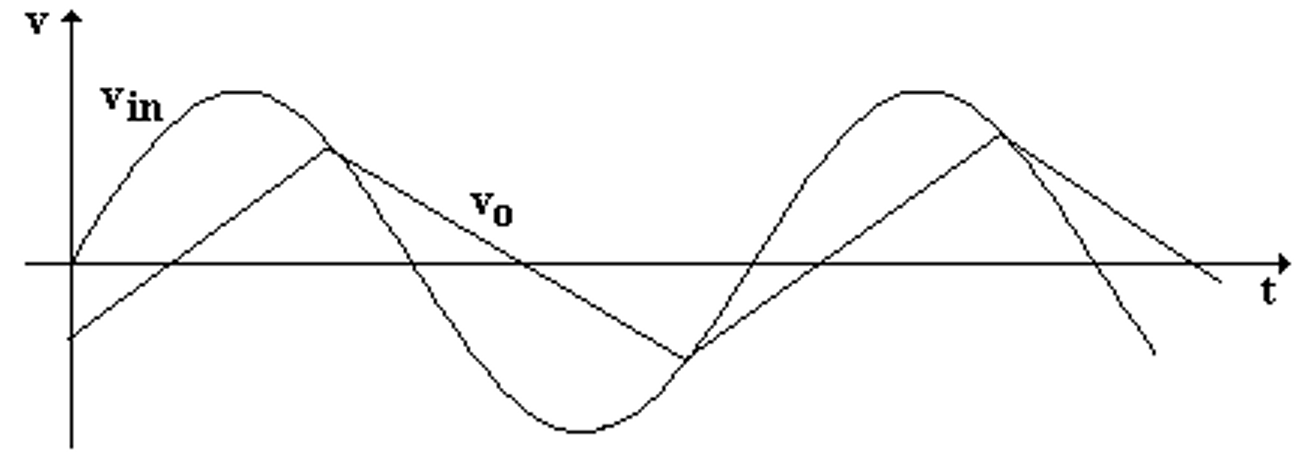
\includegraphics[width=0.5\linewidth]{Imagenes/2.23.png}
    \caption{}
    \label{fig:2.23}
\end{figure}
\subsubsection{Ancho de Banda de Plena Potencia}
\noindent El límite de la velocidad de crecimiento de la tensión de salida, obviamente impone otra cota superior a la respuesta en frecuencia, cuando de grandes excursiones se trata. Este límite se denomina ancho de banda de plena potencia (\textit{Full Power Bandwidth}). Y se define como la máxima frecuencia de una señal senoidal que puede ser reproducida sin distorsión para excursiones de salida elevada (generalmente 10v) se puede demostrar que el ancho de banda de potencia es inversamente proporcional a la amplitud de la señal senoidal.

\vspace{0.3cm}

\noindent En efecto si

\[
v_0 = \hat{v} \cdot \text{sen } \omega \cdot t \quad \rightarrow \quad \frac{dv_0}{dt} = \omega \cdot \hat{v} \cdot \cos \omega \cdot t
\]

\vspace{0.3cm}

\noindent La anteriores máxima para $\cos \omega t = 1$, luego

\begin{equation} \tag{2.56}
\frac{dv_0}{dt} \bigg|_{\max} = SR = \omega_p \cdot \hat{V}_0
\end{equation}

\begin{equation} \tag{2.57}
\omega_{HP} = \frac{SR}{\hat{V}_0}
\end{equation}
\subsection{Problemas unidad 2}
\noindent \textbf{P. 2.1.} Diseñar una configuración no inversora con ganancia $A_{vfi} = 2$ y otra de $A_{vfi} = 200$ ambas con fondo de escala de 5v. Evaluar el error total en continua. Utilizando las siguientes opciones.

\begin{itemize}
    \item[a)] VFA(BIPOLAR) - LM324
    \item[b)] VFA (MOS) – LM6484
\end{itemize}

\noindent \textbf{P. 2.2.} Evaluar el error total para la componente de continua en términos absolutos y relativos a un fondo de escala de 10v, de la tensión de salida del circuito conversor \textit{I-V} del problema P1.6 Utilice las siguientes opciones

\begin{itemize}
    \item[a)] VFA(BIPOLAR) - LM324.
    \item[b)] VFA (FET) - OPA2107
\end{itemize}

\noindent \textbf{P. 2.3.} Analizar el error total propagado a la salida, para la componente de continua en las configuraciones amplificadoras analizadas en P 1.3 y P1.4. Suponga un ajuste perfecto de los valores de las resistencias utilizadas.

\noindent \textbf{P. 2.4.} Diseñar un amplificador diferencial de instrumentación de las siguientes características: Configuración de cuatro AO´s. Rango de excursión de tensión de salida 0-5v con el cero de escala en 2.5v. Ganancia ajustable de 2 a 10 veces. Utilizar el A.O- LM6484. Evaluar el error total a frecuencia cero y verificarlo por simulación en SPICE a $-25^\circ$, $25^\circ$ y $80^\circ$.

\noindent \textbf{P. 2.5} La fórmula de Black, $A_{vf}(s) = A_v(s)/(1-T(s))$, da la expresión de la ganancia de lazo cerrado para un amplificador realimentado y es equivalente a la genérica siguiente $A_{vfi(s)} / (1-(1/T(s)))$. Donde $A_{vfi(s)} = GLC$ (ideal).

\noindent Demuéstrelo para una configuración diferencial simple (fig 1.5), para el conversor I-V del P1.2 y para el amplificador de alterna de Fig 1.7. Suponga al amplificador utilizado con ganancia de modo diferencial con un solo polo $A_{d(S)} = Ad_{(o)} / (1+ s / \omega_1 )$.

\noindent \textbf{P. 2.6.} En el problema P.2.1 el fotodiodo tiene una impedancia interna $r_d = 10 \text{ Megohms}$ y utiliza VFA-LM6484. Dibuje el diagrama de Módulos de GLC, GLA y T. Deduzca el ancho de banda de 3db ($\omega_H$) de la configuración.

\noindent \textbf{P. 2.7} Calcule al ancho de banda de 3db ($\omega_H$) y de 1db, en las configuraciones correspondientes al problema P. 2.4.

\noindent \textbf{P.2.8} El rectificador de precisión del problema P1.12 y 1.13, utiliza el VFA-LM324. Evalúe el ancho de banda de 3db de ambas configuraciones.

\noindent \textbf{P.2.8.} El amplificador de alterna del P.1.5 utiliza el AO-LM324. Dibuje el diagrama de módulos de la respuesta (GLA, GL y GLC).
\newpage
\section{Amplificadores realimentados por corriente (CFA)}
\subsection{Introducción}
Este tipo de amplificador pertenece al grupo de aquellos que para operar linealmente, deben ser realimentados negativamente debido a su elevada ganancia de lazo abierto. No obstante presentan características funcionales dinámicas distintas al operacional clásico (VFA). La diferencia de arquitectura, principalmente de la etapa de entrada y además el menor número de estas, resultan en aumento de velocidad, tanto en pequeña como en gran señal, con rangos de operación superiores a $100\,\text{MHz}$ y más de $1000\,\text{V}/\mu\text{s}$ respectivamente, mostrando producto ganancia ancho de banda del orden del GHz, aunque la precisión en continua es en general más pobre que aquellos.

La figura \ref{fig:3.1} muestra un modelo compacto del amplificador realimentado por corriente también denominado de Transimpedancia, nombre justificado por el hecho que, el generador de tensión de salida está controlado por la corriente de señal de la entrada inversora ($I_{\text{in}}$), terminal este, de muy baja impedancia (ej. $20\,\Omega$), que se corresponde con el de salida del buffer cuya entrada, de muy alta impedancia, configura la no inversora.
\begin{figure}[H]
    \centering
    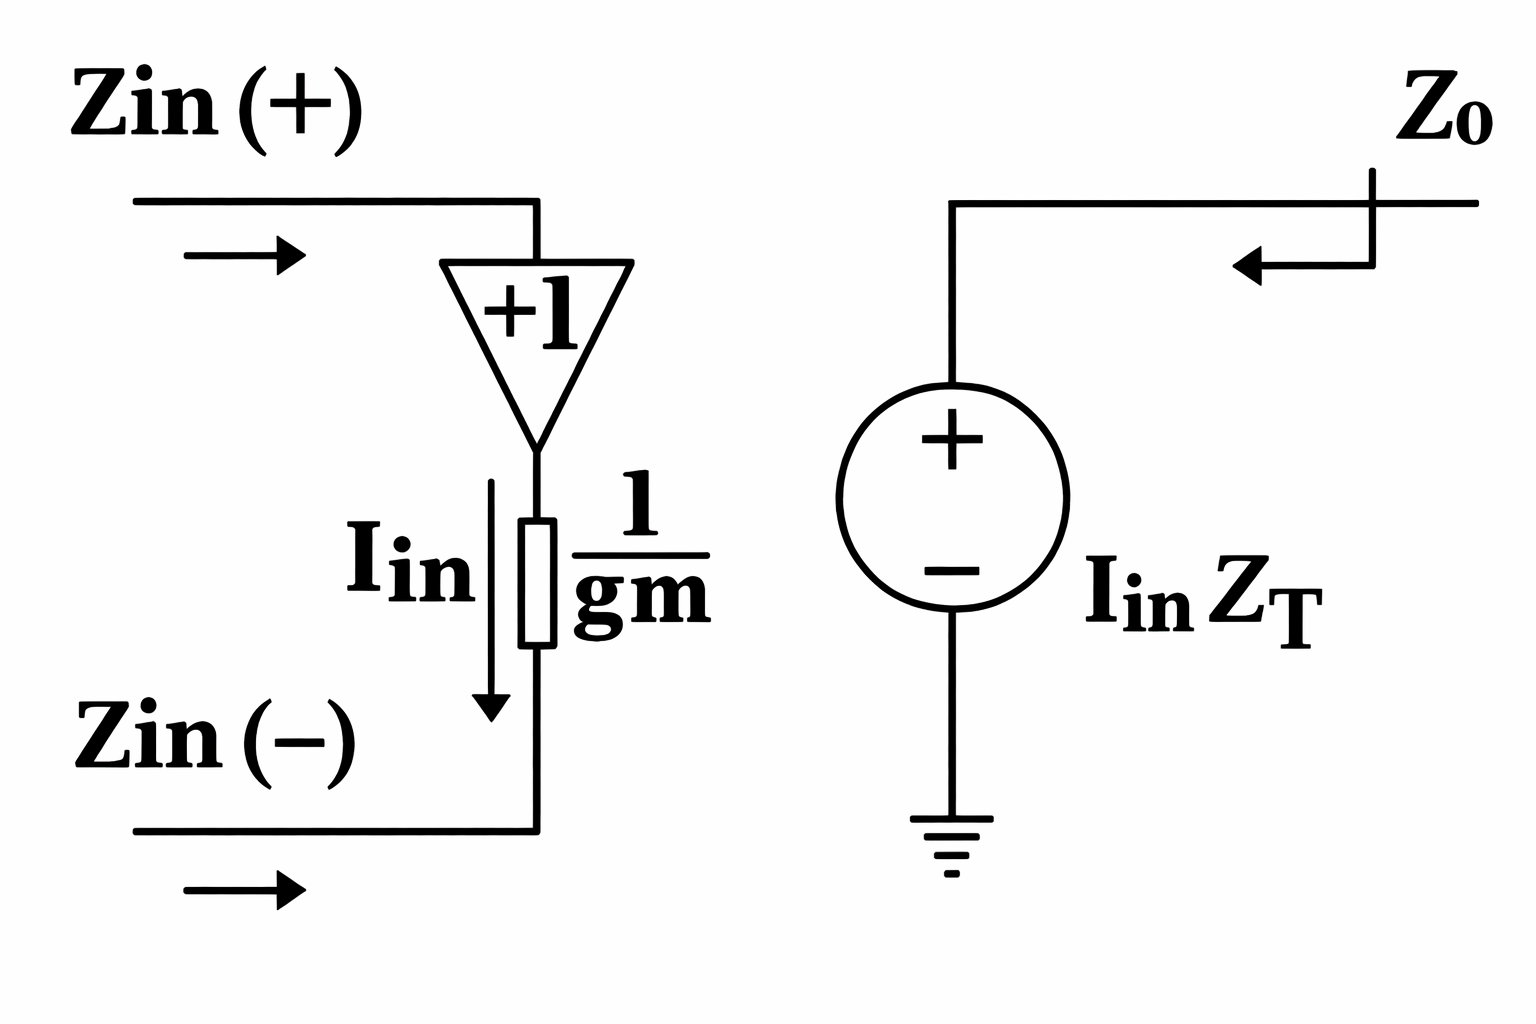
\includegraphics[width=0.5\linewidth]{Imagenes/3.1.png}
    \caption{CFA}
    \label{fig:3.1}
\end{figure}
La transimpedancia $Z_T(s)$, puede ser aproximada en la banda de utilización por una función de transferencia de un solo polo como lo indica (\ref{eq:3.1})

\begin{equation}
Z_t(s) = \frac{R_t}{1 + s R_t C_t}
\label{eq:3.1}
\end{equation}

Donde, $R_t$ y $C_t$ se denominan transresistencia y transcapacitancia respectivamente, con valores típicos en torno al megaohm y los $2\,\text{pF}$ respectivamente. La transimpedancia es publicada en hojas de dato, en diagramas de módulo y fase, mostrando esta última polos de segundo orden cuyo, efecto sobre la respuesta será analizado posteriormente en temas relativos a la estabilidad del amplificador. A continuación se analizará la respuesta de las configuraciones típicas.
\subsection{Respuesta en frecuencia}
Se evaluará  la respuesta del amplificador en la configuración no inversora de (\ref{fig:3.2}), idealizando el 
Buffer de entrada
\begin{figure}[H]
    \centering
    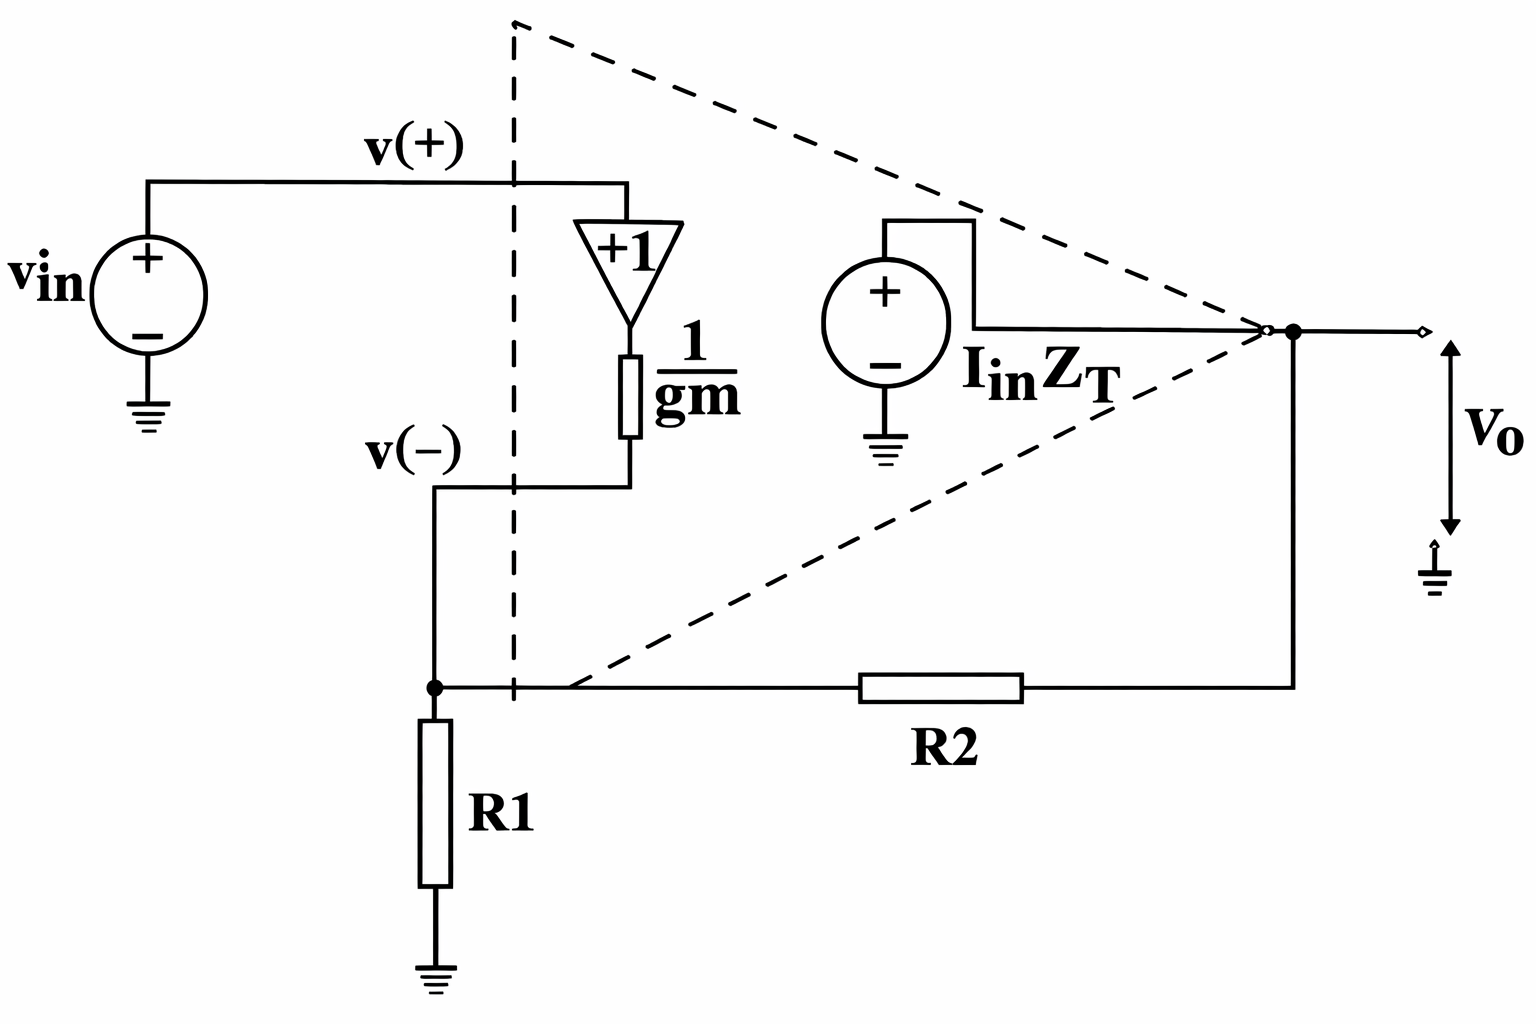
\includegraphics[width=0.5\linewidth]{Imagenes/3.2.png}
    \caption{}
    \label{fig:3.2}
\end{figure}
La apertura del lazo de la (\ref{fig:3.3}) prepara convenientemente al amplificador para efectuar el análisis 
propuesto utilizando la expresión de Black. 
\begin{figure}[H]
    \centering
    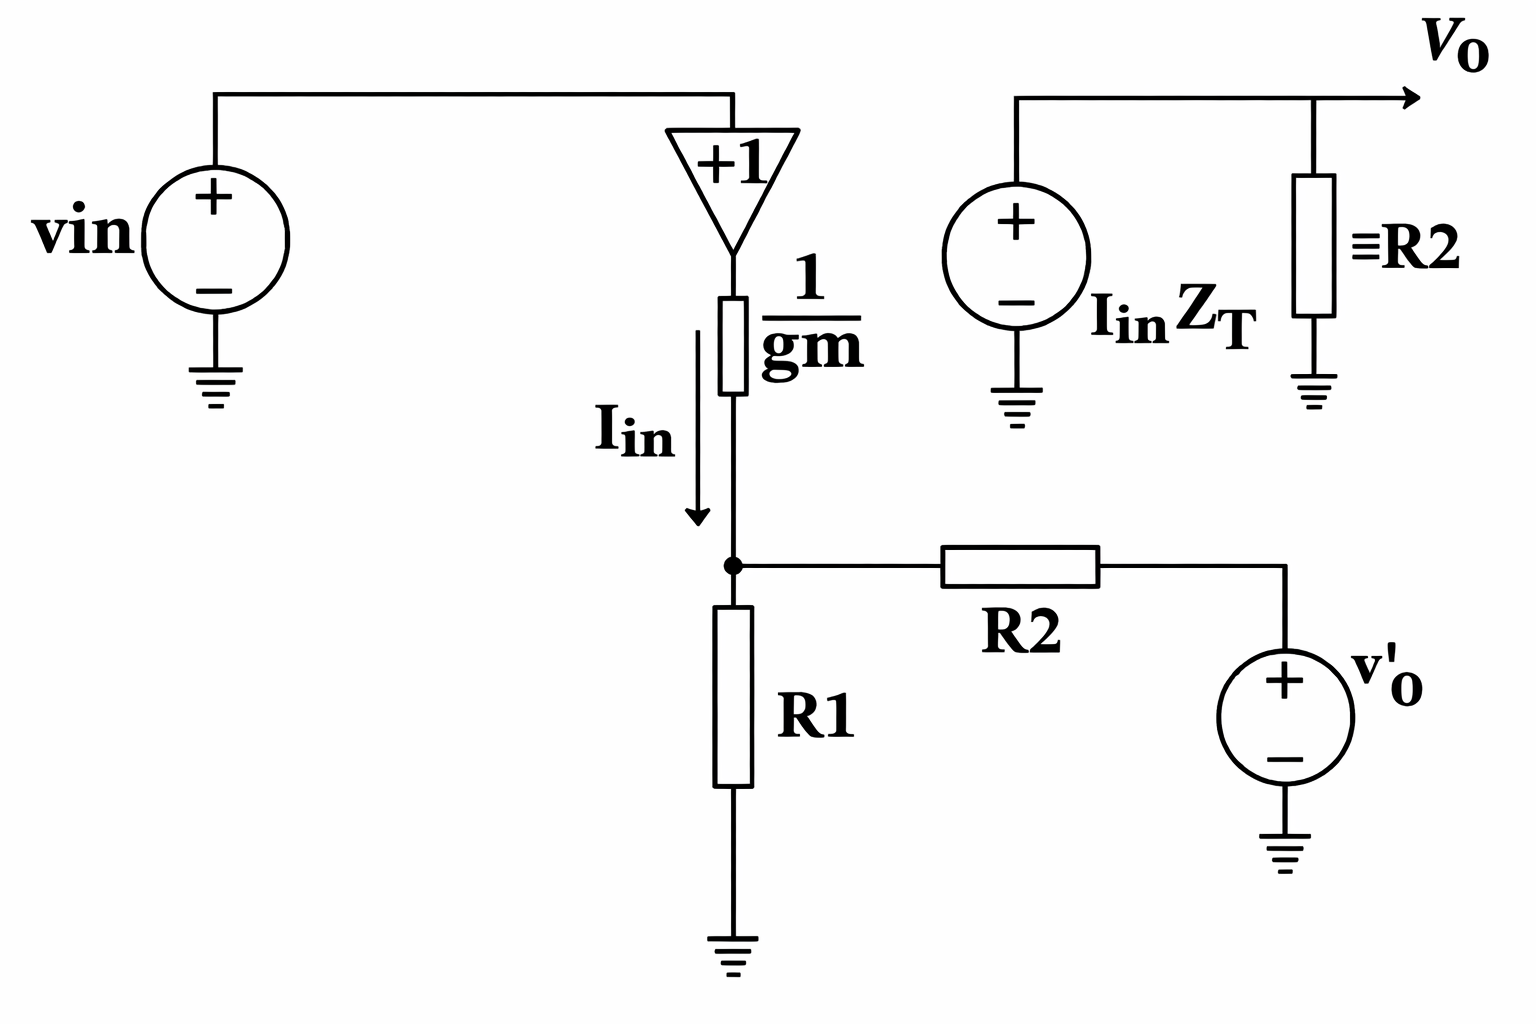
\includegraphics[width=0.5\linewidth]{Imagenes/3.3.png}
    \caption{}
    \label{fig:3.3}
\end{figure}
Considerar ideal el buffer de entrada implica que
$Z_{in+} = \infty$; $Z_{in-} = 0$ y $V_+ = V_-$.

Luego la ganancia de lazo abierto evaluada arroja el siguiente resultado:

\begin{equation}
GLA = \frac{V_o}{V'_{in}} = \frac{I_{in} Z_t}{I_{in} (R_1 \parallel R_2)} = \frac{Z_t}{R_1 \parallel R_2}
\label{eq:3.2}
\end{equation}
De igual manera la ganancia de lazo resulta:

\begin{equation}
GL|_{v'_{in}=0} = \left( \frac{v_0}{v'} \right) = - \frac{Z_t}{R_2}
\label{eq:3.3}
\end{equation}

Finalmente la ganancia de lazo cerrado es

\begin{equation}
A_{vf} = \left( \frac{v_0}{v_{IN}} \right) == \frac{\frac{Z_t}{R_p}}{1 + \frac{Z_t}{R_2}} = \frac{R_2 / R_p}{1 + \frac{1}{Z_t / R_2}} = \frac{\overbrace{1 + R_2 / R_1}^{Avfi}}{1 - \frac{1}{T}}
\label{eq:3.4}
\end{equation}

La expresión final de ecuación anterior, muestra la forma clásica de la ganancia no inversora del amplificador realimentado con función de transferencia de un solo polo, en términos de su valor idealizado, con el término de error producido por la ganancia de lazo finita.

$$
\varepsilon = \frac{1}{T(s)}
$$

La expresión (\ref{eq:3.2}), pone en evidencia el efecto de la baja impedancia de la entrada inversora ya que debido a esto, es inevitable que la red de realimentación cargue a la misma, haciendo que la ganancia de lazo abierto dependa inversamente de $R_p$ de la misma manera que la ganancia de lazo cerrado ($R_2/R_p$).. Esto muestra la diferencia operativa básica que tiene la CFA respecto del operacional clásico donde GLA es prácticamente invariante con la cantidad de realimentación introducida, debido a que ambas entradas son de alta impedancia

Otra diferencia relevante a remarcar, se refiere al comportamiento dinámico del CFA, que se pone en evidencia desarrollando el denominador (\ref{eq:3.4}), según se muestra a continuación

\begin{equation}
1 + \frac{1}{\frac{Z_t}{R2}} = 1 + \frac{R_2}{R_t} + sC_t R_2 \cong 1 + sC_t R_2
\label{eq:3.5}
\end{equation}

En la anterior es $R_2/Rt << 1$, debido a que por razones de optimización del comportamiento dinámico, $R_2$ debe ser del orden de $1 \text{ k}\Omega$.
Finalmente GLC puede expresarse como

\begin{equation}
Avf_{(s)} = \frac{R_2 / R_p}{1 + sC_t R_2} = \frac{Avfi}{1 + s/ \omega_H}
\label{eq:3.6}
\end{equation}

\begin{equation}
\omega_H = 1/CtR2
\label{eq:3.7}
\end{equation}

El análisis realizado permite extraer conclusiones relevantes respecto del comportamiento dinámico del CFA. Por ejemplo, si se varia la ganancia de señal $R_2/R_p=1+R_2/R_1$ , a través de $R_1$ y manteniendo constante $R_2$, tanto el ancho de banda como la ganancia del lazo, $T(s)$, permanecen constantes, mientras que la ganancia de lazo abierto varia en el mismo sentido y magnitud que la de señal. Una consecuencia de esto es que tenga característica producto Ganancia- Ancho de Banda, creciente con la ganancia pudiendo llegar al GHz.
La (\ref{fig:3.4}) muestra en diagrama de Bode, las magnitudes de las ecuaciones desarrolladas, dando una 
clara visión del comportamiento del dispositivo para dos diferentes ganancias de lazo cerrado. 
\begin{figure}[H]
    \centering
    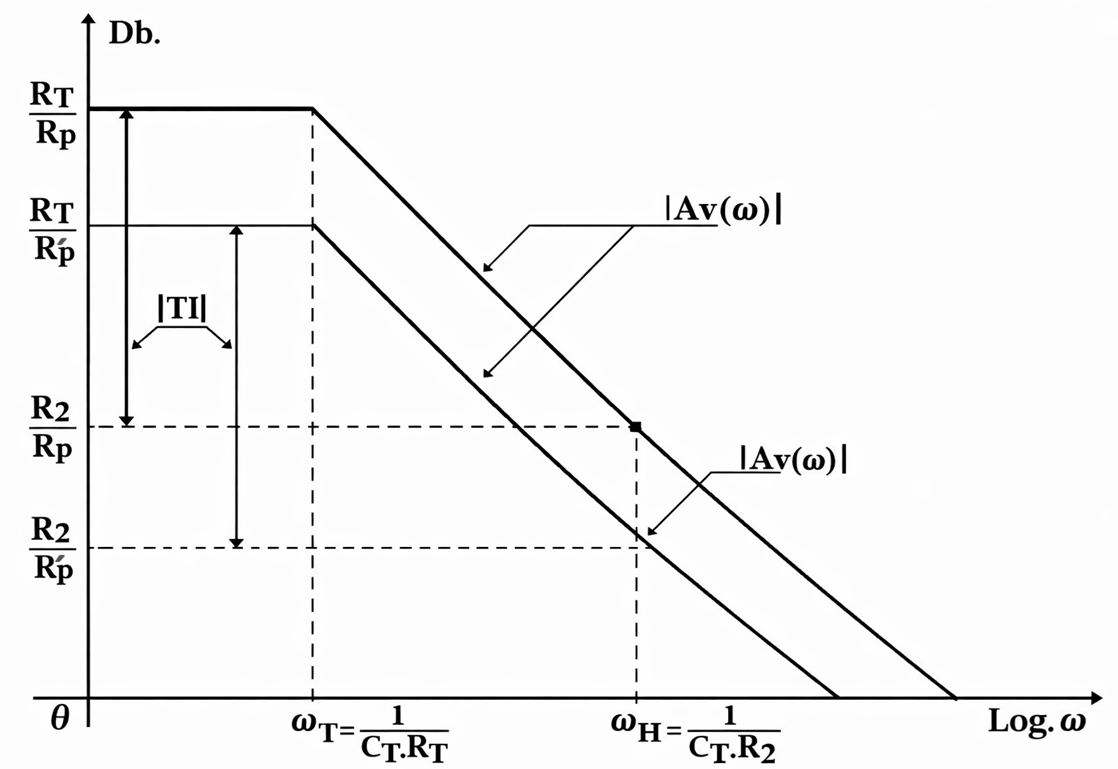
\includegraphics[width=0.5\linewidth]{Imagenes/3.4.png}
    \caption{}
    \label{fig:3.4}
\end{figure}
Las conclusiones obtenidas se pueden extender a otras configuraciones amplificadoras, así por ejemplo la respuesta de una configuración inversora se deduce de fig \ref{fig:3.3}, excitando con el generador de señal el extremo de R1, del que se obtienen las siguientes relaciones.

\begin{equation}
GLA|_{V'=0} = \left( \frac{v_0}{I_{in}} \right) \left( \frac{I_{IN}}{V_{in}} \right) = Z_t . \left( - \frac{1}{R_1} \right) = - \frac{Z_t}{R_1}
\label{eq:3.8}
\end{equation}

La ganancia de lazo, independiente del punto de inyección de señal, responde a la expresión deducida en (\ref{eq:3.3}).

Finalmente se obtiene para la ganancia de lazo cerrado la siguiente ecuación

\begin{equation}
A_{vf} = \left( \frac{v_0}{V_{in}} \right) = \frac{- \frac{Z_t}{R_1}}{1 + \frac{Z_t}{R_2}} = \frac{- R_2 / R_1}{1 + \frac{1}{Z_t / R_2}} = \frac{\overbrace{- R_2 / R_1}^{Avfi}}{1 - \frac{1}{T}}
\label{eq:3.9}
\end{equation}

Utilizando el desarrollo del denominador de la expresión dada en (\ref{eq:3.6}), la anterior se expresa:

El procedimiento de diseño del amplificador comienza con la selección de la resistencia de realimentación ($R_2$), para fijar el ancho de banda y cuyo valor tiene un mínimo dado por razones de estabilidad, tema que será analizado en detalle en secciones posteriores. No obstante en la hoja de datos del dispositivo se recomienda un valor, (En torno al $\text{k}\Omega$), que optimiza en términos de estabilidad su operación dinámica. Debido a esto para implementar un amplificador separador (Buffer), a diferencia del caso VFA, se debe hacer, $R_1= \infty$ y $R_2 \neq 0$, por las razones arriba comentadas.
La resistencia $R_1$, es fijada por requerimiento de ganancia de lazo cerrado, obviamente el incremento de esta implica disminución de la primera de modo que para ganancias elevadas el valor de $R_1$ es comparable con la impedancia de entrada no inversora ($R_{IN} = 1/gm \approx 30 \text{ Ohms}$) que fue supuesta nula en el análisis precedente pero dejaría de serlo en la situación planteada. Las expresiones encontradas en las configuraciones analizadas se pueden modificar teniendo en cuenta este efecto. Por ejemplo para la no inversora se obtiene de figura 3.3

\begin{equation}
GLA|_{v'=0} = \left( \frac{v_0}{v_{in}} \right) = \frac{Z_t}{R_{IN} + R_p}
\label{eq:3.10}
\end{equation}

La anterior se puede expresar de manera diferente multiplicado y dividiendo por la ganancia de lazo cerrado no inversora ideal ($(Avfi)_N$) y desarrollando el denominador resultante.

$$
GLA|_{v'=0} = \left( \frac{v_0}{v_{IN}} \right) = \frac{Z_t \overbrace{(1 + R_2 / R_1)}^{(Avfi)_{NI}}}{(R_{IN} + R_p)(1 + R_2 / R_1)} = \frac{Z_t (A_{vfi})_{NI}}{R_2 + R_{IN} (A_{vfi})_{NI}}
$$

La ganancia de lazo ($T$) resulta

\begin{equation}
GL|_{vin'=0} = \left( \frac{v_0}{v'} \right) = - \left( \frac{Z_t}{R_2 + (R_{IN} // R_1)} \right) \left( \frac{R_1}{R_{IN} + R_1} \right) = - \frac{Z_t}{R_2 + R_{IN} (A_{vfi})_{NI}}
\label{eq:3.11}
\end{equation}

Finalmente la ganancia de lazo cerrado es

\begin{equation}
GLC = \left( \frac{v_0}{v_{IN}} \right) = \frac{(A_{vfi})_{NI}}{1 + \frac{R_2 + R_{IN}(A_{vfi})_{NI}}{Z_t}} = \frac{(A_{vfi})_{NI}}{1 - \frac{1}{T}}
\label{eq:3.12}
\end{equation}

Repitiendo el análisis para la configuración inversora de obtiene

$$
GLA|_{V'=0} = \left( \frac{v_0}{v_{in}} \right) = - \frac{Z_t}{(R_1 + (R_{IN} // R_1)).(\frac{R_{IN} + R_2}{R_2})}
$$

La anterior luego de un tratamiento algebraico semejante al realizado en (3.11) se expresa según la siguiente.

\begin{equation}
GLA|_{V'=0} = \left( \frac{v_0}{v_{in}} \right) = \frac{Z_t (A_{vfi})_{In}}{R_2 + R_{IN} (A_{vfi})_{NI}}
\label{eq:3.13}
\end{equation}

Relacionando la anterior con la ganancia de lazo (3.11), se obtiene

\begin{equation}
GLC = \left( \frac{v_0}{v_{in}} \right) = \frac{(A_{vfi})_{In}}{1 + (\frac{R_2 + R_{IN}(A_{vfi})_{NI}}{Z_t})} = \frac{(A_{vfi})_I}{1 - \frac{1}{T}}
\label{eq:3.14}
\end{equation}
\subsection{Errores}
En general este amplificador tiene especificaciones de fuentes de errores en continua más pobres que el VFA y no obstante el análisis de sus efectos es similar al caso anterior, el tratamiento referente a las corrientes de polarización es diferente debido a la asimetría estructural de las entradas no inversora e inversora. Por esto es que la técnica de ecualización de las impedancias vistas desde ambas entradas utilizadas para minimizar el error de corrientes de polarización en el A.O, no sea aplicable al CFA, tal es así que no se publica el offset de corriente, ($I_{OS}$). Es aconsejable analizar las especificaciones de la hoja de datos antes de tomar alguna medida correctiva.

El offset de tensión es elevado, (Ej. $5\text{mV}$) y es generalmente el error que domina en baja frecuencia

\begin{equation}
\Delta v_0 = \pm V_{os} . (A_{vfi})_{NI}
\label{eq:3.17}
\end{equation}

La evaluación de los errores producidos por la ganancia de lazo abierto no ideal, (transimpedancia finita), tiene un tratamiento similar al caso VFA, ya que tanto el de continua como los dinámicos se derivan de la misma expresión general, (Ej. Ecuación. 3.4 y 3.14).
\newpage
\section{Amplificadores de transconductancia (OTA)}
\subsection*{Introducción}
Los amplificadores de transconductancia integrados se comportan como fuentes de corriente controladas por tensión, siendo obviamente el parámetro de transferencia, la transconductancia ($g_m$). Desde este punto de vista emulan el comportamiento de los transistores discretos, mostrando modelos lineales equivalentes semejantes aunque con mucho más refinamiento en la precisión y control de sus parámetros.

Existen dos tipos bien diferenciados según se deriven de la arquitectura de amplificadores VFA o CFA, no obstante ambos estructuralmente tienen solo dos etapas, una primera diferencial cuya corriente es reproducida a la salida por la segunda, que se corresponde con un espejo de corriente. A diferencia de los dos tipos de amplificadores estudiados previamente estos pueden operar linealmente sin realimentación (Amplificación Directa), teniendo en esta modalidad excelente performance en altas frecuencias debido al reducido número de etapas que poseen.
\subsection{OTA-VFA}
Este tipo utiliza la etapa de entrada del diferencial clásico de los VFA, con versiones comerciales de tecnología Bipolar o MOS, en consecuencia presentan muy alta impedancia en los dos terminales de entrada y alta en el de salida. La figura \ref{fig:4.1}, muestra el símbolo frecuentemente utilizado y el modelo lineal equivalente en bajas frecuencias.
\begin{figure}[H]
    \centering
    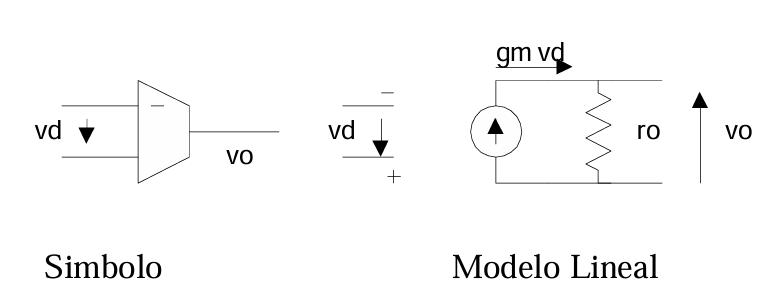
\includegraphics[width=0.5\linewidth]{Imagenes/4.1.png}
    \caption{}
    \label{fig:4.1}
\end{figure}
La transconductancia ($g_m$) del conjunto se corresponde con la del diferencial de entrada y es función directa de la corriente de polarización del mismo que puede ser variada externamente por tensión dentro de los límites especificados en la hoja de datos respectiva.

\begin{equation}
g_m = \frac{I_0}{2 V_t}
\label{eq:4.1}
\end{equation}

$I_0 = \text{Corriente de polarización}$

El modo diferencial máximo depende del grado de distorsión admitida, para una etapa diferencial bipolar simple no supera los $2V_t$ ($\cong \pm 50\,\text{mV}$ a $25\,^\circ\text{C}$), este rango puede ser ampliado al orden del voltio, con el agregado de diodos de linealización a la entrada, que además compensan térmicamente la transconductancia cuando los diodos están integrados al chip. En la actualidad la mayoría de las versiones comerciales los tienen incorporado.
\subsubsection{Aplicaciones}
La posibilidad de ajuste externo del parámetro de transferencia $g_m$ mediante la corriente de polarización, hace que este tipo de amplificadores encuentren amplio campo de aplicación, en la realización de circuitos eléctricamente sintonizables, tales como amplificadores de ganancia controlada, osciladores y filtros activos. A continuación se analizarán algunas de las aplicaciones típicas comentadas.

\textbf{Amplificador Directo}

El OTA puede ser utilizado como amplificador de tensión directo o en configuraciones realimentadas. En el primer caso Fig \ref{fig:4.2}, la ganancia de tensión puede ser ajustada externamente a través de la transconductancia $g_m$ (\ref{eq:4.2})

\begin{equation}
A_v = g_m . Z_L
\label{eq:4.2}
\end{equation}

\begin{figure}[H]
    \centering
    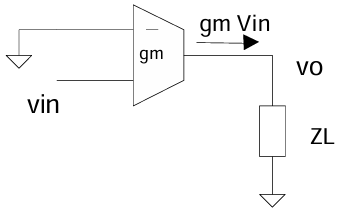
\includegraphics[width=0.5\linewidth]{Imagenes/4.2.png}
    \caption{Amplificador directo de ganancia controlada}
    \label{fig:4.2}
\end{figure}
\subsubsection{Configuraciones realimentadas}
Las configuraciones realimentadas negativamente son muy utilizadas para simular componentes pasivos, tales como resistores e inductores eléctricamente sintonizables. Por ejemplo la configuración de figura \ref{fig:4.3} se comporta en bajas frecuencias como una resistencia con un extremo a tierra, de valor inverso a la transconductancia del OTA ($r_m=1/g_m$).

En efecto asumiendo el modelo de fig \ref{fig:4.1}, en términos idealizados ($r_i = r_o = \infty$), se deduce por simple inspección la siguiente relación para la impedancia de entrada.

\begin{equation}
Z_{in} = \frac{V_{in}}{I_{in}} = \frac{V_{in}}{g_m V_{in}} = \frac{1}{g_m} = r_m
\label{eq:4.3}
\end{equation}
\begin{figure}[H]
    \centering
    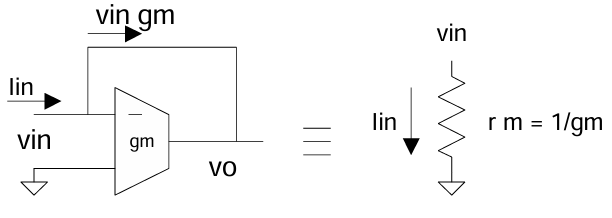
\includegraphics[width=0.85\linewidth]{Imagenes/4.3.png}
    \caption{Resistencia a tierra}
    \label{fig:4.3}
\end{figure}
\subsection*{Ejemplo 4.1}
\noindent\rule{\textwidth}{0.4pt}

\vspace{0.2cm}
\noindent Analizar el efecto de la impedancia de salida finita, sobre el valor idealizado, dado por (\ref{eq:4.3}).
\vspace{0.2cm}

\noindent\rule{\textwidth}{0.4pt}

\vspace{0.2cm}
\noindent Para el análisis propuesto se utilizará la fórmula de Blackman, con el circuito modelado como lo muestra la figura \ref{fig:4.4}, de la que se deducen las GL respectivas ($T_{cc}$ y $T_{ca}$).
\begin{figure}[H]
    \centering
    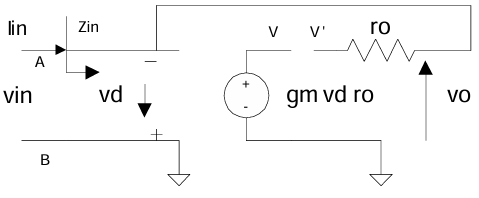
\includegraphics[width=0.65\linewidth]{Imagenes/4.4.png}
    \caption{Impedancia del sistema muerto}
    \label{fig:4.4}
\end{figure}
$$
Z_{in}|_{V'=0} = \frac{V_{in}}{I_{in}} = r_O
$$

Es fácil ver que la ganancia de lazo para la sección de interés (A-B), en cortocircuito es nula debido a que:

$$
v_d = 0 \Rightarrow v = 0 \hspace{3cm} T_{cc} = \left( \frac{v}{v'} \right) \bigg|_{vin=0} = 0
$$

En cambio para la sección abierta es $v_d = v'$, luego:

$$
T_{ca} = \left( \frac{v}{v'} \right) \bigg|_{Iin=0} = -g_m \cdot r_O
$$

Finalmente

$$
Z_{if} = \frac{r_O}{(1+g_m \cdot r_O)}
$$

En la anterior se ve que si $r_O \to \infty \Rightarrow Z_{in} \to 1/g_m$
La configuración un tanto más compleja de fig \ref{fig:4.5}, logra simular un resistor flotante, cargando entrada y salida del OTA ($O_1$), con resistencias a tierra iguales, simuladas por ($O_2$) y ($O_3$), respectivamente.

En efecto en el nudo de entrada se cumple

\begin{equation}
I_{in} = -(V_O - V_{in}) \cdot g_m \rightarrow \frac{(V_{in} - V_O)}{I_{in}} = \frac{1}{g_m} = r_m
\label{eq:4.4}
\end{equation}

Tomando el circuito como un súper nodo se deduce la impedancia vista desde el nodo $V_O$.

\begin{equation}
I_{in} = -I_O \Rightarrow \frac{(V_O - V_{in})}{I_O} = \frac{1}{g_m} = r_m
\label{eq:4.5}
\end{equation}

\begin{figure}[H]
    \centering
    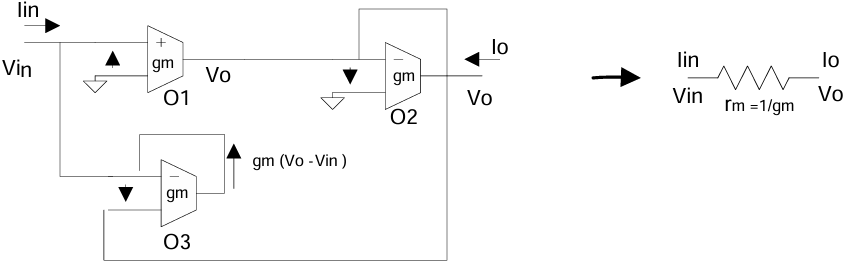
\includegraphics[width=0.65\linewidth]{Imagenes/4.5.png}
    \caption{Resistor flotante}
    \label{fig:placeholder}
\end{figure}

El circuito anterior cargado con un capacitor, genera una sección de filtro pasabajos de primer orden, cuya frecuencia de corte puede ajustarse eléctricamente a través de $g_m$.
\begin{figure}[H]
    \centering
    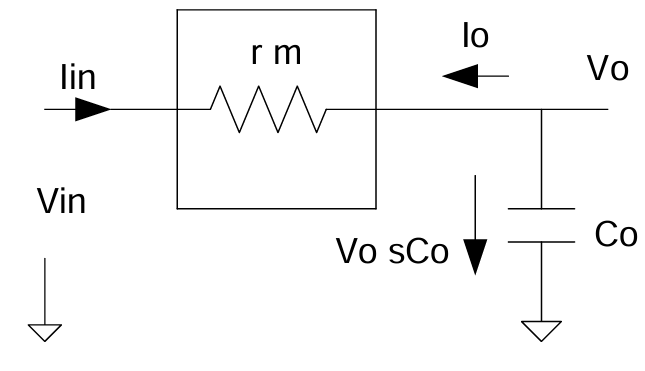
\includegraphics[width=0.5\linewidth]{Imagenes/4.6.png}
    \caption{Sección pasabajos R-C}
    \label{fig:placeholder}
\end{figure}
En efecto a partir de figura \ref{fig:4.6}, donde el bloque $r_m$ representa al circuito de figura \ref{fig:4.5}, se deduce la siguiente función de transferencia.
\begin{equation}
I_O = \frac{(V_O - V_{in})}{r_m} = -V_O \cdot s \cdot C \quad \rightarrow \quad A_v(s) = \frac{V_O}{V_{in}} = \frac{1}{(1 + s \cdot C \cdot r_m)}
\label{eq:4.6}
\end{equation}

Se denominan \textit{giradores} a aquellos circuitos que muestran una impedancia de entrada que es la inversa de la de carga. Esta transformación permite simular inductores, cargando un girador con un capacitor. La conexión OTA de figura \ref{fig:4.7} es un ejemplo y de ella se deducen las siguientes relaciones.

\begin{figure}[H]
    \centering
    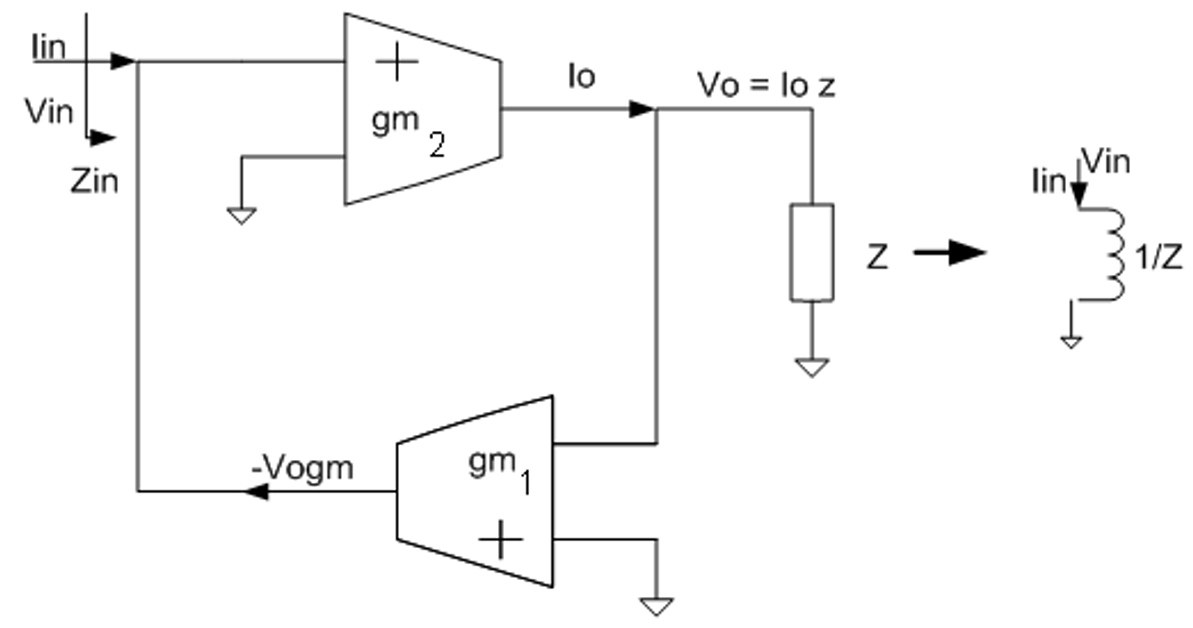
\includegraphics[width=0.5\linewidth]{Imagenes/4.7.png}
    \caption{Girador(inductor a tierra)}
    \label{fig:placeholder}
\end{figure}
\begin{equation}
I_{in} = V_O \cdot g_{m1} = V_{in} \cdot g_{m1} \cdot Z \cdot g_{m2} \quad \Rightarrow \quad \frac{V_{in}}{I_{in}} = \frac{1}{g_{m1} \cdot g_{m2} \cdot Z}
\label{eq:4.6}
\end{equation}

Si $Z = \frac{1}{s \cdot Cx} \Rightarrow Z_{in} = s \cdot \left( \frac{Cx}{g_{m1} \cdot g_{m2}} \right) = s \cdot Lx \quad \text{donde:} \quad Lx = \left( \frac{Cx}{g_{m1} \cdot g_{m2}} \right)$
\begin{equation}
\label{eq:4.7}
\end{equation}

La conexión de dos giradores similares al de figura \ref{fig:4.7} excitando en contrafase la impedancia $Z$ (Fig \ref{fig:4.8}), simulan un inductor flotante conectado entre entrada y salida, cuando aquella es un capacitor.

$$
Vx = (V_O \cdot g_{m1} - V_{in} \cdot g_{m1}) \cdot Z
$$

Si $Z = \frac{1}{s \cdot Cx}$ e $I_{in} = -Vx \cdot g_{m2} \Rightarrow Z_{in} = \left( \frac{V_{in} - V_O}{I_{in}} \right) = \left( \frac{s \cdot Cx}{g_{m1} \cdot g_{m2}} \right)$
\begin{equation}
\label{eq:4.8}
\end{equation}

De igual manera la impedancia vista desde el otro extremo será:

$$
I_{in} = -I_O \quad \Rightarrow \quad Z_0 = \left( \frac{V_O - V_{in}}{I_0} \right) = s \cdot Lx
$$
\begin{figure}[H]
    \centering
    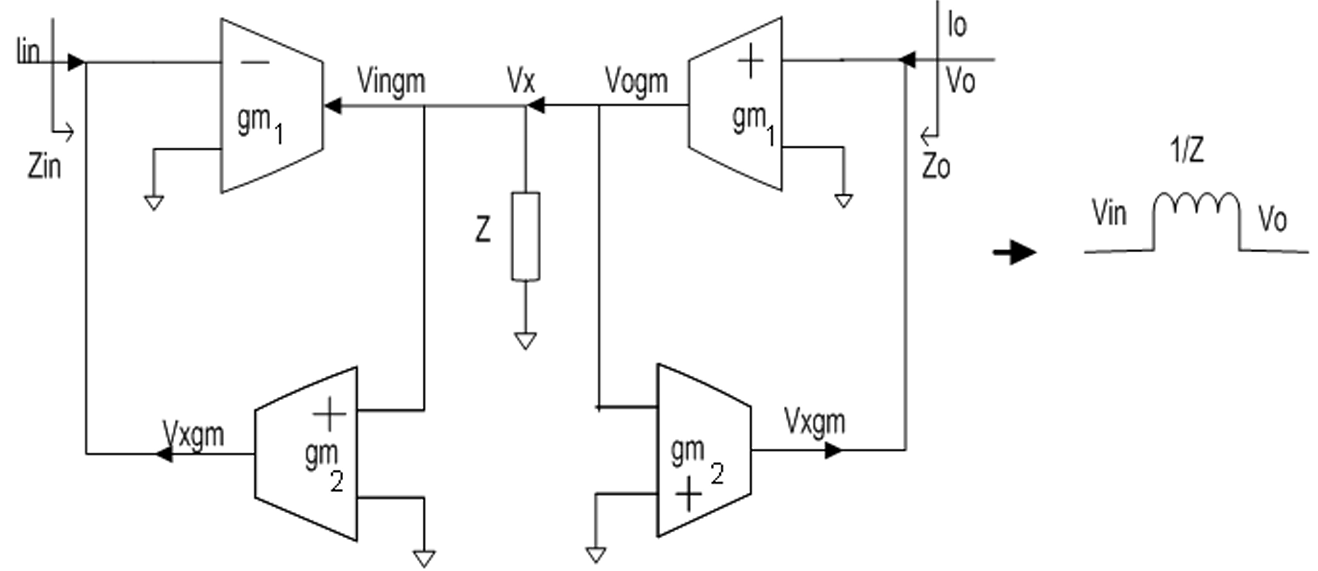
\includegraphics[width=0.65\linewidth]{Imagenes/4.8.png}
    \caption{Inductor flotante}
    \label{fig:4.8}
\end{figure}
Cargando la salida del inductor flotante de figura \ref{fig:4.8}, con un capacitor, se genera una sección pasabajos de segundo orden no disipativa ($L-C$).

En efecto en referencia a la figura \ref{fig:4.9} y a partir de la ecuación (\ref{eq:4.8}), se deduce la función de transferencia respectiva.

\begin{equation}
\text{Siendo: } I_0 = -V_0 \cdot s \cdot C_0 = \frac{(V_0 - V_{in})}{s \cdot Lx} \quad \Rightarrow \quad \frac{V_0}{V_{in}} = \frac{1}{Lx \cdot C_0} \cdot \frac{1}{\left( s^2 + \frac{1}{Lx \cdot C_0} \right)}
\end{equation}

\begin{figure}[H]
    \centering
    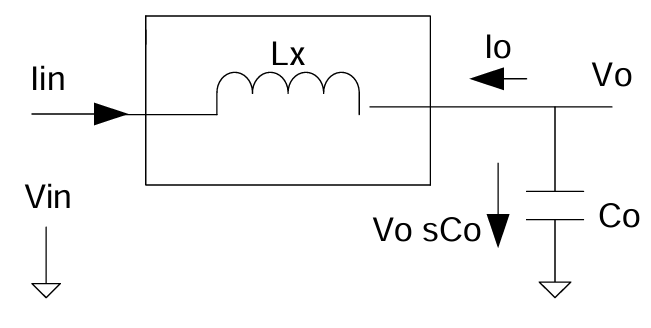
\includegraphics[width=0.5\linewidth]{Imagenes/4.9.png}
    \caption{Sección pasabajos L-C}
    \label{fig:4.9}
\end{figure}
Las versiones comerciales de estos integrados incluyen en el mismo chip un Buffer que permite ampliar el campo de aplicaciones posibles. Por ejemplo se puede configurar un amplificador operacional clásico, por la conexión en cascada de ambos (fig \ref{fig:4.10}). Obviamente la elevada impedancia de entrada del buffer ($Z_{inb}$), mueve en el mismo sentido la ganancia de tensión del conjunto ($A_v = g_m \cdot Z_{inb}$), obligando a que sus aplicaciones se limiten a configuraciones realimentadas.

\begin{figure}[H]
    \centering
    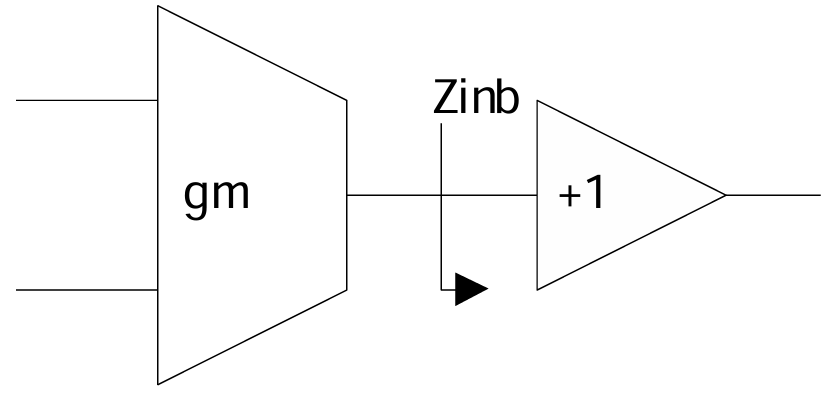
\includegraphics[width=0.5\linewidth]{Imagenes/4.10.png}
    \caption{}
    \label{fig:4.10}
\end{figure}

\subsection{OTA-CFA (transistor diamante)}
Esta segunda versión de amplificadores OTAs, denominada por sus diseñadores (Burr-Brown Corp), como Fuente de Corriente Diamante (DCS) o también Transistor Diamante (DT) se deriva de la arquitectura bipolar CFA y utiliza la misma etapa diferencial de entrada (Buffer Diamante), en consecuencia la impedancia de entrada del terminal no inversor, denominada Base del transistor Diamante, es muy elevada y en cambio la del inversor (Emisor del TD) muy baja. Ambos emulan una junta cuya relación corriente de emisor-tensión de control resulta lineal y bidireccional (Fig. \ref{fig:4.11}). El rango de modo diferencial máximo admitido con mínima distorsión se corresponde no obstante con el diferencial clásico, es decir aproximadamente $\pm 50\,\text{mV}$.
\begin{figure}[H]
    \centering
    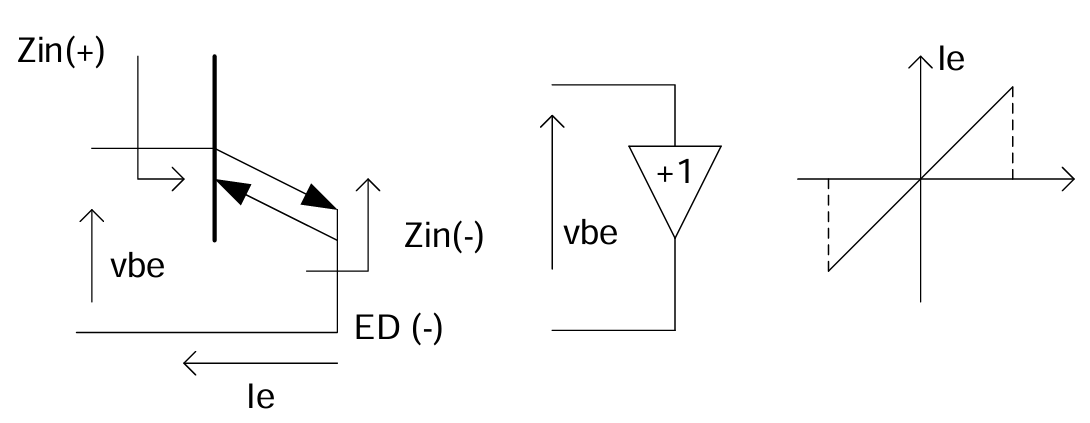
\includegraphics[width=0.5\linewidth]{Imagenes/4.11.png}
    \caption{}
    \label{fig:4.11}
\end{figure}
La etapa de salida vuelve a ser un espejo de corriente que en este caso copia con relación 1/1, la corriente del emisor cuya salida configura el colector equivalente ($C_d$), con una impedancia asociada del mismo orden de magnitud que el caso clásico.

La fig. \ref{fig:4.12}a, muestra el símbolo frecuentemente utilizado para representarlo, la doble flecha recuerda su característica bidireccional en términos de corriente total en sus terminales, y en fig \ref{fig:4.12}b el modelo en baja frecuencia. En virtud de que la corriente de colector reproduce en módulo y sentido la de emisor, la característica de transferencia de la fig. \ref{fig:4.11} se extiende a la corriente de colector.
\begin{figure}[H]
    \centering
    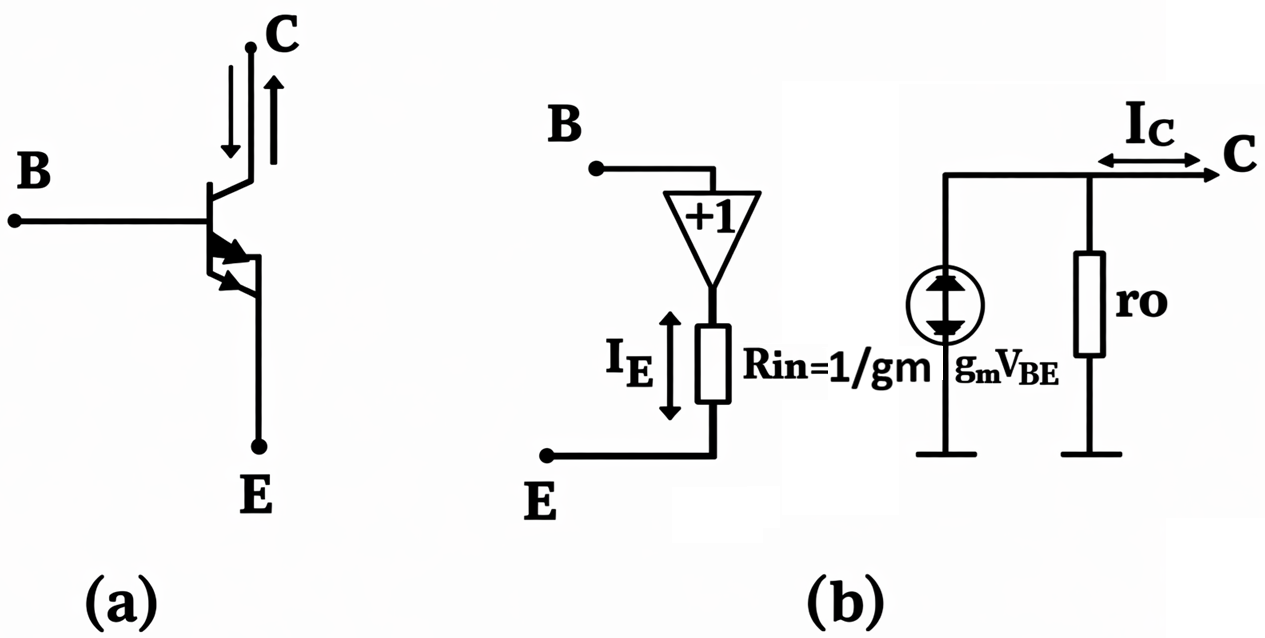
\includegraphics[width=0.5\linewidth]{Imagenes/4.12.png}
    \caption{}
    \label{fig:4.12}
\end{figure}
La fig. \ref{fig:4.13}, extiende y cuantifica los conceptos desarrollados mostrando un cuadro de características y parámetros comparativo con los dos elementos discretos de juntura, (JFET y BJT), que operan como fuentes de corriente controlada.
\begin{figure}[H]
    \centering
    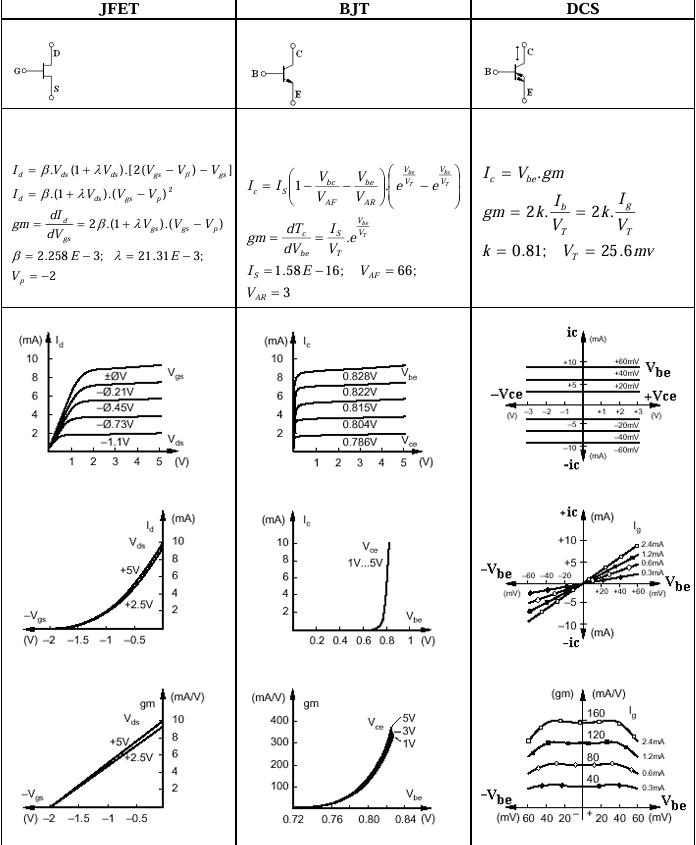
\includegraphics[width=1\linewidth]{Imagenes/4.13.png}
    \caption{Cortesía Burr-Brown Corp.}
    \label{fig:4.13}
\end{figure}
\textbf{Amplificador directo}
De igual manera que el tipo OTA-VFA, el TD puede operar como amplificador directo de ganancia controlada. El campo de aplicación relevante de esta aplicación es en muy alta frecuencia, como excitador de cargas con fuertes componentes capacitivas (Line Driver). En los párrafos siguientes se analiza de un modo general, su modo de operación en bajas frecuencias poniendo en evidencia sus características amplificadoras en cuatro cuadrantes, como lo muestra la fig \ref{fig:4.14}b, donde la ecuación de la recta de carga derivada de \ref{fig:4.14}a será para $R_{in}=1/g_m \ll R_e$:

\begin{equation}
v_{ce} = v_c - v_e =  i_c (R_c - R_e)
\label{eq:4.9}
\end{equation}
\begin{figure}[H]
    \centering
    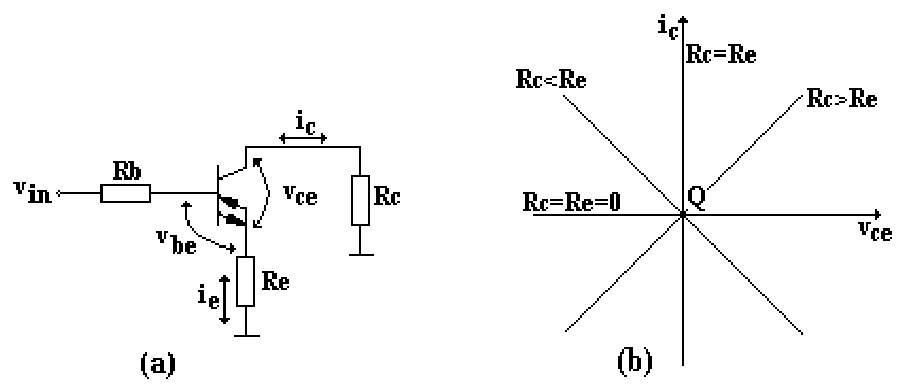
\includegraphics[width=0.75\linewidth]{Imagenes/4.14.png}
    \caption{}
    \label{fig:4.14}
\end{figure}

Luego, según muestra la fig. \ref{fig:4.14}b la pendiente de la recta de carga será positiva, negativa, infinita o nula, según sean los valores relativos de $R_c$ y $R_e$. El punto de operación en reposo ($Q$), coincidirá con el origen de coordenadas.

Si en cambio la señal $V_{in}$ tuviere componente de continua (la que no debe superar el rango de modo diferencial admitido), puede ocurrir cualquiera de las situaciones mostradas en la fig. \ref{fig:4.15}, según sea la polaridad de aquella y los valores relativos de las resistencias ya mencionadas.
\begin{figure}[H]
    \centering
    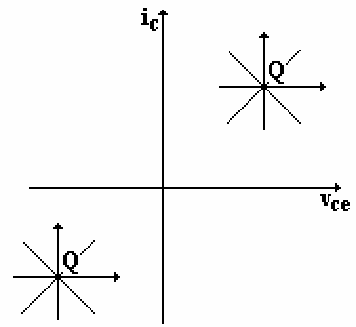
\includegraphics[width=0.5\linewidth]{Imagenes/4.15.png}
    \caption{}
    \label{fig:4.15}
\end{figure}
En general, las configuraciones simples o compuestas realizadas con transistores discretos clásicos, pueden también ser emuladas por el Transistor Diamante, más algunas que le son propias. No obstante siempre pueden ser analizadas por simple inspección.
\textbf{Emisor común}
Este modo de operación se corresponde con el esquema de la fig. \ref{fig:4.12} y se repite en la fig. \ref{fig:4.16}. De ellos se deducen las siguientes relaciones:

$$
v_0 = i_c \cdot R_c \quad \therefore \quad i_c = i_e = \frac{V_{in}}{R_e + \frac{1}{g_m}}
$$

\begin{equation}
A_v = \frac{V_0}{V_{in}} = \frac{R_c}{R_e + \frac{1}{g_m}} = \frac{\frac{R_c}{R_e}}{1 + \frac{1}{g_m \cdot R_e}}
\tag{4.10}
\end{equation}

Si se desprecia la resistencia de entrada en emisor, se obtiene la expresión clásica de la ganancia de tensión

\begin{equation}
R_e \gg \frac{1}{g_m} \quad \Rightarrow \quad A_v = \frac{R_c}{R_e}
\tag{4.11}
\end{equation}

Se obtiene máxima ganancia de tensión haciendo $R_e=0$

\begin{equation}
A_v = g_m \cdot R_c
\tag{4.12}
\end{equation}

La fig \ref{fig:4.16}c muestra la recta de carga para este último caso.
\begin{figure}[H]
    \centering
    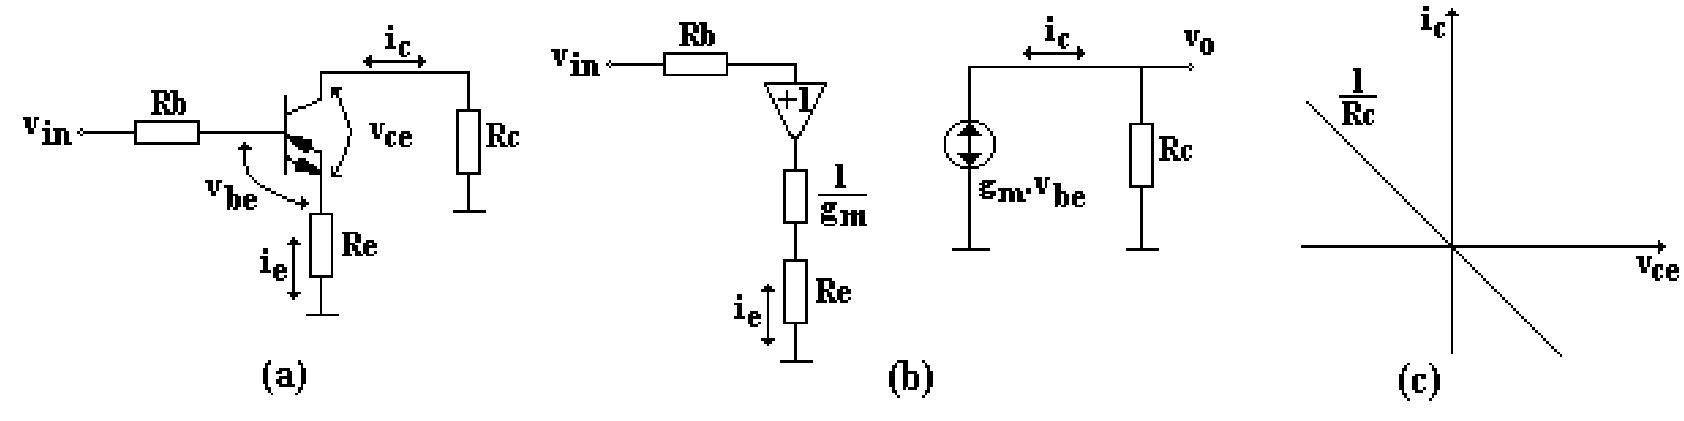
\includegraphics[width=0.95\linewidth]{Imagenes/4.16.png}
    \caption{}
    \label{fig:4.16}
\end{figure}
\textbf{Base común}
Esta configuración (fig \ref{fig:4.17}), genera las mismas funciones de transferencia que la anterior, excepto la inversión de fase entrada salida. En consecuencia la ganancia de tensión se expresa, según que la resistencia de emisor sea nula o no con alguna de las mostradas en (\ref{eq:4.13}).
\begin{figure}[H]
    \centering
    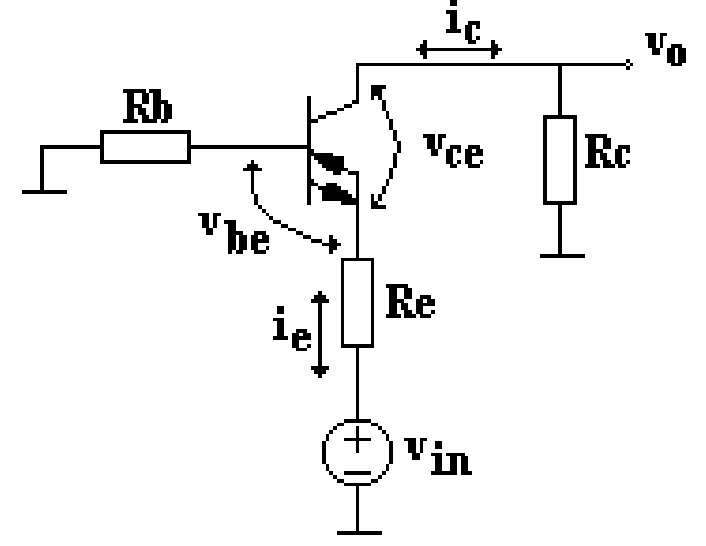
\includegraphics[width=0.5\linewidth]{Imagenes/4.17.png}
    \caption{}
    \label{fig:4.17}
\end{figure}
Esta configuración (fig \ref{fig:4.17}), genera las mismas funciones de transferencia que la anterior, excepto la inversión de fase entrada salida. En consecuencia la ganancia de tensión se expresa, según que la resistencia de emisor sea nula o no con alguna de las mostradas en (\ref{eq:4.13}).

\begin{equation}
A_v = \frac{-R_c}{R_e + \frac{1}{g_m}} \cong -\frac{R_c}{R_e}
\label{eq:4.13}
\end{equation}

$$
A_v \bigg|_{R_e=0} = -g_m \cdot R_c
$$
\textbf{Colector común (Buffer)}
El Transistor Diamante, permite configurar dos esquemas diferentes para la función buffer. El de la fig. \ref{fig:4.18}, muestra una de ellas, que se corresponde con la conexión clásica.
\begin{figure}[H]
    \centering
    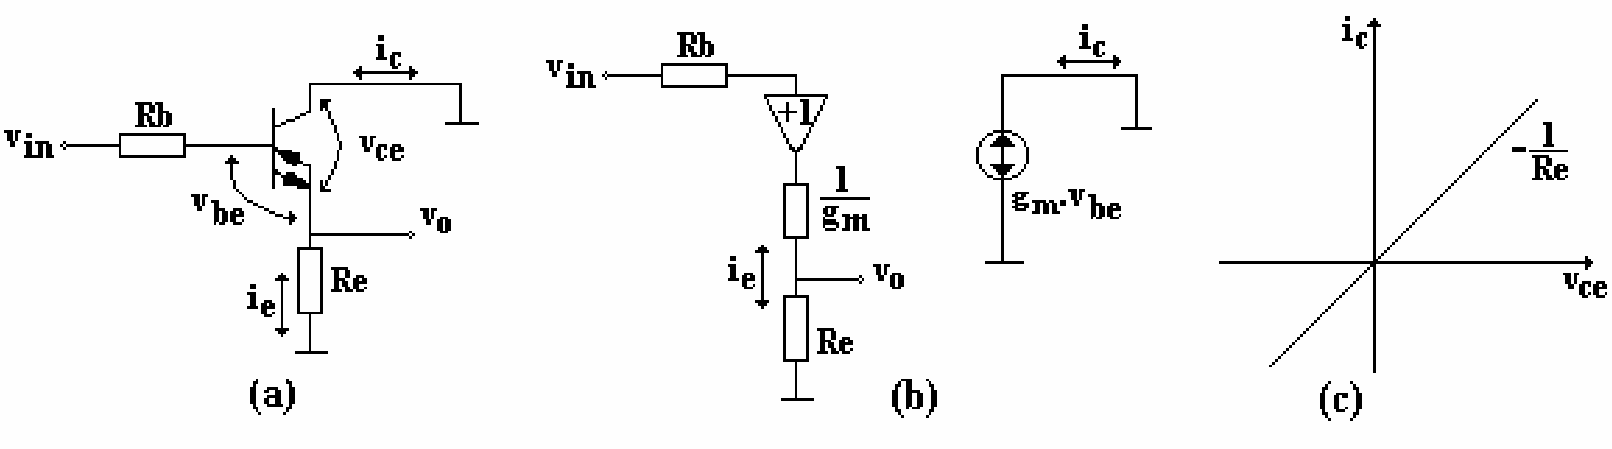
\includegraphics[width=1\linewidth]{Imagenes/4.18.png}
    \caption{}
    \label{fig:4.18}
\end{figure}
La ganancia de tensión es:

$$
v_0 = i_e \cdot R_e \quad \therefore \quad i_e = \frac{V_{in} - V_0}{\frac{1}{g_m}}
$$

\begin{equation}
A_v = \frac{V_0}{V_{in}} = \frac{1}{1 + \frac{1}{g_m \cdot R_e}} \cong 1
\tag{4.14}
\end{equation}

La fig. \ref{fig:4.19} muestra otra posibilidad de configurar un amplificador buffer duplicando la corriente en la carga. Esta conexión es propia del Transistor Diamante y mejora la función separadora del circuito anterior.
\begin{figure}[H]
    \centering
    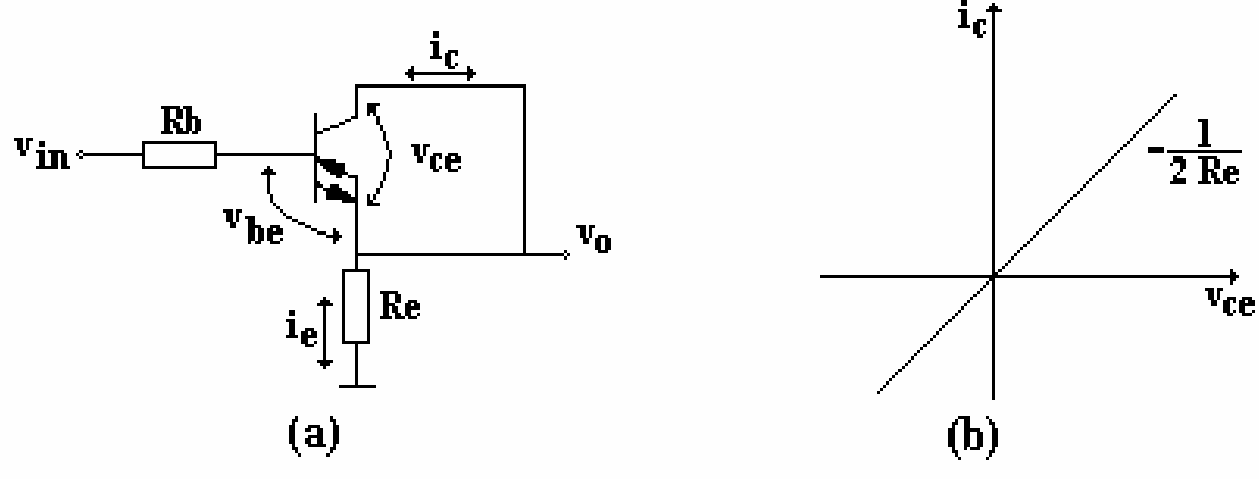
\includegraphics[width=0.75\linewidth]{Imagenes/4.19.png}
    \caption{}
    \label{fig:4.19}
\end{figure}
\begin{equation}
v_0 = 2 \cdot i_e \cdot R_e
\tag{4.15}
\end{equation}

Relacionando 4.14 y 4.15 se obtiene:

\begin{equation}
A_v = \frac{1}{1 + \frac{1}{2 \cdot R_e \cdot g_m}} \cong 1
\tag{4.16}
\end{equation}
\textbf{Configuraciones realimentadas}
La versión comercial del TD (OPA660) incluye en el mismo chip, un Buffer, que entre otras aplicaciones, permite configurar un amplificador integrado realimentado por corriente (CFA), por la conexión en cascada de ambos como muestra la figura \ref{fig:4.20}a, donde el conjunto realimentado por red exterior ($R_1$, $R_2$), configura un no inversor.

Si además se buferea la unión del divisor resistivo al emisor con un segundo Buffer (fig \ref{fig:4.20}b), resulta un amplificador operacional clásico.
\begin{figure}[H]
    \centering
    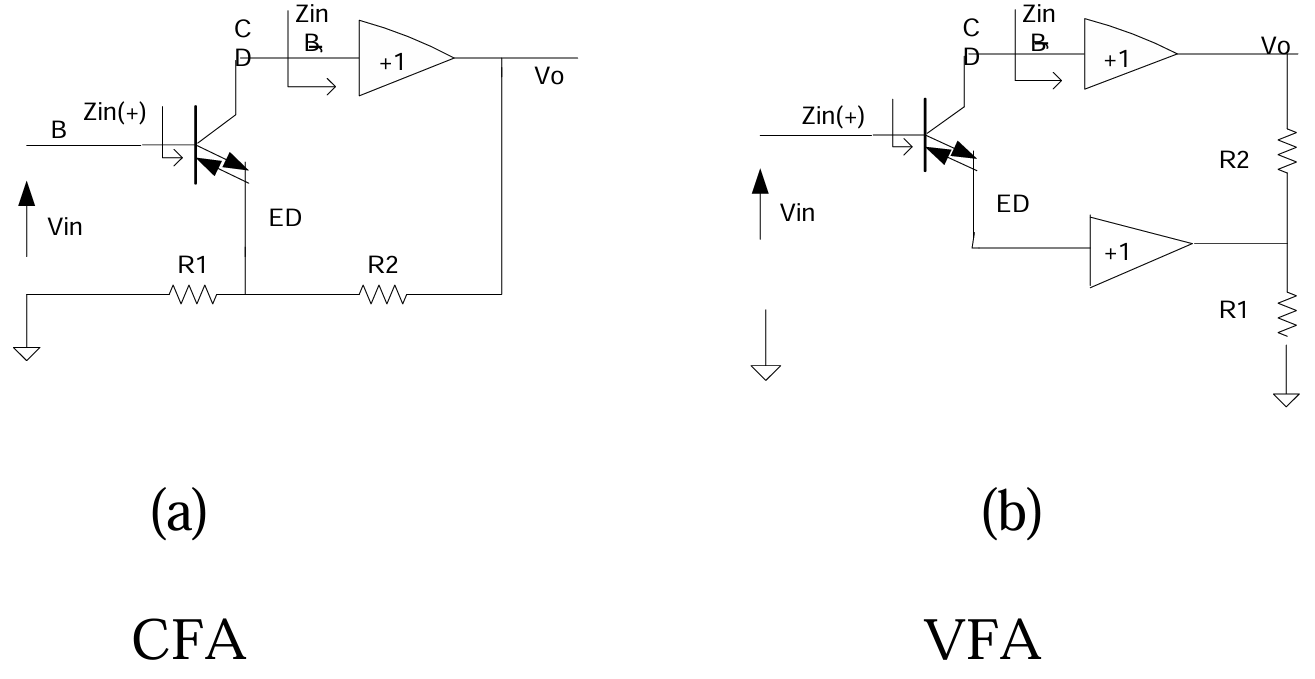
\includegraphics[width=0.75\linewidth]{Imagenes/4.20.png}
    \caption{}
    \label{fig:4.20}
\end{figure}
\newpage
\section{Estabilidad de los amplificadores realimentados}
\subsection*{Introducción}
El concepto de transformación y la consecuente modificación del ancho de banda del sistema básico con función de transferencia de un solo polo, producido por la realimentación negativa se extienden al caso en que aquel tenga una función multipolo.

En efecto, sea la ganancia de lazo abierto, en Fig. \ref{fig:5.1} expresable por (\ref{eq:5.1})
\begin{figure}[H]
    \centering
    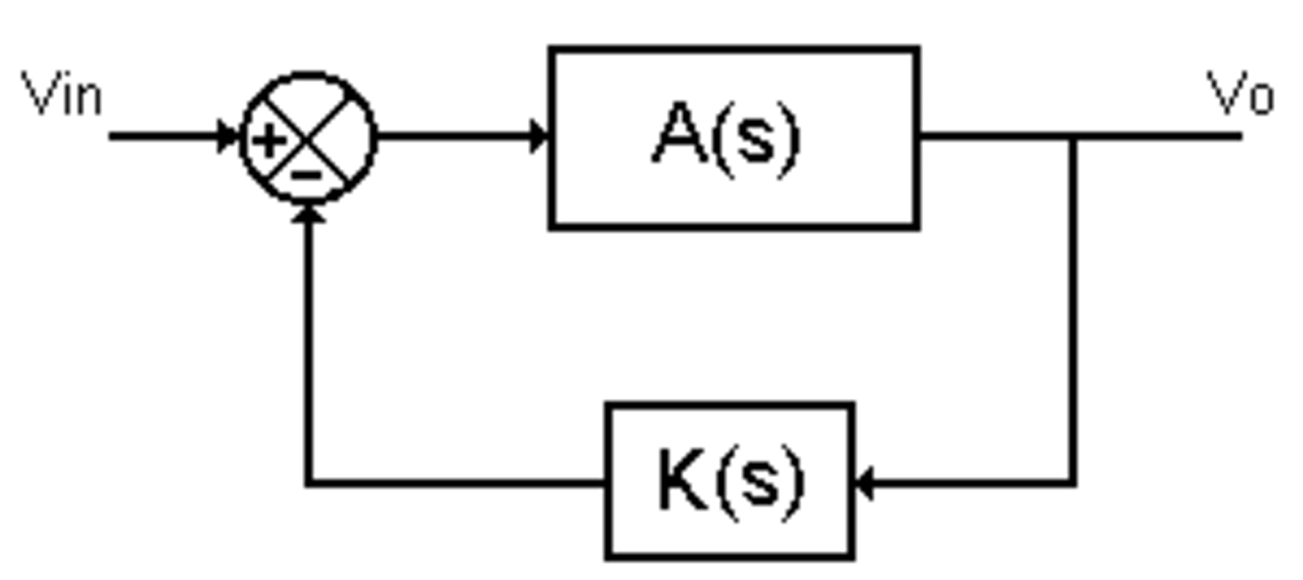
\includegraphics[width=0.5\linewidth]{Imagenes/5.1.png}
    \caption{}
    \label{fig:5.1}
\end{figure}
\begin{equation}
A_v(s) = \frac{A_v(0)}{D(s)}
\tag{5.1}
\end{equation}

En (5.1), el polinomio denominador $D(s)$, es racional a coeficientes reales en la frecuencia compleja. Si este sistema es realimentado negativamente por ejemplo con una red resistiva pura ($K=$ real), la ganancia de lazo cerrado (GLC), es

$$
A_{vf}(s) = \frac{A_v(s)}{1 - T(s)}
$$

Donde la ganancia de lazo (GL),

\begin{equation}
T(s) = -K \cdot A_v(s)
\tag{5.2}
\end{equation}

Luego se deduce para (GLC)

\begin{equation}
A_{vf}(s) = \frac{\frac{A_v(0)}{D(s)}}{1 + K \cdot \frac{A_v(0)}{D(s)}} = \left( \frac{A_v(0)}{D(s) + K \cdot A_v(0)} \right) = \frac{A'_v(0)}{D'(s)}
\tag{5.3}
\end{equation}

En la expresión (5.3), se puede ver que además de modificar la ganancia en continua también lo hace con la distribución y característica de los polos de la función de transferencia original ($A_v(s)$). Si la GLA del sistema básico tiene un solo polo (secc.2.2), la realimentación negativa introducida lo desplaza sobre el semieje real negativo (Fig. 5.2), tal que para el cien por ciento de realimentación ($K=1$), el polo adquiere una posición extrema, igual a la frecuencia de cruce de la GLA ($f_T$).
$$
f_H = K \cdot f_T \rightarrow f_H = f_T
$$
\begin{figure}[H]
    \centering
    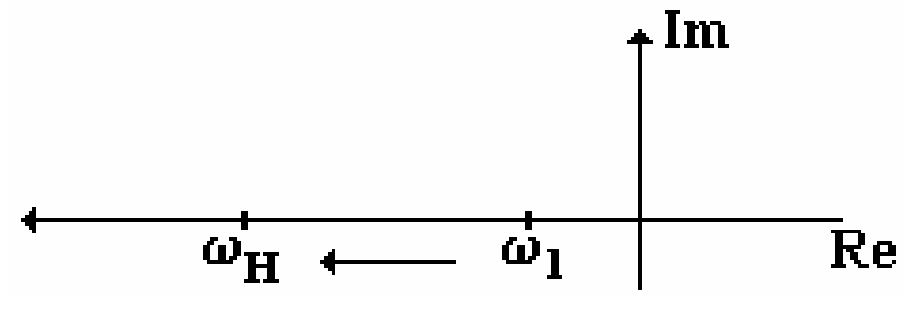
\includegraphics[width=0.5\linewidth]{Imagenes/5.2.png}
    \caption{}
    \label{fig:5.2}
\end{figure}
$\omega_1$ \quad Frecuencia del polo original de GLA. \\
$\omega_H$ \quad Frecuencia del polo de la GLC.

Se verá a continuación que si la ganancia de lazo abierto original, tiene más de un polo la introducción de realimentación negativa suficiente, puede transformar pares de estos en complejos conjugados, generando respuestas que si bien son buscadas en aplicaciones de osciladores y filtros activos, pueden ser inaceptables en amplificadores lineales de banda ancha. Para evaluar cuantitativamente estos efectos es necesario fijar algunos conceptos básicos de estabilidad de sistemas realimentados. Estos se desarrollan a partir de la expresión de la ganancia de lazo cerrado dada por la fórmula de Black, de la que matemáticamente se deduce que si en el lazo hay una señal cuya frecuencia ($\omega_G$) hace cero el denominador, el sistema se hace inestable.

En efecto si:
\begin{equation}
    1 - T(j\omega_G) = 0 \implies A_{vf}(j\omega_G) \to \infty \tag{5.4} \label{eq:5.4}
\end{equation}

La condición anterior implica un crecimiento teóricamente ilimitado de la respuesta ante la excitación de frecuencia apropiada puesta en lazo. La condición (\ref{eq:5.4}) debido a su carácter complejo, implica otras dos

\begin{equation}
    T(j\omega_G) = 1 \implies 
    \begin{cases} 
        |T(\omega_G)| = 1 & \text{(a)} \\
        Arg(T(\omega_G)) = 0 \quad \text{o} \quad 2n\pi & \text{(b)}
    \end{cases} \tag{5.5} \label{eq:5.5}
\end{equation}

Las (\ref{eq:5.5}), dan las ecuaciones de partida para la síntesis de osciladores y para el análisis de la estabilidad de amplificadores de banda ancha realimentados, donde estos últimos se deberán mantener distantes de aquella condición para operación estable. Distancias que indicaran el grado de estabilidad del amplificador y se miden tanto en módulo como en fase, denominándose márgenes. Así el margen de ganancia (MG), indica cuan diferente de uno es el módulo a la frecuencia que satisface la condición de fase (\ref{eq:5.5}b) y viceversa el margen de fase (M$\varphi$), muestra la diferencia de la fase actual y la que satisfaría la condición (\ref{eq:5.5}a) es decir, cuando el módulo de la ganancia de lazo es unitario. \\
Fig \ref{fig:5.3}.
\begin{figure}[H]
    \centering
    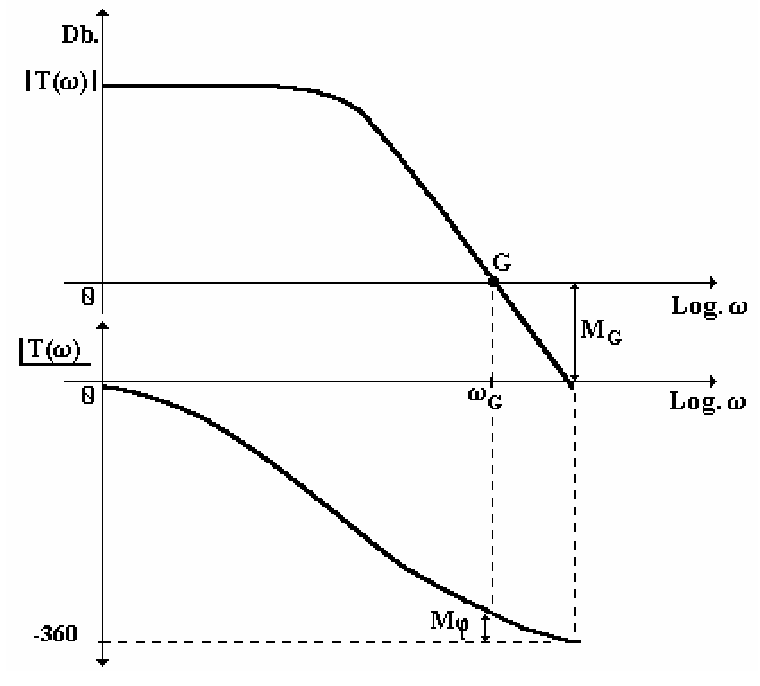
\includegraphics[width=0.5\linewidth]{Imagenes/5.3.png}
    \caption{}
    \label{fig:5.3}
\end{figure}
Existen varios criterios o métodos para evaluar el grado de estabilidad de un sistema ( Nyquist; Mikailov, Bode, etc.). En este texto se utilizaran los diagramas de Bode por su simplicidad.

No obstante cualquiera de los márgenes definidos permiten medir el grado de estabilidad de un sistema, es más utilizado el de fase, debido a que en un amplificador estable la condición de módulo (\ref{eq:5.5}a), se satisface siempre a una frecuencia más baja que la (\ref{eq:5.5}b), tal como lo muestra Fig \ref{fig:5.3}.
Para evaluar cuantitativamente este último y a los efectos de generalizar, se considerará que la red de realimentación es función de la frecuencia ($K(s)$). Luego la ganancia de lazo es según (5.2).

\begin{equation}
    T(s) = -K(s).A_v(s) \tag{5.6} \label{eq:5.6}
\end{equation}

La condición de fase planteada a la frecuencia del punto crítico ($\omega_G$), será teniendo en cuenta que la realimentación negativa introduce un atraso de $180^\circ$, como lo indica la siguiente:

\begin{equation*}
    \angle T(\omega_G) = \angle -1 + \angle K(\omega_G) + \angle A_v(\omega_G) = -180 + \angle K(\omega_G).A_v(\omega_G)
\end{equation*}

\begin{equation}
    M_\Phi = -180^\circ + Arg( K(\omega_G).A_v(\omega_G) ) + 360^\circ = Arg( T(\omega_G) ) + 180^\circ \tag{5.7} \label{eq:5.7}
\end{equation}

En un sistema estable el atraso de fase producido por la ganancia de lazo deberá ser menor de $180^\circ$ y en consecuencia el margen resultará un número positivo.

La frecuencia del punto crítico ($\omega_G$) se evalúa a partir de la condición de módulo

\begin{equation}
    |T(\omega_G)| = 1 \implies \left| A_v(\omega_G) \right| = \left| \frac{1}{K(\omega_G)} \right| \tag{5.8} \label{eq:5.8}
\end{equation}

En este punto es necesario aclarar el sentido que toman los términos involucrados en la expresión de la ganancia de lazo cuando es utilizada en el análisis de estabilidad del amplificador. En primer lugar hay que tener presente que aquella se define como la tendría una señal intercalada en el, cuando la señal que se debe amplificar está pasivada, en este caso particular la señal a insertar en el lazo es el ruido eléctrico siempre presente y cuyo espectro infinito puede aportar la componente que satisfaga las expresiones (\ref{eq:5.5}). El componente de ruido dominante en la mayoría de las aplicaciones es la tensión de ruido interno del amplificador ($v_n$), que por conveniencia es reducido a un modo diferencial equivalente en serie con la entrada  no inversora de aquel (\ref{eq:5.4}), de la misma manera que se hace con la tensión de Offset y RRMC para manifestar su efecto. 
\begin{figure}[H]
    \centering
    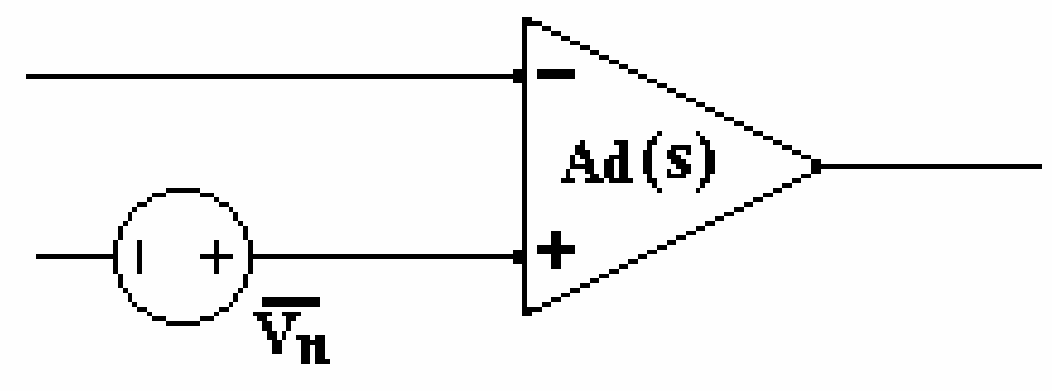
\includegraphics[width=0.5\linewidth]{Imagenes/5.4.png}
    \caption{}
    \label{fig:5.4}
\end{figure}

En base a lo expuesto se puede argumentar que el análisis de estabilidad de una aplicación amplificadora cualquiera, es equivalente a hacerlo con esta excitada por el generador de ruido como muestra la fig \ref{fig:5.4}, luego, la ganancia de lazo de este amplificador resulta, según lo analizado en (1.2), en la siguiente

\begin{equation*}
    T(s) = -K(s).A_d(s)
\end{equation*}

Finalmente, interpretando (\ref{eq:5.8}) en estos términos se obtiene (5.9)

\begin{equation}
    |T(\omega_G)| = 1 \implies |A_d(\omega_G)| = \left| \frac{1}{K(\omega_G)} \right| \tag{5.9} \label{eq:5.9}
\end{equation}

En esta última se distingue que, el primer término se corresponde con la ganancia de lazo abierto del amplificador en configuración no inversora, que además es la que tendría el generador de ruido de fig \ref{fig:5.4}, razón por la cual a la función de transferencia del amplificador básico ($Ad(s)$), se la denomina \textit{ganancia de lazo abierto de ruido}, ( $Ad=GLAn$), mientras que el segundo termino es la ganancia no inversora ideal del mismo amplificador, motivo por el cual se la llama también \textit{ganancia de lazo cerrado de ruido}, ($Avfin = 1/K$). A lo largo de este texto se utilizarán indistintamente la simbología dada por (\ref{eq:5.9}) o sus equivalentes arriba definidas.

A partir de (\ref{eq:5.5}) se deduce que el punto crítico (G) se encuentra en la intersección del diagrama de módulo de la $GLAn$ y $Avfin=1/K(s)$ como muestra las fig \ref{fig:5.5}, en la que se ha supuesto una aplicación que utiliza un A.O con ganancia de modo diferencial de un solo polo y red de realimentación resistiva pura ($K=real$).

\begin{gather*}
    A_d(s) = \frac{A_d(o)}{1 + \frac{s}{\omega_1}} \\
    GLAn = A_v(\omega) = A_d(\omega)
\end{gather*}
\begin{figure}[H]
    \centering
    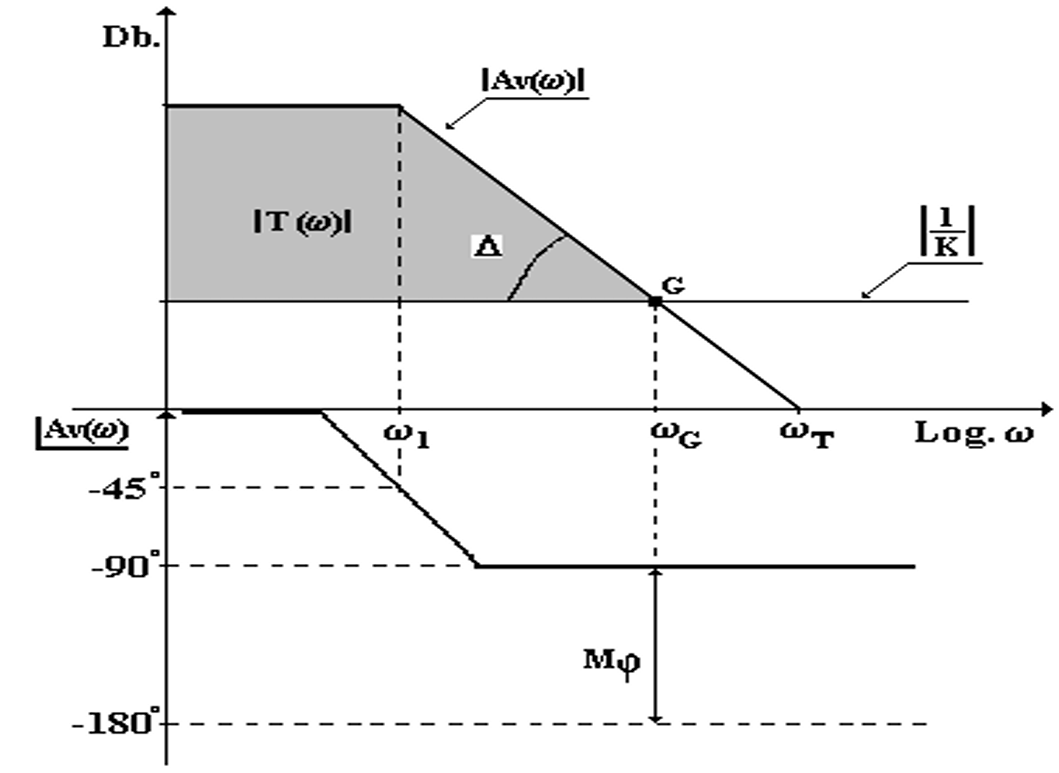
\includegraphics[width=0.5\linewidth]{Imagenes/5.5.png}
    \caption{}
    \label{fig:5.5}
\end{figure}

Del diagrama asintótico se deduce para el margen de fase el siguiente valor

\begin{equation*}
    M_{\Phi} = Arg( T(\omega_G) ) + 180^\circ = Arg( A_v(\omega_G) ) + 180^\circ = 90^\circ
\end{equation*}

Una manera cualitativa de evaluar la estabilidad del sistema es mediante un indicador que es fácilmente identificable en el diagrama de módulos de las magnitudes involucradas y es la pendiente relativa ($\Delta$ )entre la ganancia de lazo abierto y la de ruido ($1/K$) en el punto crítico (G) o de cierre, del diagrama de módulo de T. Si dicha pendiente es menor que - 40 dB/ dec, indicaría cierto grado de estabilidad, tal es el caso planteado en Fig.\ref{fig:5.5} donde $\Delta = - 20 dB/dec$ y el margen de fase igual a $+90^\circ$, mientras que el diagrama de Fig.\ref{fig:5.6}, indicaría inestabilidad, ( $\Delta = -60 dB/dec \Rightarrow M_\phi < 0^\circ$ ).
\begin{figure}[H]
    \centering
    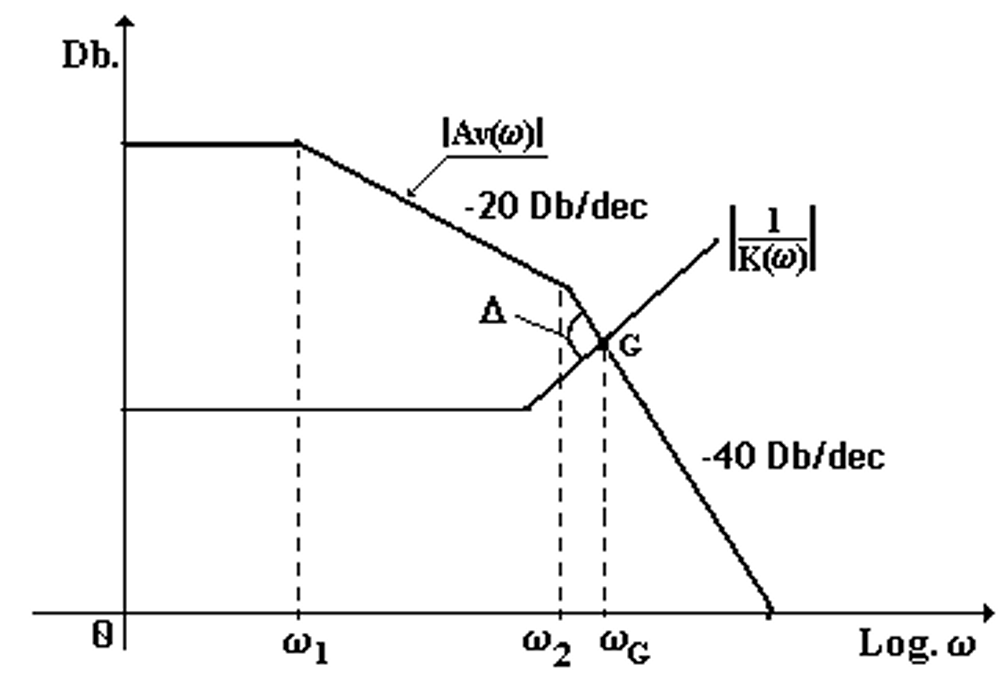
\includegraphics[width=0.5\linewidth]{Imagenes/5.6.png}
    \caption{}
    \label{fig:5.6}
\end{figure}

\subsection{Sistema con Ganancia de Lazo de Dos Polos}
Un sistema con ganancia de lazo de dos polos, puede llegar a tener un comportamiento dinámico inaceptable para operar como amplificador, según sea la cantidad de realimentación introducida.

En efecto si:

\begin{equation}
    T(s) = -K(s).A_d(s) = \frac{-To}{\left(1 + \frac{s}{\omega_1}\right).\left(1 + \frac{s}{\omega_2}\right)} \tag{5.10} \label{eq:5.10}
\end{equation}

El margen de fase será :

\begin{equation}
    M\phi = -\left( \text{tg}^{-1}\left(\frac{\omega_G}{\omega_1}\right) + \text{tg}^{-1}\left(\frac{\omega_G}{\omega_2}\right) \right) + 180^\circ \tag{5.11} \label{eq:5.11}
\end{equation}
\[ \omega_G \to \infty \quad \Rightarrow \quad M\phi \to 0^\circ \]

Se puede analizar el comportamiento dinámico de un amplificador de estas características a partir de la expresión genérica de la GLC dada por (2.12). En efecto normalizando esta en amplitud y relacionándola con T(s) dada por (\ref{eq:5.10}), se obtiene

\begin{gather*}
    A_{vf}(s) = \frac{A_{vfi}}{\left( 1 - \frac{1}{T(s)} \right)} \Rightarrow a_{vf}(s) = \frac{1}{\left( 1 - \frac{1}{T(s)} \right)} \\
    a_{vf}(s) = \frac{1}{\left( 1 + \left( 1 + \frac{s}{\omega_1} \right).\left( 1 + \frac{s}{\omega_2} \right) . \frac{1}{T_0} \right)}
\end{gather*}

\begin{equation}
    avf_{(s)} \cong \frac{1}{\left( 1 + \frac{s}{(T_0)}\left(\frac{1}{\omega_1} + \frac{1}{\omega_2}\right) + \frac{s^2}{(T_0).\omega_1.\omega_2} \right)} \tag{5.12} \label{eq:5.12}
\end{equation}

El denominador de (\ref{eq:5.12}) tiene la forma clásica de respuesta de los sistemas de 2do. orden, cuya expresión compacta parametrizada es

\begin{equation}
    a_{vf}(s) = \frac{1}{1 + \frac{s}{\omega_P.Q_P} + \frac{s^2}{\omega_P^2}} \tag{5.13} \label{eq:5.13}
\end{equation}

$\omega_P =$ frecuencia del polo \\
$Q_P =$ factor de calidad a la frecuencia del polo
Las equivalencias entre los coeficientes es de (\ref{eq:5.12}) y (\ref{eq:5.13}) son

\begin{equation}
    \omega_P = \sqrt{T_0.\omega_1.\omega_2} \quad \text{y} \quad Q_P = \frac{T_0}{\omega_P} \left( \frac{\omega_1.\omega_2}{\omega_1 + \omega_2} \right) \tag{5.14} \label{eq:5.14}
\end{equation}

A los efectos de simplificar el análisis de la respuesta de la ganancia de lazo cerrado conviene normalizar en frecuencia la expresión (\ref{eq:5.13}) respecto de la frecuencia $\omega_P$.

\begin{equation*}
    \frac{s}{\omega_P} = \frac{j\omega}{\omega_P} = J\Omega = S
\end{equation*}

Luego la (\ref{eq:5.13}) queda:

\begin{equation}
    a_{vf}(s) = \frac{1}{1 + \frac{S}{Q_P} + S^2} \tag{5.15} \label{eq:5.15}
\end{equation}

Las caracteristicas de los polos de la expresión (\ref{eq:5.15}) definirán las respectivas de la respuesta de lazo cerrado del sistema, en términos del Qp.

\begin{equation*}
    S_{1}; S_{2} = \frac{1}{2} \left( \frac{-1}{Q_P} \pm \sqrt{\frac{1}{Q_P^2} - 4} \right)
\end{equation*}

En efecto de la anterior, se deduce que $Q_P = 0,5$ da el caso crítico (raíces reales iguales) siendo complejas conjugadas para factores de calidad mayores y reales distintas en caso contrario.

El efecto que tiene la cantidad de realimentación (K), sobre la mutación polar se ve en Fig.\ref{fig:5.7}.

Definiendo la relación, (o distancia en escala logarítmica), de frecuencia entre los polos de la ganancia de lazo (\ref{eq:5.10})

\begin{equation*}
    D_P = \frac{\omega_2}{\omega_1}
\end{equation*}

Se puede expresar (\ref{eq:5.14}) como:

\begin{equation}
    Q_P = \frac{\sqrt{T_0.D_P}}{D_P + 1} \cong \sqrt{\frac{T_0}{D_P}} = \sqrt{\frac{K.A_v(0)}{D_P}} \tag{5.16} \label{eq:5.16}
\end{equation}
La (\ref{eq:5.16}) muestra que definida la respuesta a lazo abierto del sistema, la característica de los polos estará determinada exclusivamente por la cantidad de realimentación introducida, tal que para

\begin{align*}
    Q_P = 0.5 &\implies K_{crit} \implies RRI \\
    Q_P > 0.5 &\implies K > K_{crit} \implies RCC \\
    Q_P < 0.5 &\implies K < K_{crit} \implies RRD
\end{align*}

La figura \ref{fig:5.7a}, muestra lo comentado en el plano complejo y la \ref{fig:5.7b} lo hace en módulo y fase de la ganancia de lazo respectivo
\begin{figure}[H]
    \centering
    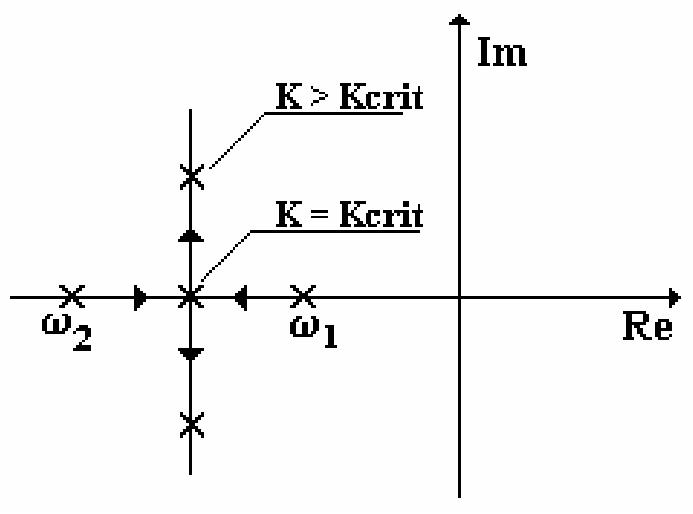
\includegraphics[width=0.5\linewidth]{Imagenes/5.7a.png}
    \caption{}
    \label{fig:5.7a}
\end{figure}

\begin{figure}[H]
    \centering
    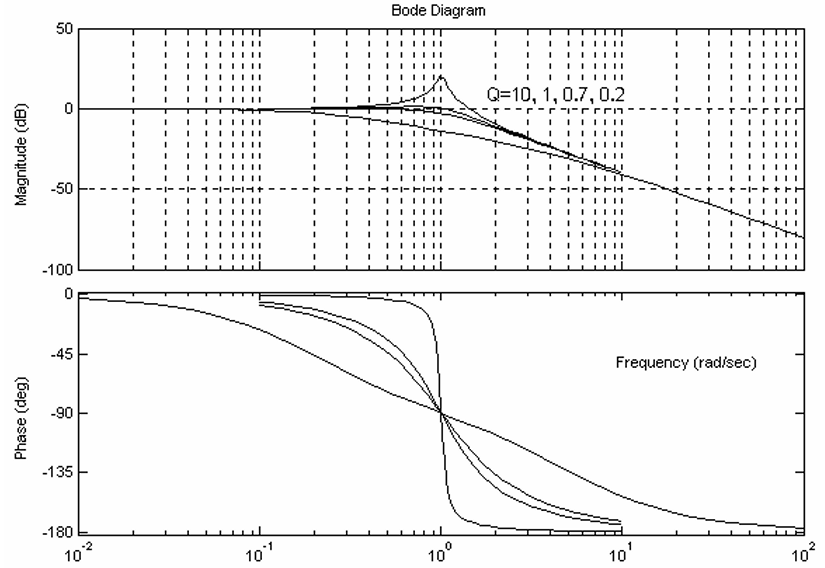
\includegraphics[width=0.5\linewidth]{Imagenes/5.7b.png}
    \caption{}
    \label{fig:5.7b}
\end{figure}
Obviamente el efecto, sobre la respuesta, del tipo de raíces, es sustantivo. Se puede ver que según crece el valor de Qp, la respuesta se aproxima a la producida por un circuito resonante (RLC), casos estos inaceptables en amplificación lineal. Desde este punto de vista aquello debe ser interpretado como un deterioro del grado de estabilidad del sistema. Esto se puede cuantificar midiendo el margen de fase. La fig \ref{fig:5.8} muestra un caso particular en que la frecuencia del punto crítico coincide con el segundo polo de la ganancia de lazo abierto ( $\omega_G = \omega_2$ y $\omega_2 \gg \omega_1$ ). El margen de fase resultante en este caso es

\[
    M\varphi = \left| \underline{K.A_v(\omega_G)} \right. + 180 = - \left( \text{tg}^{-1} \frac{\omega_G}{\omega_1} + \text{tg}^{-1} \frac{\omega_G}{\omega_2} \right) + 180 \cong 45^\circ
\]
En la medida que $\omega_G$ sea mayor que $\omega_2$, disminuye el grado de estabilidad del amplificador.

El factor de calidad (Qp), involucrado se deduce fácilmente teniendo en cuenta el carácter logarítmico del diagrama de módulos de fig 5.8.

\begin{equation*}
    \frac{20 \left( \log A_d(0) - \log \left( \frac{1}{k} \right) \right)}{(\log \omega_2 - \log \omega_1)} = 20 \frac{dB}{dec} \quad \Rightarrow \quad A_d(0).k = \frac{\omega_2}{\omega_1} = D_p
\end{equation*}

Luego de (\ref{eq:5.16}) se deduce Qp=1
\begin{figure}[H]
    \centering
    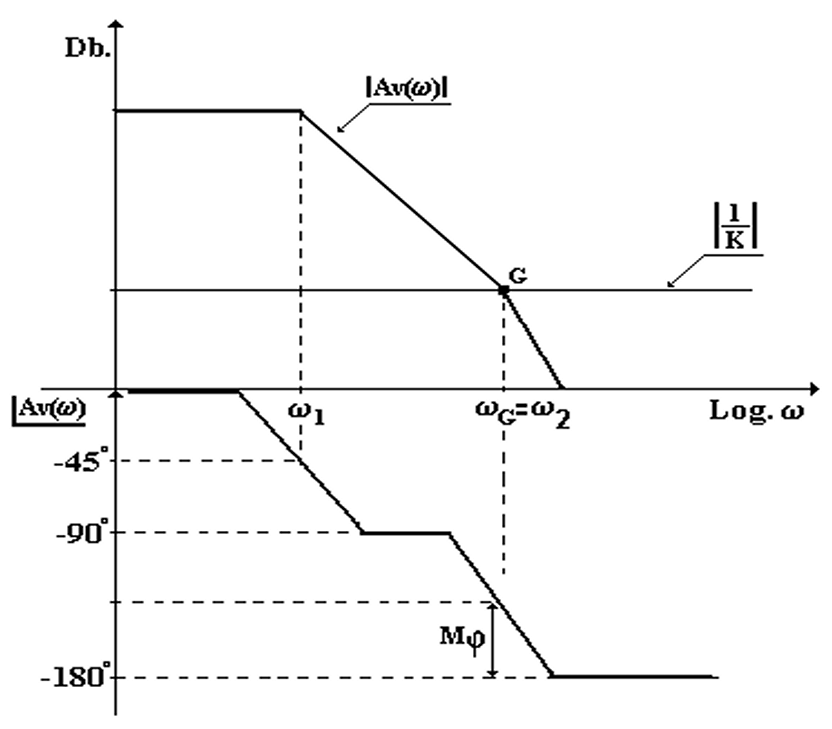
\includegraphics[width=0.5\linewidth]{Imagenes/5.9.png}
    \caption{}
    \label{fig:5.9}
\end{figure}
A la luz del análisis expuesto se entiende el problema de estabilidad que pueden presentar los amplificadores realimentados activamente, aún en el caso que utilicen amplificadores internamente compensados, como es el ejemplo del amplificador logarítmico analizado en la sección 2.2 (E.2.3), cuya estabilidad se analiza en el ejemplo siguiente.
\noindent\rule{\textwidth}{1pt} % Línea 
\textbf{\large Ejemplo 5.1}\\
\noindent\rule{\textwidth}{1pt} % Línea 
\vspace{0.5cm}

Calcular el margen de fase del ampli-log, del ejemplo E 2.3, si el VFA OPA627 utilizado presenta un segundo polo en $f_2 = 50 \text{ MHz}$. \\
El análisis siguiente toma como referencia inicial las figuras y valores de las magnitudes relevantes calculadas en E 2.3.

\vspace{0.2cm}
horizontal
\vspace{0.2cm}

Los datos aplicables del amplificador utilizado son,

\vspace{0.3cm}

OPA 627: \quad $A_d(0)= 116 \text{ dB} \quad f_1= 25 \text{ Hz} \quad f_T= 16 \text{ MHz} \quad f_2= 50 \text{ MHz}$
Teniendo presente que la ganancia de lazo, dependiente de la amplitud de señal resultaba para su valor máximo, ($v_{imax} = 10\text{V} \Rightarrow T_0 = 168 \text{ dB}$ ) y nominando como $A'_d(0)$ a la distancia en dB que hay desde el origen hasta la ordenada correspondiente a la frecuencia $f_2$ , se deduce de la figura E 2.3.2, el margen de fase respectivo.

Teniendo presente el carácter logarítmico del diagrama

$A'_d(0) = f_2 / f_T = 3.13 \implies 9.9 \text{ db} \implies (A_d(0)) = + A'_d(0))_{\text{dB}} \cong 126 \text{ db} = \mathbf{(A)}_{\text{db}}$

$((T_0)_{\text{dB}} - \mathbf{(A)}_{\text{dB}}) / \log(f_G / f_2) = 40 \text{ db/dec} \implies f_G = f_2 \sqrt{(T_0/A)} \cong 561 \text{MHz}$

Con valor de la frecuencia del punto crítico calculada, resulta un margen de fase de $\Phi_M \cong 5^\circ$

Lo reducido de este último resultado se agravaría al punto de llevarlo a oscilación ($\Phi_M = 0^\circ$), si se tienen en cuenta el atraso de fase adicional que producen las capacidades parásitas asociadas a los terminales de entrada del amplificador, (Caso que será tratado posteriormente).
Una manera de mejorar el margen de fase es, disminuyendo la dependencia directa que tiene la ganancia de lazo con señal aplicada, esto es atenuando la cantidad de realimentación $K_0$. Esto se logra por atenuación de la señal a realimentar, con el agregado de una resistencia en serie con el emisor del transistor.
En efecto recalcando la cantidad de realimentación con el agregado de $R_e$ en serie con $h_{ib}$, en el modelo reducido de figura E 2.3.1, se obtiene

\begin{equation*}
    K|_{v_{in}=0} = \frac{V^-}{V'} = g_m . R_1 . \left( \frac{h_{ib}}{h_{ib} + R_e} \right)
\end{equation*}

La anterior muestra la atenuación introducida por $R_e$, que se traslada a la ganancia de lazo.

\begin{equation*}
    T_0 = -I_C . R_1 . \left( \frac{h_{ib}}{h_{ib} + R_e} \right) . \frac{A_d(0)}{V_t} = \left( \frac{V_{in}}{V_t} \right) . \left( \frac{h_{ib}}{h_{ib} + R_e} \right) . A_d(0)
\end{equation*}

La anterior muestra que la resistencia de emisor limitaría el valor de la ganancia de lazo para valores elevados de corriente de colector ($h_{ibmin} = V_t / I_{Cmax}$) y aunque desde este punto de vista convendría que $R_e$ fuera lo más elevado posible, sería a costas de la excursión de la tensión de salida, debido a esto en aplicaciones típicas del amplificador logarítmico, su valor no supera los $5 \text{ k}\Omega$. Asumiendo $R_e = 2 \text{ k}\Omega$, se obtiene para señal de entrada máxima.

$h_{ibmin} = 250 \text{ Ohms}$

$T_0 = 168 \text{ dB} - 20 \text{ dB} = 148 \text{ dB}$

$f_G = f_2 \sqrt{(T_0/A)} = 177 \text{ Mhz} \implies \Phi_M \cong 16^\circ$

Esta mejora relativa del margen de fase es todavía insuficiente para tener una respuesta dinámica aceptable.
Otra manera de analizar la estabilidad del sistema es a través de la respuesta en el dominio temporal, a un escalón de tensión unitaria U(t). Aplicando la transformada inversa de Laplace a la ganancia de lazo cerrado normalizada en amplitud

\begin{equation}
    v_{on}(t) = \mathcal{L}^{-1} [ ( U(s) . a_{vf}(s) ) ] = \mathcal{L}^{-1} \left[ \frac{1}{s} \cdot \frac{1}{D(s)} \right] \tag{5.17} \label{eq:5.17}
\end{equation}

En el caso en que el polinomio denominador tenga raíces reales distintas (caso sobre amortiguado),

\begin{equation*}
    \frac{1}{D(s)} = \frac{1}{(s + a_1)(s + a_2)}
\end{equation*}

La respuesta temporal tendrá únicamente componentes exponenciales decrecientes.

\begin{equation}
    v_{on}(t) = 1 - B \left( \frac{1}{A_1} e^{-a_1 \cdot t} - \frac{1}{A_2} e^{-a_2 \cdot t} \right) \tag{5.18} \label{eq:5.18}
\end{equation}

En cambio si las raíces son complejas conjugadas (caso subamortiguado) aparecen componentes senoidales amortiguadas exponencialmente

\begin{equation}
    v_{on}(t) = 1 - e^{-A \cdot t} ( B_1 \cdot Sen(c \cdot t) + Cos(c \cdot t) ) \tag{5.19} \label{eq:5.19}
\end{equation}

La Fig. 5.9 muestra la respuesta normalizada a un escalón unitario para distintos valores de Qp.

El efecto sensible producido por el aumento de la cantidad de realimentación es el de disminuir el tiempo de crecimiento (tiempo de respuesta) pero a expensas de aumentar la amplitud de los componentes senoidales (rebase o peaking). En la Fig. 5.10 se detallan los parámetros característicos contenidos y definidos a partir de la forma de onda de la respuesta.
\begin{figure}[H]
    \centering
    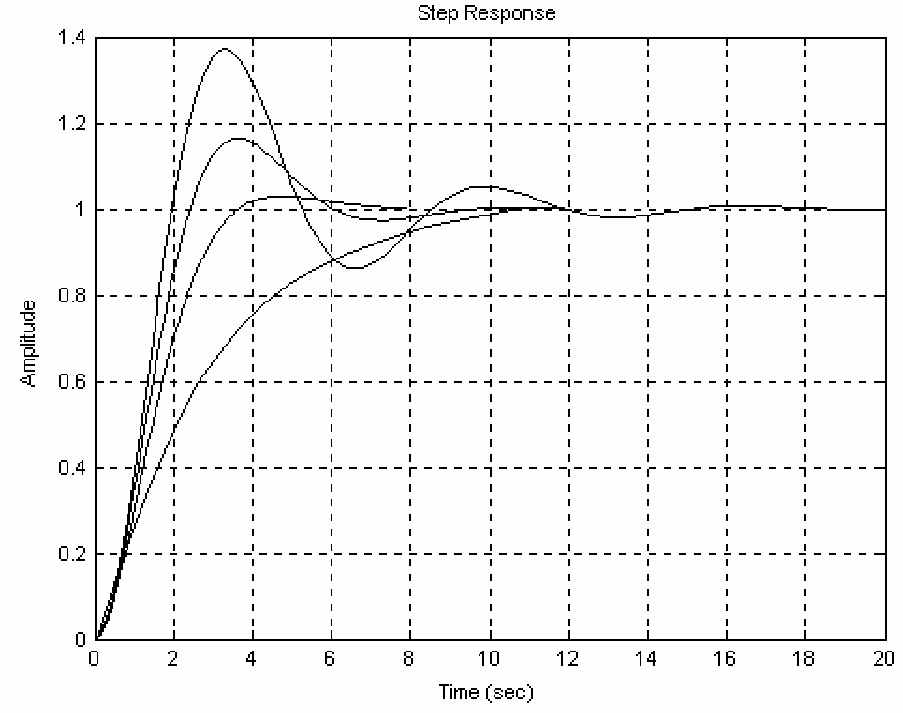
\includegraphics[width=0.5\linewidth]{Imagenes/5.10.png}
    \caption{}
    \label{fig:5.10}
\end{figure}
\begin{figure}[H]
    \centering
    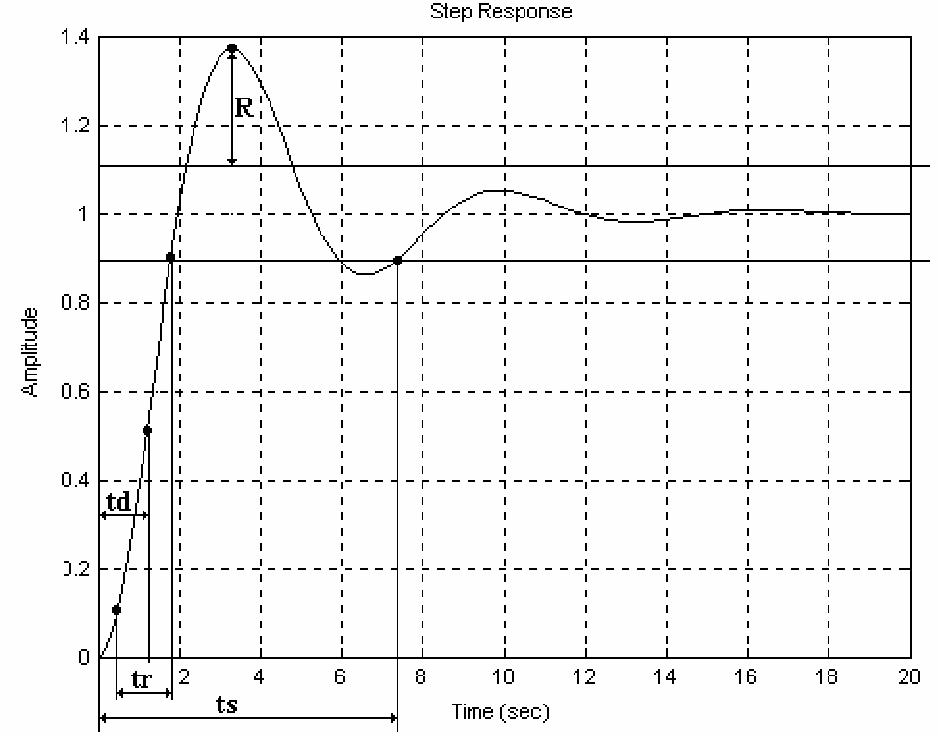
\includegraphics[width=0.5\linewidth]{Imagenes/5.11.png}
    \caption{}
    \label{fig:5.11}
\end{figure}
\begin{itemize}
    \item $t_s =$ tiempo de establecimiento
    \item $t_r =$ tiempo de crecimiento
    \item $t_d =$ tiempo de retardo
    \item $Rebase =$ pico máximo de la respuesta respecto del valor de estado estacionario.
\end{itemize}

En el caso de un amplificador con tres polos reales en lazo abierto se demuestra que, el aumento de la cantidad de realimentación negativa introducida produce reducción del margen de fase que puede hacerse negativo (Inestabilidad).
\subsubsection{Análisis de Estabilidad del CFA}
Si bien los conceptos de estabilidad desarrollados tienen validez general, el caso de los CFA merece un análisis adicional. En efecto el modelo de un solo polo asumido para la transimpedancia dado por (3.1) es suficientemente preciso, para evaluar efectos de primer orden en el comportamiento del dispositivo como lo muestran las expresiones deducidas allí. No obstante, no es difícil intuir que la presencia de componentes capacitivos parásitos asociados a las impedancias de entrada y salida, necesariamente han de agregar otros polos a la transimpedancia y las expresiones con ellas derivadas.

Esto se puede apreciar claramente en los gráficos de magnitud y fase de transimpedancia publicados en la hoja de datos de un dispositivo comercial (OPA 603-BB), mostrado en fig.5.11, en la que se observa un crecimiento abrupto del atraso de fase a frecuencias superiores a los 100 MHz, indicando la presencia de otro polo en las cercanías, en consecuencia debido a que la transimpedancia participa en la expresión de la ganancia de lazo (3.3), es de esperar que en determinadas condiciones de operación se produzca inestabilidad.

Efectuando un análisis cuantitativo del problema a partir de la ganancia de lazo (3.3) expresada a la frecuencia del punto crítico, se obtiene la siguiente relación.

\begin{equation}
    |T(\omega_G)| = 1 = \frac{|Z_T(\omega_G)|}{R_2} \implies R_2 = |Z_T(\omega_G)| \tag{5.20} \label{eq:5.20}
\end{equation}

El margen de fase resulta

\begin{equation}
    \varphi_m = \angle T(\omega_G) + 180^\circ = \angle Z_T(\omega_G) + 180^\circ \tag{5.21} \label{eq:5.21}
\end{equation}


\begin{figure}[H]
    \centering
    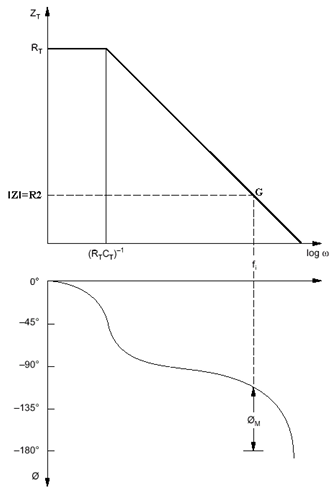
\includegraphics[width=0.5\linewidth]{Imagenes/5.12.png}
    \caption{}
    \label{fig:5.12}
\end{figure}
La expresión (\ref{eq:5.20}) y (\ref{eq:5.21}), permiten definir el método para la selección del valor de $R_2$, a partir de especificación del margen de fase. En efecto fijado este y siguiendo la línea de puntos en los diagramas de Fig 5.11, se determina el valor de la resistencia de realimentación, en el diagrama de módulo de la transimpedancia.

Para operar el dispositivo a frecuencias igual o inferior a la que correspondería un margen de fase de $90^\circ$, se puede considerar válida la expresión de la transimpedancia dada por (3.1) y aplicable el método expuesto para la selección de R2.

\begin{equation*}
    Z_T(s) = \frac{R_T}{1 + s \cdot C_T \cdot R_T}
\end{equation*}
%\printbibliography
\end{document}
